%\documentclass[dvipdfm,final]{pittetd}%   If you want to use dvipdfm. The file is to be normally processed (LaTeX), and 
%                                   then the program dvipdfm applied to it. This will create the PDF file with bookmarks
%                                   and links. It will also try to convert any PS graphics included.
\documentclass[pdflatex, sectionletters, 12pt, final, phd]{pittetd}    % If you want to use PDFLaTeX instead. This will create the PDF file directly.
%                                   Processing time can be longer. No PS graphics conversion will take place 
%                                   automatically.
%
%Other options: ma, ms, for Master's. 
%11pt, 10pt, font size (12pt is default). 
%final, makes pittetd's warnings (about things that might go against the Format Guidelines) 
%into error messages. 
%Option 'sectionletters' numbers the chapters with Roman numerals (I, II, etc.), sections with 
%letters (A, B), subsections with numbers (1, 2), and subsubsections with lowercase letters (a, b). 
%The four levels of the enumerate environment receive the same treatment. Within the
%text, however, cross references (\ref} produce `the whole thing,' something like I.A.1 
%instead of only 1.
%
\overfullrule=0pt % remove the bad box indicators

\usewithpatch{graphicx}%            Better \usewithpatch than \usepackage because it makes pittetd look for any 
%                                   available patch for the package. 
\usepackage{amsmath,amsthm}%        But you can't use \usewithpatch for several packages as in this line. The search for
%                                   patches has to be then forced through:
\patch{amsmatch}
\patch{amsthm}
\usepackage[all]{hypcap} % direct links to figures

\usepackage{notoccite}
\patch{notoccite}

\usepackage{cite}
\patch{cite}

% listings
\usepackage{color}
\usepackage{listings}
%\usepackage{setspace}
\definecolor{Code}{rgb}{0,0,0}
\definecolor{Decorators}{rgb}{0.5,0.5,0.5}
\definecolor{Numbers}{rgb}{0.5,0,0}
\definecolor{MatchingBrackets}{rgb}{0.25,0.5,0.5}
\definecolor{Keywords}{rgb}{0,0,1}
\definecolor{self}{rgb}{0,0,0}
\definecolor{Strings}{rgb}{0,0.63,0}
\definecolor{Comments}{rgb}{0,0.63,1}
\definecolor{Backquotes}{rgb}{0,0,0}
\definecolor{Classname}{rgb}{0,0,0}
\definecolor{FunctionName}{rgb}{0,0,0}
\definecolor{Operators}{rgb}{0,0,0}
\definecolor{Background}{rgb}{0.98,0.98,0.98}
\lstdefinelanguage{Python}{
	numbers=left,
	numberstyle=\footnotesize,
	numbersep=1em,
	xleftmargin=2em,
	framextopmargin=2em,
	framexbottommargin=2em,
	showspaces=false,
	showtabs=false,
	showstringspaces=false,
	frame=l,
	tabsize=4,
	% Basic
%	basicstyle=\ttfamily\small\setstretch{1},
	basicstyle=\ttfamily\small,
	backgroundcolor=\color{Background},
	% Comments
	commentstyle=\color{Comments}\slshape,
	% Strings
	stringstyle=\color{Strings},
	morecomment=[s][\color{Strings}]{"""}{"""},
	morecomment=[s][\color{Strings}]{'''}{'''},
	% keywords
	morekeywords={import,from,class,def,for,while,with,if,is,in,elif,else,not,and,or,print,break,continue,return,True,False,None,access,as,del,except,exec,finally,global,import,lambda,pass,print,raise,try,assert},
	keywordstyle={\color{Keywords}\bfseries},
	% additional keywords
%	morekeywords={[2]@invariant,pylab,numpy,np,scipy,pandas,pd,plt},
	keywordstyle={[2]\color{Decorators}\slshape},
	emph={self},
	emphstyle={\color{self}\slshape},
	%
}
%\linespread{1.3}
%%
%\usepackage{listings}
%\patch{listings}

%
%\patch{pittdiss}                   %If you started writing your thesis with the pittdiss class, this patch makes 
%                                   pittetd interpret pittdiss commands.
%\patch{pitthesis}                  Analogous for the pitthesis class.
\title[Graphene-Complex Oxide Heterostructure]{Graphene-Complex Oxide Heterostructure}% The optional argument is the %                                   version of the title that will appear in Acrobat Reader's Document Info dialog box.
\author{Jianan Li}
\degree{Bachelor of Science, Hong Kong Baptist University, 2011}

\date{April 15th, 2019}%             This date is the date of the thesis defense. Default is \today
\year{2019}                        %pittetd will use the current year unless otherwise indicated. So this command is not
%                                   necessary.
\keywords{Physics, graphene, oxide, nanoscale}% This list appears in the field 'Keywords' of Acrobat Reader's Document Info
%                                   dialog box, and also, optionally, after the abstract.
\subject{Physics}%              This fills in the 'Subject' field in Acrobat Reader's Document Info dialog box.
\school{Kenneth P. Dietrich School of Arts and Sciences}%    The name of the school will be preceeded by 'the' unless otherwise specified, as in:
%\school[certain]{department}
%
\chapterfloats%                    Un-comment this to get figures and tables numbered within chapters.
\begin{document}

\raggedbottom
\setlength{\parskip}{0pt}

\maketitle

%
% For the committee membership page, you have to provide the names and affiliations of the members. The first one will 
% be treated by pittetd as the committee chair (thesis/dissertation advisor).
\committeemember{Jeremy Levy, PhD, Department of Physics and Astronomy, University of Pittsburgh}
%\coadvisor{Second advisor, Dept. Aff.}%         This is used if there are two advisors.
\committeemember{W. Vincent Liu, PhD, Department of Physics and Astronomy, University of Pittsburgh}

\committeemember{Gurudev Dutt, PhD, Department of Physics and Astronomy, University of Pittsburgh}

\committeemember{Adam Leibovich, PhD, Department of Physics and Astronomy, University of Pittsburgh}

\committeemember{Di Xiao, PhD, Department of Physics, Carnegie Mellon University}
% etc., as many as needed. For master's theses, the committee may be omitted, naming only the advisor.
\school{Kenneth P. Dietrich School of Arts and Sciences}

\makecommittee

\copyrightpage                     % Uncomment this to get a copyright page.

\begin{abstract}

Graphene and complex-oxide heterostructures are both 2D systems that have initiated numerous research areas. The two-dimensional electron gas (2DEG) in both systems differs in many ways from traditional semiconductor materials. This research is dedicated to integrating these two versatile systems. Conventionally, the transfer of graphene grown by chemical vapor deposition is assisted by poly(methyl methacrylate) (PMMA).  A new transfer method is developed in this research and can protect the graphene against contaminations. The graphene transferred onto the complex-oxide heterostructure substrates using such method is atomically clean with high mobility. Conductive atomic force microscope (c-AFM) writing technique is applied to graphene-complex-oxide heterostructure to reversibly control the charge-neutrality point (CNP) with nanoscale resolution, utilizing the tunability of the complex-oxide substrate. The local electron density and conductivity of the complex-oxide heterostructure interface can be patterned with the c-AFM tip, and the CNP of the proximal graphene is shifted. With this effect, the mixing of edge state in quantum Hall regime on the edge of graphene p-n junctions can be reversibly controlled. Quantization of resistance is observed as a result of the mixing at low temperature, depending on the directions of currents and magnetic fields. Nanoscale devices such as superlattices can also be produced on various two-dimensional material heterostructure by combining these two techniques.

\end{abstract}
% If you say \begin{abstract}[Keywords:] instead of the simple \begin{abstract}, a list of the keywords is appended.
% The list comes from the \keywords command above.
% The starred version \begin{abstract*} typesets the word `ABSTRACT' on the top of the page
\tableofcontents

\listoftables                      %Pittetd will complain if you tell it to create a list of tables when there are no

%                                   tables (as in this sample file). Uncomment this command if you have tables.
\listoffigures                     %Obvious analogous for figures.
%\preface

% This is the text of the preface, with acknowledgments, dedication, etc. It is optional, and you create, as shown, by 
% just saying \preface and starting the preface's actual text. Note that 'foreword' is no longer acceptable as title
% for this preliminary.
%
%Conventions, such as notation (nomenclature) and abbreviations, don't receive their own preliminary page. They can be included as an appendix, or as part of the introduction.
%
\chapter{Introduction}%
\label{SEC:introduction}

The pursuit for high-performance electronics initiated the study of two-dimensional electron gas (2DEG) systems, where the movements of electrons are free in two dimensions but are confined in the third. Ever since the first generation of 2DEG devices, silicon-based metal-oxide-semiconductor-field-effect transistors (Si-MOSFETs) and III-V-compound-based high-electron-mobility-transistors (HEMTs), were conceived, 2DEG systems have become the fundamental building blocks of modern semiconductor logic circuits for their excellent performances and low energy costs\cite{vinet2017cmos}. The spatial confinement of electrons in the low dimensional systems also allows the emergence of new physics and the advancement of fundamental research. Fabrication technologies such as molecular beam epitaxy (MBE) and modulation doping\cite{dingle1979high} can reduce the electron scattering and makes it possible to produce ultra-high mobility 2DEG devices that lead to the discovery of Quantum Hall effect (QHE)\cite{klitzing1980new} and fractional quantum Hall effect (FQHE)\cite{chang1983fractional}.

Complex oxide heterostructure interface is another class of two-dimensional system. In the seminal work of Ohtomo and Hwang published in 2004\cite{ohtomo2004high}, high-mobility 2DEG is reported to be formed on the interface of LaAlO$_3$/SrTiO$_3$ (LAO/STO). The ``polar catastrophe'' mechanism\cite{nakagawa2006some} of the 2DEG formation on the oxide heterostructure interface resembles the modulation doping in conventional high-mobility semiconductor 2DEG systems that separate dopant from carriers and reduces scattering\cite{bogorin2010laalo3}. Unlike the $s$- or $p$-orbitals in the conventional two dimensional systems such as GaAs/AlGaAs interface, the electrons in LAO/STO are $d$-orbitals\cite{salluzzo2009orbital}, and thus the transport is anisotropic\cite{annadi2013anisotropic}. The interplay of strong electron-electron interactions\cite{hwang2012emergent} and complex band structures from $d$-orbitals\cite{salluzzo2009orbital} gives rise to various physical properties in LAO/STO such as superconductivity\cite{reyren2007superconducting}, magnetism\cite{brinkman2007magnetic}, spin-orbit coupling\cite{caviglia2010tunable}, and electron pairing without superconductivity\cite{cheng2015electron}. The 2DEG is also found to be tunable with external electrical fields\cite{thiel2006tunable} or conductive atomic force microscope (c-AFM) tips\cite{cen2008nanoscale}, and high-quality nanoscale devices can be fabricated on the complex oxide interfaces reversibly\cite{cen2009oxide, irvin2010rewritable, cheng2011sketched, jnawali2015photoconductive, tomczyk2016micrometer, jiang2017direct, chen2019over, sutton2018100, chen2017ultrafast, briggeman2019engineered, hao2019toward, nethwewala2018quantum, tang2017magnetically, pai2019superconductivity, pai2018physics}.

Graphene is the first single-crystal two-dimensional system, and was successfully isolated by the ``scotch tape'' method in 2004\cite{novoselov2004electric} for the first time. The easiness of device fabrication and the rich physics from the unique honeycomb crystal structure of graphene has opened up many new research areas. The electrons near the $K$ and $K'$ points in the reciprocal space can be described by Dirac equations\cite{wallace1947band, neto2009electronic}, and the Dirac-like nature of electrons\cite{novoselov2004electric, zhang2005experimental} leads to exotic properties that rarely observed in other systems. Although the backscattering in graphene is suppressed\cite{ando1998berry}, the mobility is still limited by impurities from device fabrication and substrates in early graphene experiments. In 2010 Dean \textit{et al.} found that hexagonal boron nitride (hBN) serves as perfect encapsulation layers for graphene with minimal charge and phonon scatterings\cite{dean2010naturenano}, and the mobility of graphene can be primarily improved to allow ballistic transport in micron-scale up to room temperature\cite{mayorov2011micrometer}. The mismatch between the hBN substrates and graphene can generate potential superlattice through moir{\'e} patterns. Lattice mismatch in the twisted bi-layer graphene can also modulate the interlayer hybridization and tailor flat-bands with a high density of states, which would enhance strong correlations between electrons and lead to more exotic phases such as Mott insulator\cite{cao2016superlattice, cao2018correlated, chen2018gate} or superconductivity\cite{cao2018unconventional}.

This dissertation is devoted to the integration of graphene and LAO/STO heterostructure, in the hope of discovering new physics from the interaction between these two fascinating 2D systems. Micro-electronics fabrication and c-AFM lithography techniques are utilized for graphene/LAO/STO heterostructure device fabrication. Electronic and optical measurements are performed both in room temperature and 2 K, to probe the electronic and magnetic properties of the graphene/LAO/STO heterostructure devices. Chapter \ref{SEC:introduction} is a general introduction for LAO/STO and graphene. Chapter \ref{SEC:methods} discusses sample growth, device fabrication, and measurement techniques. Chapter \ref{SEC:GCO} is focused on the application of c-AFM writing technique on the graphene devices; two experiments (edge-state mixing and superlattice) are discussed in details to demonstrate the nanoscale control of the graphene charge neutrality point (CNP) using c-AFM. Transport measurement are performed at $T = 2$ K, where LAO/STO is not superconductive and serves as a local gating medium for graphene. Chapter \ref{SEC:Kerr} is devoted to the measurement of the interface magnetism on LAO/STO using magneto-optical Kerr effect. Preliminary data for Kerr imaging of LAO/STO magnetism is presented. Possible experiment improvement using graphene is proposed at the end of the chapter. The last chapter is the conclusion and outlook for future experiments.

\section{LAO/STO heterostructure}

Both LAO and STO have perovskite structures at room temperature. Lattice constant of LAO is $a = 3.791 \ \mathrm{\AA}$\cite{geller1956crystallographic}, while lattice constant of STO is $a = 3.905 \ \mathrm{\AA}$. In each cubic unit cell of STO, the Ti atom is enclosed in an octahedral cage of oxygen, and the octahedron is in the center of a cubic skeleton of Sr atoms (Figure \ref{FIG:STOPhaseTransition}). At $T=105$ K, STO would go through a phase transition, and oxygen octahedron pairs would rotate against each other so that the bonding lengths of Sr--O and Ti--O are optimized\cite{sulpizio2014nanoscale}. This ferroelastic transition would break the cubic symmetry and form tetragonal domains in STO, from different orientations of the tetragonal unit cells. At even lower temperature, the crystal symmetry may transit to orthorhombic and triclinic, but the effects on the property of STO are less significant than the tetragonal phase transition at $T=105$ K.

\begin{figure}[h!]
	\centering
	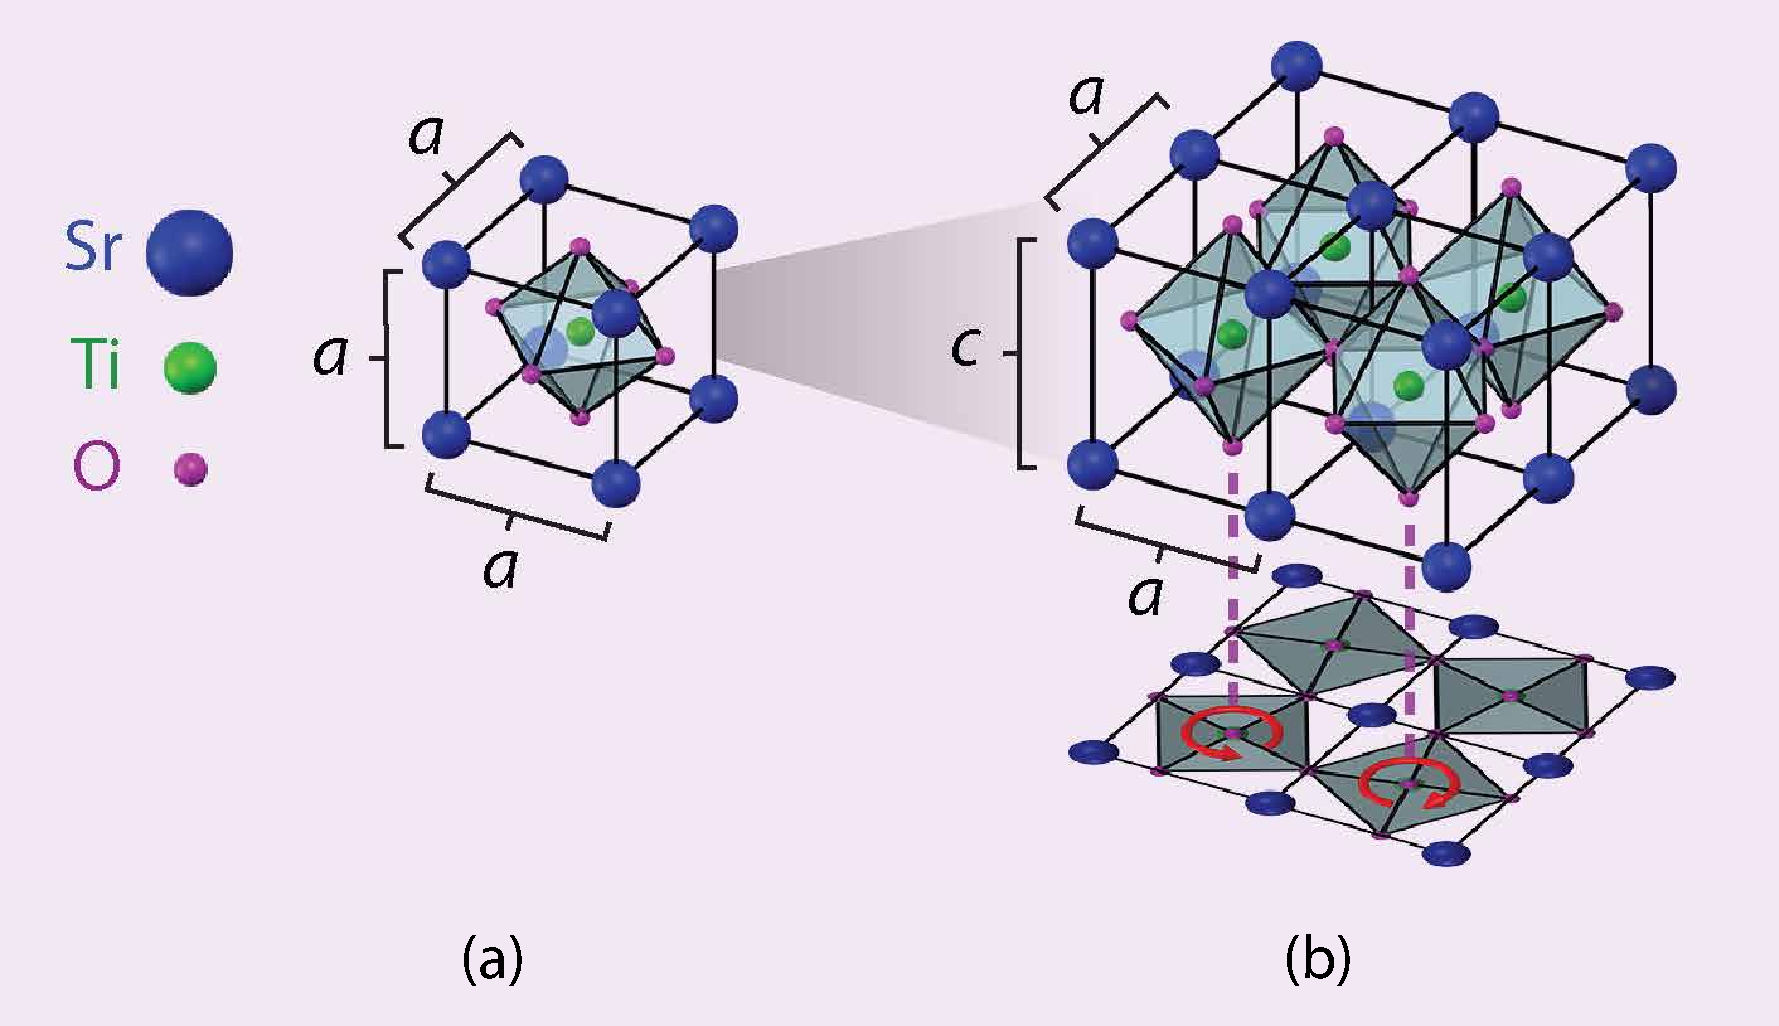
\includegraphics[width=.80\textwidth]{Drawing/STOPhaseTransition.pdf}
	\caption[Ferroelastic transition of STO]{Ferroelastic transition of STO. (a) At $T=300$ K STO has cubic perovskite structure. (b) At $T = 105$ K, the adjacent oxygen octahedrons would rotate in opposite directions and cause ferroelastic transition in STO. Domains will be formed for different orientations of unit cells. Adapted from \cite{sulpizio2014nanoscale}.}
	\label{FIG:STOPhaseTransition}
\end{figure}

At room temperature, the STO is paraelectric, with a large dielectric constant ($\epsilon_r \sim 300$).  When the temperature is lower than $T=105$ K, the paraelectricity persists. Although the elongation of the unit cell in low temperature develops a double-well potential for Ti atoms, with potential minima at the oxygen at opposite sides of the elongation axis, the Ti atoms do not displace towards the minima due to the quantum tunneling of oxygen atoms\cite{sulpizio2014nanoscale} between the minima. STO is one of the few materials that exhibit such \emph{quantum paraelectricity}\cite{muller1979srti}. As a result, the dielectric constant of STO increases rapidly with decreased temperature. The increase is also cut off by quantum tunneling, leaves $\epsilon_r \sim 20,000$\cite{sakudo1971dielectric} at 2 K. This is especially important for gating experiment at low temperature, and more details will be discussed in the following chapters.

The band structure of STO is quite complex. As shown in Figure \ref{FIG:STOBand}, the conduction band is derived from the $3d$ titanium orbitals and the valence band is from the $2p$ oxygen orbitals. The degeneracy of the five $3d$ orbitals is broken by the crystal structure of STO, and then they are grouped into high energy bands $e_g$ (from $d_{3z^2 - r^2}$ and $d_{x^2-y^2}$), and low energy bands $t_{2g}$ (from $d_{xy}$, $d_{yz}$ and $d_{xz}$). Ti $d_{xy}$, $d_{yz}$ and $d_{xz}$ orbitals are coupled to neighboring identical orbitals through the $2p$ orbitals of oxygen atoms in between. Therefore, the hopping matrix elements for in-plane are much greater than for out-of-plane and the transport is anisotropic\cite{sulpizio2014nanoscale}. 

\begin{figure}[h!]
	\centering
	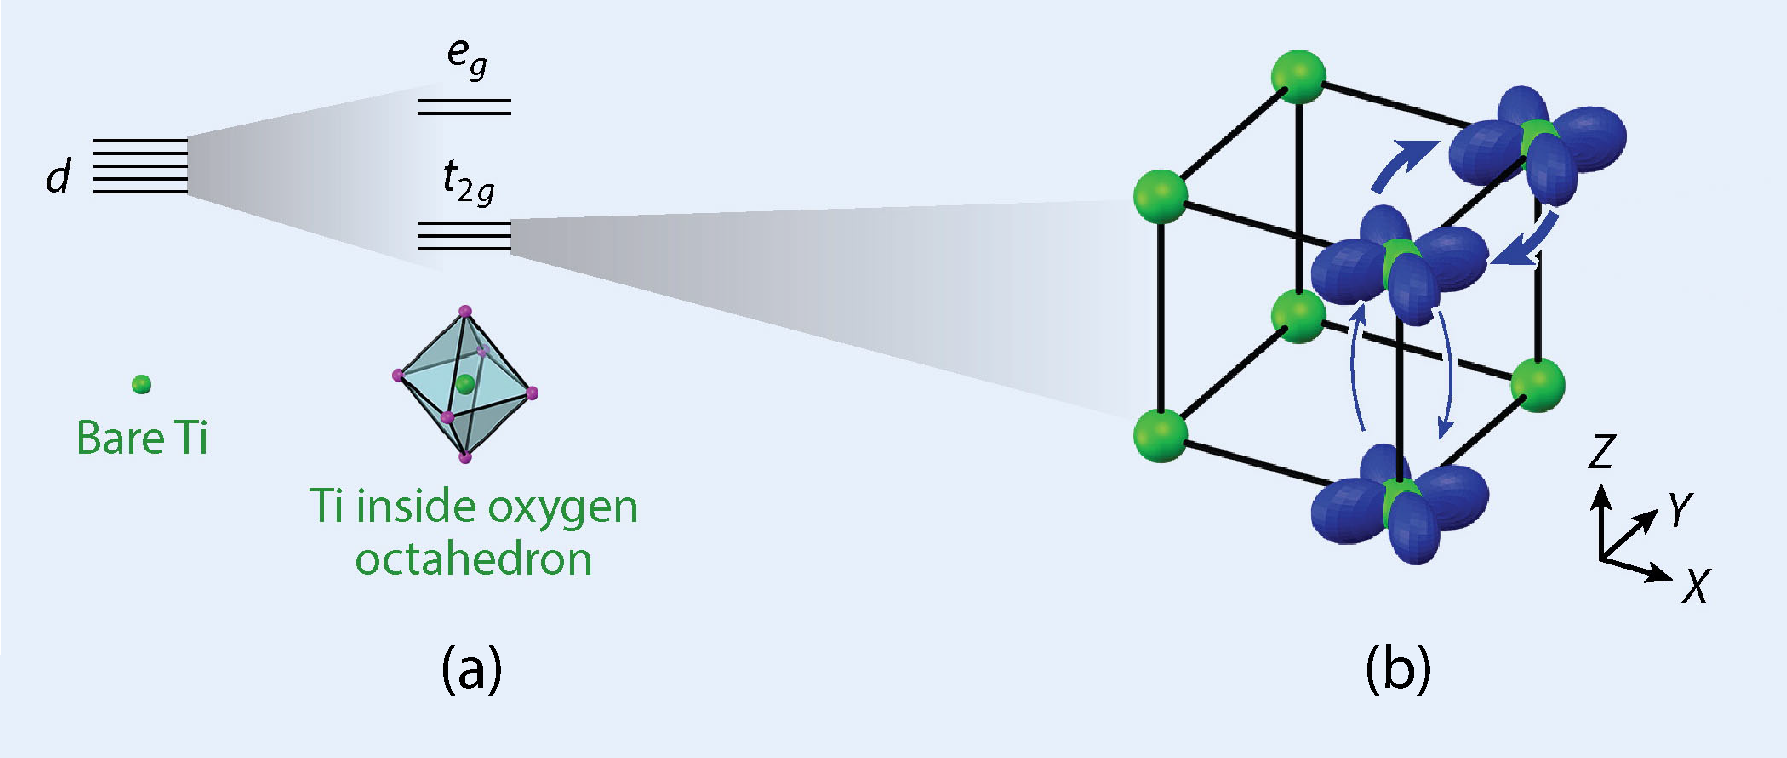
\includegraphics[width=.90\textwidth]{Drawing/STOBand.pdf}
	\caption[The band structure of bulk STO]{The band structure of bulk STO. (a) The conductive bands derive from the $3d$ orbitals of Ti. The degeneracy of the orbitals is broken by the octahedral cage of oxygen atoms, and the energy levels are grouped into $e_g$ and $t_{2g}$. (b) The hopping of $d_{xy}$, $d_{xy}$ and $d_{xy}$ are much easier along in the plane directions, mediated by the $2p$ orbitals of oxygen atoms. Adapted from \cite{sulpizio2014nanoscale}.}
	\label{FIG:STOBand}
\end{figure}

\subsection{2DEG on LAO/STO interface}

Although STO is a band insulator, when LAO is grown epitaxially (the small lattice mismatch of 3\% makes it possible) on TiO$_2$ terminated STO, the interface of LAO and STO becomes conductive, and a layer of 2DEG is formed, first demonstrated by Ohtomo and Hwang in 2004\cite{ohtomo2004high}. The origin of interface 2DEG is still under debate. There are several different theories about the formation of 2DEG on the LAO/STO interface: polar catastrophe\cite{nakagawa2006some}, oxygen vacancy\cite{kalabukhov2007effect} and interfacial cation intermixing\cite{willmott2007structural}. 

The most widely accepted explanation is the polar catastrophe. Unlike the Ti$^{4+}$O$_2^{2-}$ and Sr$^{2+}$O$^{2-}$ planes in STO which are charge neutral, the La$^{3+}$O$^{2-}$ and Al$^{3+}$O$_2^{2-}$ layer are polar, with a net charge of $+e$ and $-e$ respectively. When LAO is grown on TiO$_2$ terminated STO, the polarity will generate a positive electric field, that builds up as the thickness goes up, as shown in Fig \ref{FIG:PolarCatastrophe}(a). To avoid the divergence of potential, the electrons are transferred from the surface to the interface and form 2DEG (Fig \ref{FIG:PolarCatastrophe}(c)). When LAO is grown on SrO terminated STO, a layer of two-dimensional hole gas (2DHG) will be formed in a similar mechanism, as observed by Lee \textit{et al.}\cite{lee2018direct}.

\begin{figure}[h!]
	\centering
	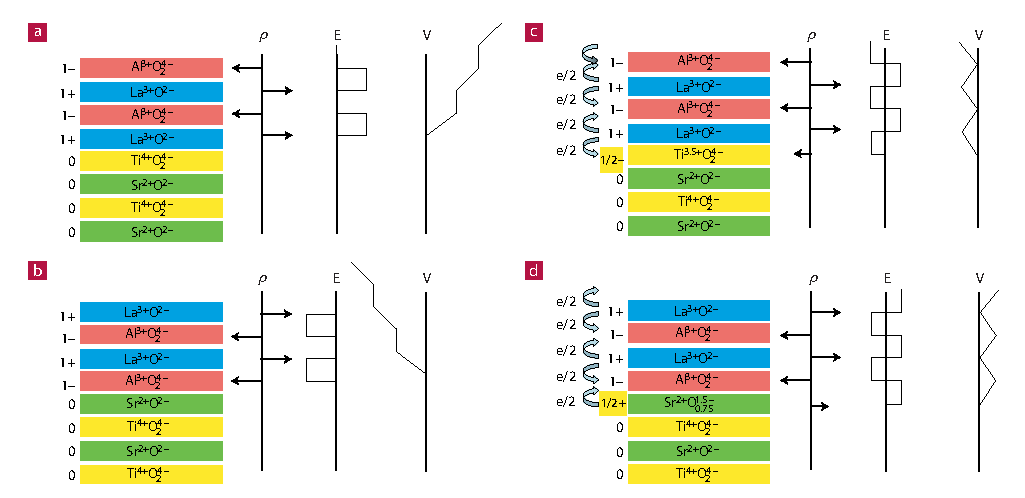
\includegraphics[width=1.0\textwidth]{Drawing/PolarCatastrophe.pdf}
	\caption[Polar catastrophe mechanism of interface conductivity of LAO/STO]{Polar catastrophe mechanism of interface conductivity of LAO/STO. (a) AlO$_2$ and LaO are not charge neutral and a non-zero potential is built up when LAO is grown on TiO$_2$ terminated STO. (c) Electrons are transferred from the top surface to neutralize the potential and therefore a layer of 2DEG is formed. (b) and (d) similar mechanism can explain the formation of hole gas on the interface. Adapted from \cite{nakagawa2006some}.}
	\label{FIG:PolarCatastrophe}
\end{figure}

However, there is a large discrepancy between the carrier density proposed by the polar catastrophe mechanism and measurement. In the polar catastrophe picture, each unit cell will donate half an electron and result in carrier density of $3.2 \times 10^{14}$ cm$^{-2}$, while the observed values are in the order of $10^{13}$ cm$^{-2}$. Also, the formation of 2DEG on amorphous LAO on STO is contradicting to the polar catastrophe model. 

Oxygen vacancy is another possible explanation of the origin of 2DEG\cite{kalabukhov2007effect}; especially it is considered to be the source of the conductivity of bulk STO\cite{schooley1965dependence}. The growth of LAO/STO sample under different oxygen partial pressure also shows that the carrier density is correlated to $P_{\mathrm{O_2}}$, therefore the oxygen vacancies can at least partially explain the formation of 2DEG. The magnetism is also considered related to the oxygen vacancies in STO. There are also TEM\cite{nakagawa2006some}, and XRD\cite{willmott2007structural} evidences support that cation intermixing across the interface can also explain the formation of 2DEG. The exchange of La$^{3+}$ and Sr$^{2+}$ provides extra electrons in the STO. However, this cannot explain the formation of hole gas formation with LAO grown on SrO terminated STO. So far, the polar catastrophe is the most widely accepted explanation of 2DEG in LAO/STO.

Superconductivity has also been found in STO since 1960s'\cite{schooley1964superconductivity}. Interface superconductivity on LAO/STO was first reported by Reyren \textit{et al.} in 2007\cite{reyren2007superconducting}, with a transition temperature $T_c$ of 200 mK. The in-plane and out-of-plane critical fields are around 1 T $\sim$ 2 T and less than 1 T. Recently it was also found that the electron pairing can persist up to a few Tesla, much higher than the critical field of superconductivity, and is possibly induced by a strong correlation between electrons\cite{cheng2015electron, cheng2016tunable}.

LAO and STO are both non-magnetic materials; however, in 2007 the signature of magnetism was discovered on the interface from Kondo-like behavior of interface resistance \cite{brinkman2007magnetic}. More characterization of the interface magnetism were conducted with torque magnetometry\cite{li2011coexistence}, scanning quantum interference device (SQUID)\cite{bert2011direct}, and x-ray circular dichroism (XMCD)\cite{lee2013titanium}. In 2014, Feng \textit{et al.} found that the interface ferromagnetism is electronically tunable at room temperature, from MFM measurement\cite{bi2014room}. Optical measurements of the ferromagnetism will be discussed in Chapter \ref{SEC:Kerr}.

\subsection{Metal-insulator transition and c-AFM lithography}
\label{SEC:WaterCycle}

In 2006, Thiel \textit{et al.} \cite{thiel2006tunable} reported that the interface of LAO/STO shows metal-insulator transition when the LAO is thicker than 4 unit cells (uc). In Figure \ref{FIG:CriticalThickness}(a) when the thickness of LAO is over 4 uc., the interface is conductive. Otherwise, the interface is insulating, and the conductivity is below the measurement limit. When LAO is slightly below the critical thickness (e.g., 3 uc), the conductivity on the interface is tunable, with a voltage applied to the backside of the sample. As Figure \ref{FIG:CriticalThickness}(b) demonstrates, when $V = +100$ V is applied, the interface becomes conductive. When the positive voltage is removed, the resistance is partially restored, but the interface is still conductive. However, when $V = -100$ V is applied, the interface becomes insulating again. 

\begin{figure}[p]
	\centering
	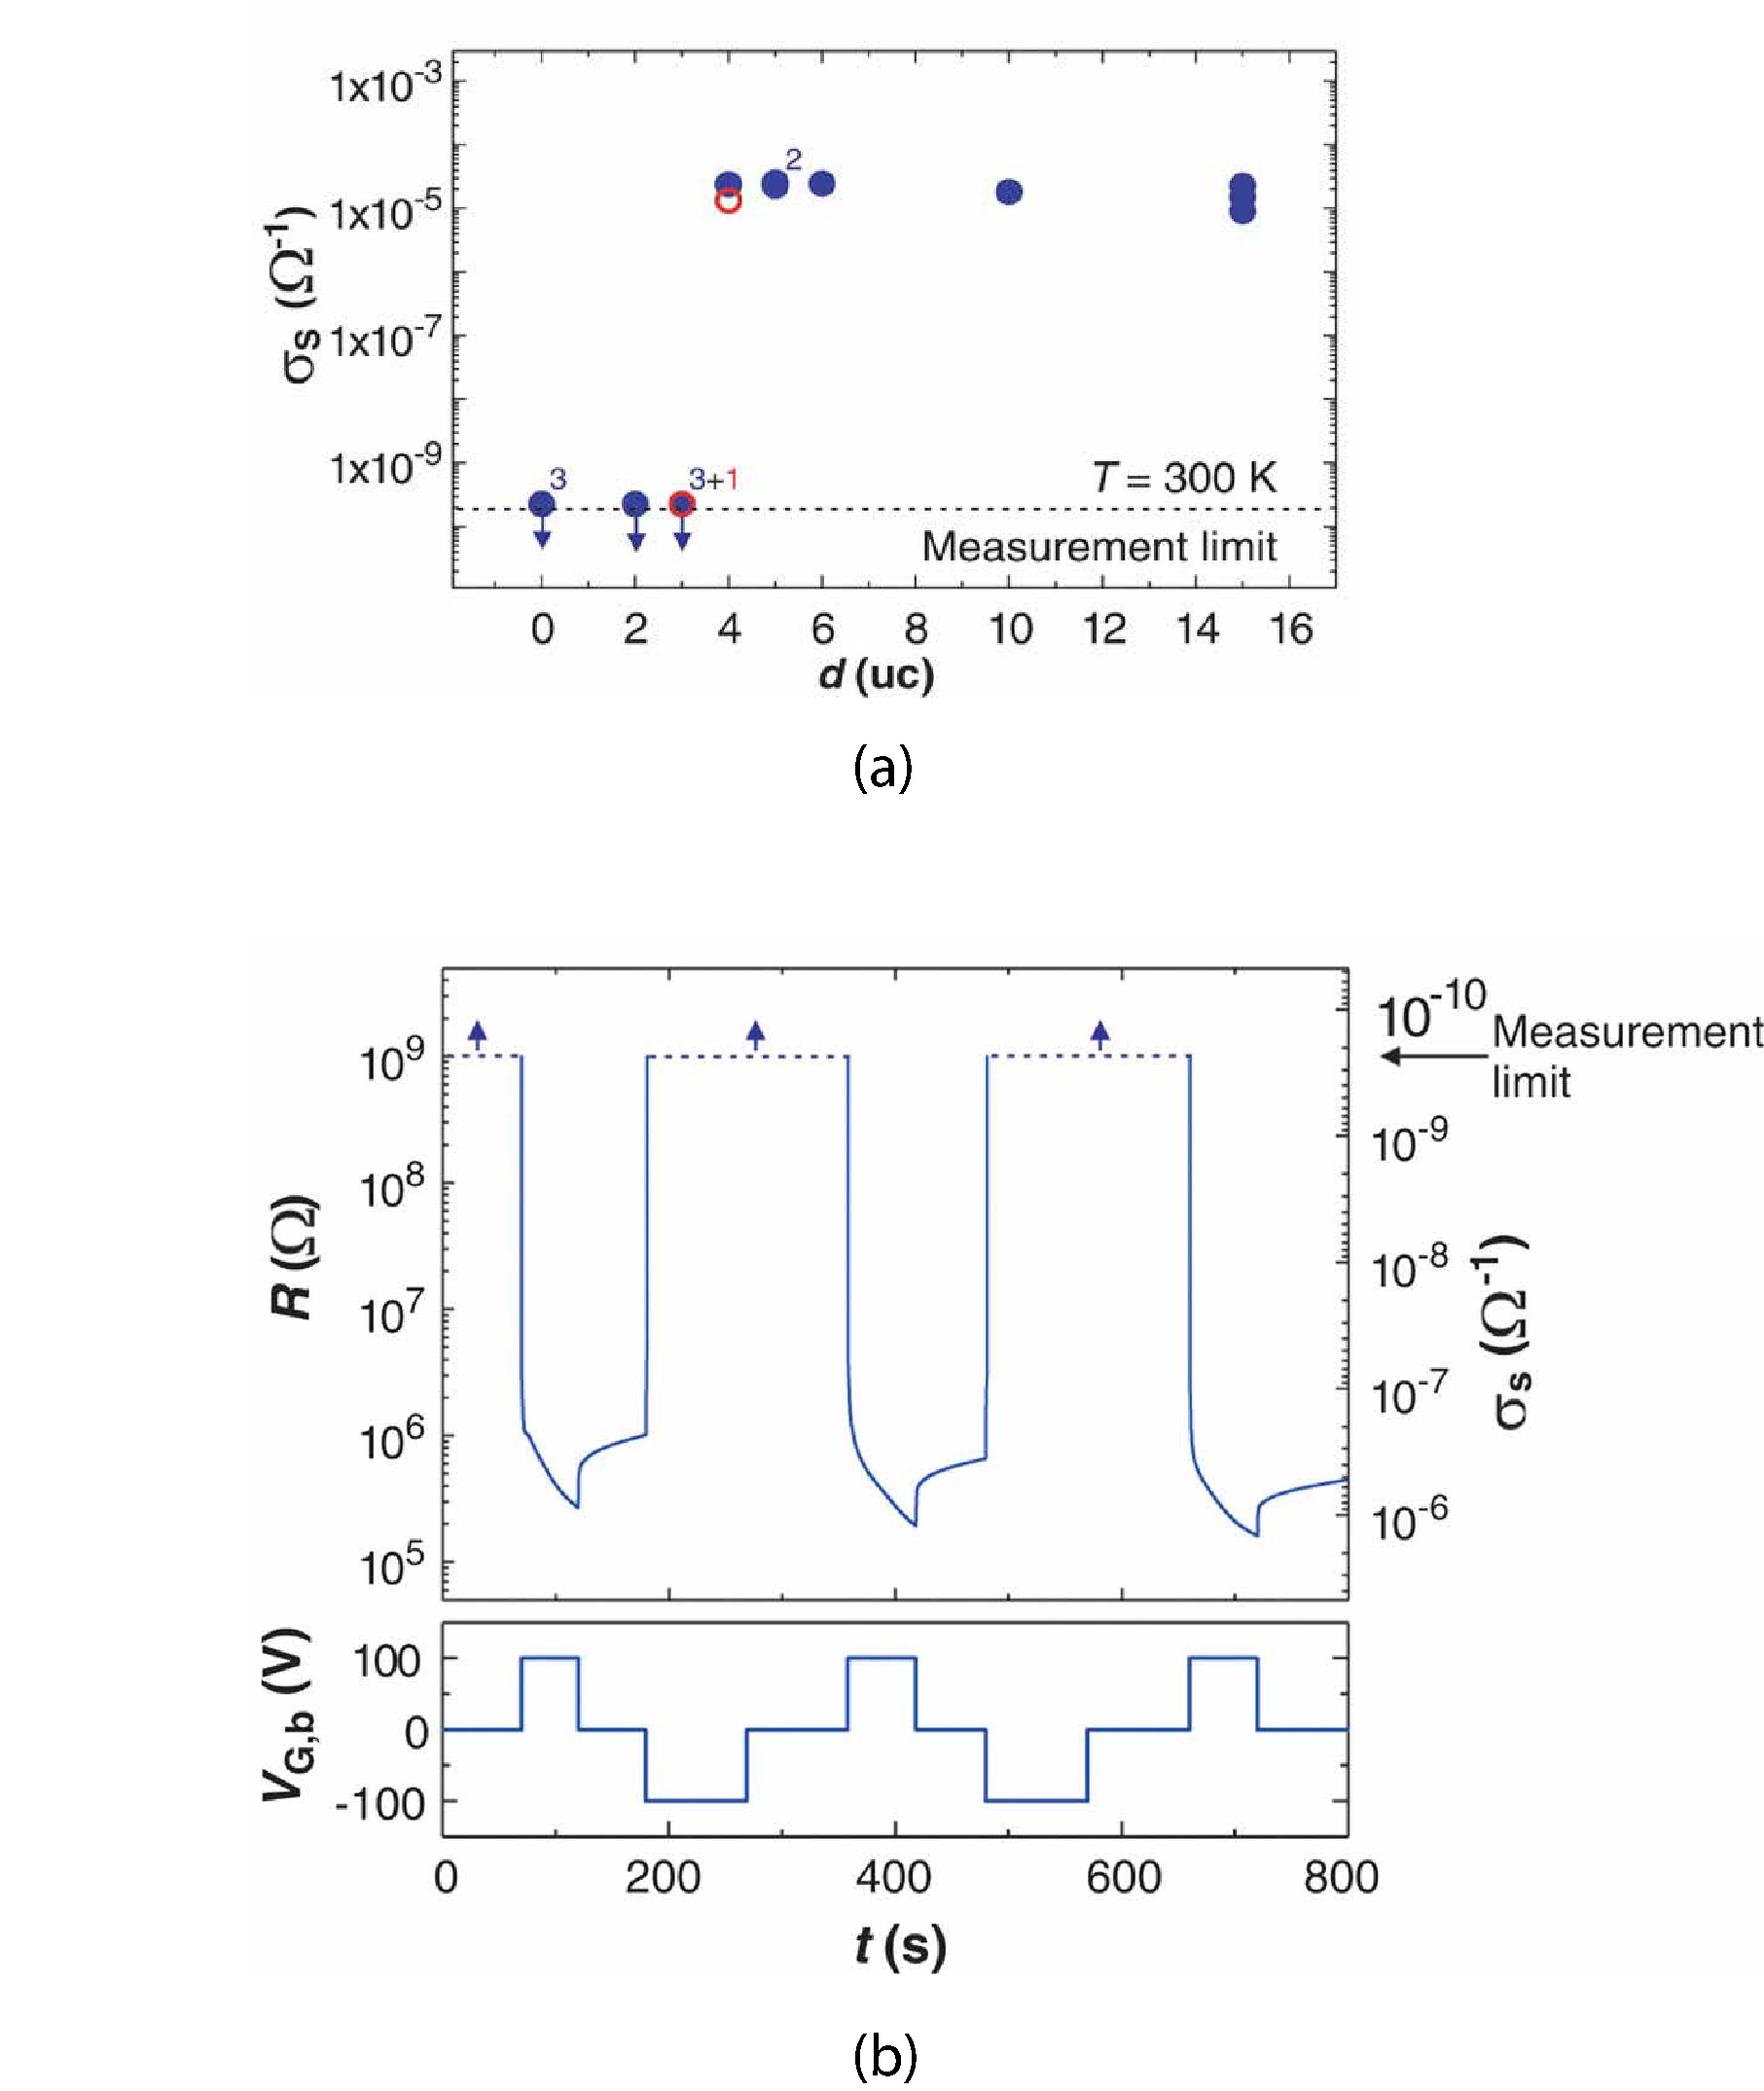
\includegraphics[width=0.8\textwidth]{Drawing/CriticalThickness.pdf}
	\caption[Critical thickness of LAO/STO]{Critical thickness of LAO/STO. (a) When LAO is over the critical thickness of 4 unit cells, the interface is conductive. Otherwise, the interface is insulating. (b) When LAO is only slightly below the critical thickness (e.g., 3 unit cells), the conductivity on the interface is tunable with an external voltage applied to the backside. The as-grown sample is insulating. When $+100$ V is applied, the interface becomes conductive. When the voltage is removed, the conductivity persists. When $-100$ V is applied, the interface becomes insulating again. The conductivity can be cycled with alternating voltages. Adapted from \cite{thiel2006tunable}.}
	\label{FIG:CriticalThickness}
\end{figure}

Following the discovery of backgate tunable interface 2DEG, Cen \textit{et al.}  demonstrated in 2008 that LAO/STO interface conductivity could also be induced with a gate voltage applied with a c-AFM tip on sample surface\cite{cen2008nanoscale}. For a 3 uc LAO/STO sample, the previously discussed polar catastrophe mechanism is not strong enough to reconstruct the band structure and form 2DEG on the interface. With gate voltage locally applied with a nanoscale AFM tip, the positive charge can be transferred on the surface of LAO and build up a potential to cause polar catastrophe. The threshold voltage on the tip is about $V_\mathrm{thresh} \approx 6$ V\cite{cen2008nanoscale}. The width of the conductive channel created in this method is in the same order as the AFM tip, $\sim$ 10 nm. The process is reversible, and the positive charge can be removed with a negative voltage. An insulating gap can, therefore, be created on the nanowire. More experimental details are discussed in Section \ref{SEC:AFMLitho}.

\begin{figure}[h!]
	\centering
	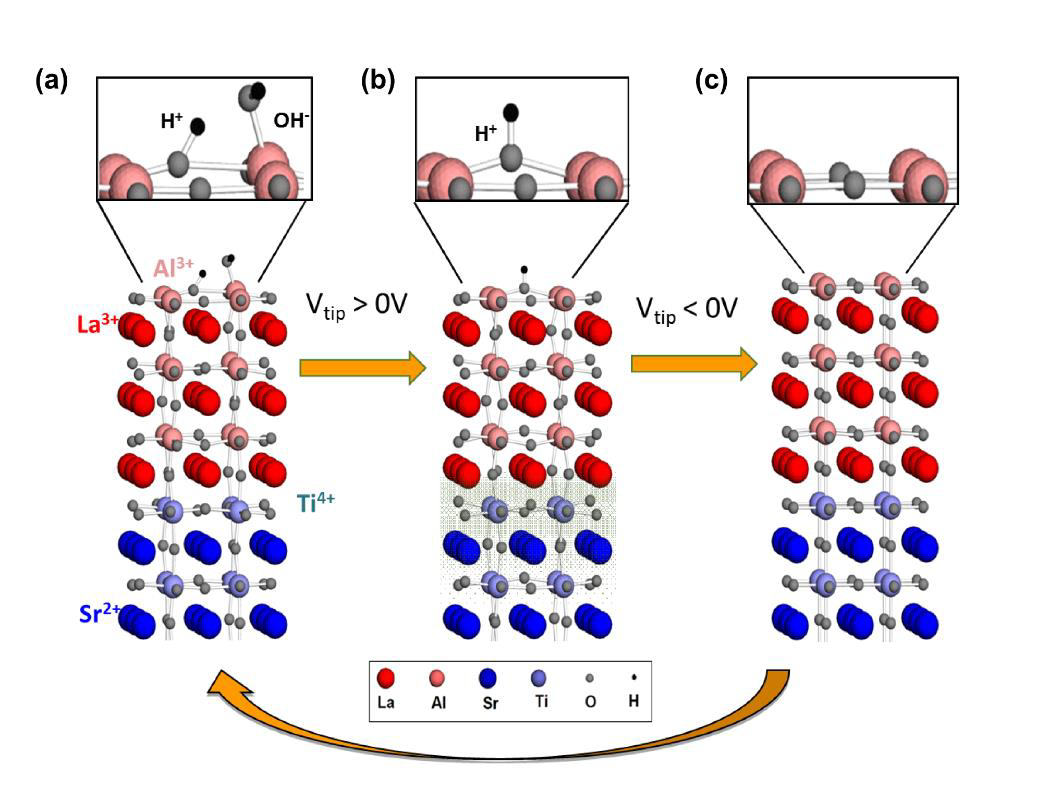
\includegraphics[width=0.9\textwidth]{Drawing/WaterCycle.png}
	\caption[The ``water cycle'' mechanism]{The ``water cycle'' mechanism. A positively biased c-AFM tip removes the OH$^{-}$ and leaves excessive H$^{+}$ on LAO surface, and the positive charges induce 2DEG on the interface underneath. A negatively biased c-AFM removes the H$^{+}$, and restores OH$^{-}$--H$^{+}$ balance. Adapted from Adapted from C. S. Hellberg's APS talk.}
	\label{FIG:WaterCycle}
\end{figure}

The tunability of the LAO/STO with positive c-AFM tip voltage can be explained with the ``water-cycle'' mechanism\cite{bi2010water}. The water adsorbed onto LAO surface is dissociated into OH$^{-}$ and H$^{+}$ (Figure \ref{FIG:WaterCycle}(a)). A positively biased tip removes the OH$^{-}$ and leaves excessive H$^{+}$ on LAO surface, which build up the polar catastrophe potential (Figure \ref{FIG:WaterCycle}(b)). In the erasing process, the negatively biased c-AFM tip removes the H$^{+}$ and restores OH$^{-}$--H$^{+}$ balance, and the interface becomes insulating (Figure \ref{FIG:WaterCycle}(c)). The water cycle mechanism is supported by the control c-AFM writing experiments performed in vacuum\cite{bi2010water}.

\section{Graphene}

Graphene is a single layer of carbon atom ordered in honey-comb structure and was first isolated and studied by Novoselov \textit{et al.}\cite{novoselov2004electric}. It has proved to be a powerful and versatile platform for studying condensed matter phenomena due to the unique crystal structure and Dirac fermion behavior of electrons\cite{wilson2006electrons}. The Dirac cone band structure makes it possible to tune the carrier density continuously between electrons and holes. This duality of carriers in graphene is quintessential foßr many exotic properties, such as Klein tunneling\cite{allain2011klein, katsnelson2006chiral, young2009quantum, shytov2008klein}, edge state mixing\cite{williams2007quantum, abanin2007quantized, lohmann2009four, amet2014selective}, and the ``wedding cake'' structure of quantum Hall states\cite{gutierrez2018interaction}. Band-structure engineering of graphene has been successful using moir{\'e} pattern\cite{dean2013hofstadter, hunt2013massive, ponomarenko2013cloing}, interlayer interaction between twisted graphene\cite{cao2018correlated, cao2018unconventional} and external periodic electric fields\cite{forsythe2018band}. More exotic phases such as Hofstadter butterfly\cite{dean2013hofstadter, hunt2013massive, forsythe2018band}, Mott insulator\cite{cao2018correlated} and superconductivity\cite{cao2018unconventional} have been observed in graphene.

\subsection{Graphene band structure and Dirac fermion}

The band structure was first studied by Wallace \textit{et al.} in 1947\cite{wallace1947band}. The orbital structure of the C atom is $(1s)^2(2s)^2(2p)^4$. The $2s$ and $2p$ orbitals hybridize into $sp^2$ orbitals that form three $\sigma$ bonds with 120$^{\circ}$ angle and a $\pi$ bond that provides free electrons. 

In the honey-comb lattice structure of graphene, there are two inequivalent sublattices that are mirror of each other, which can be labeled with $A$ and $B$. The Bravais lattice is hexagonal, and the primitive lattice vectors can be chosen to be: 
$$\mathbf{a_1} = \frac{a}{2}\left(3, \sqrt{3}\right), \ \ \ \mathbf{a_2} = \frac{a}{2}\left(3, -\sqrt{3}\right)$$
with $a = 1.42 \ \mathrm{\AA}$ being the spacing between to adjacent carbon atoms. Using the relationship between the real space lattice and reciprocal lattice $\mathbf{a_i}\cdot\mathbf{b_j} = 2\pi\delta_{ij}$, the primitive reciprocal lattice vectors can be written as 
$$\mathbf{b_1} = \frac{2\pi}{3a}\left(1, \sqrt{3}\right), \ \ \ \mathbf{b_2} = \frac{2\pi}{3a}\left(1, -\sqrt{3}\right)$$

\begin{figure}[h!]
	\centering
	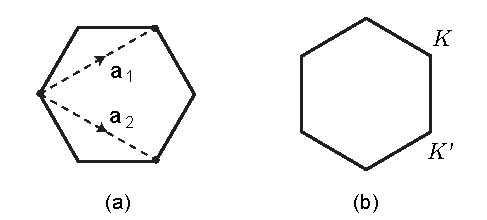
\includegraphics[width=0.6\textwidth]{Drawing/Bravais.pdf}
	\caption[Graphene lattice]{Graphene lattice. (a) Primitive vectors of Bravais lattice. (b) First Brillouin zone of graphene.}
	\label{FIG:Bravais}
\end{figure}

The first Brillouin zone is also in hexagonal shape. There are two types of corners, $K$ and $K'$, and their positions in the reciprocal space are:
$$\mathbf{K} = \frac{2\pi}{3a}\left(1, \frac{1}{\sqrt{3}}\right), \ \ \ \mathbf{K'} =  \frac{2\pi}{3a}\left(1, -\frac{1}{\sqrt{3}}\right).$$

The wavefunction of electron in graphene can be written as the superposition of states in the two sublattices $A$ and $B$:
$$\Psi(\mathbf{k}, \mathbf{r}) = \sum_{\alpha = A, B}c_{\alpha}(\mathbf{k}) \ \Phi_{\alpha}(\mathbf{k}, \mathbf{r}),$$
and the wavefunctions for the sublattice states can be written as Bloch wave functions:
$$\Phi_{\alpha}(\mathbf{k}, \mathbf{r}) = \frac{1}{\sqrt{n}}\sum_\mathbf{R} e^{-i \mathbf{k} \cdot \mathbf{R}} \ \phi_{\alpha}(\mathbf{r} - \mathbf{R}),$$
where $\phi_{\alpha}$ is the wavefunction at each atomic site, R is over the entire Bravais lattice, and $n$ is the number of unit cells in the crystal. 

The tight-binding model assumes that the hopping is only allowed for the nearest and next nearest neighbors, and therefore the Hamiltonian can be written as\cite{wallace1947band, neto2009electronic}:
\begin{equation}
\begin{split}
\mathbf{H} = & - t \sum_{ij=\mathrm{n.n.}, \, \sigma} (a_{i\sigma}^{\dagger} b_{j\sigma} + \mathrm{H. c.}) \\
& - t' \sum_{ij=\mathrm{n.n.n.}, \, \sigma} (a_{i\sigma}^{\dagger} a_{j\sigma} + b_{i\sigma}^{\dagger} b_{j\sigma} + \mathrm{H. c.}),
\end{split}
\label{EQN:Hamiltonian}
\end{equation}
where $t$ is the hopping energy, $a_{i\sigma}^{\dagger}$ is the creation operator for the state on the $i$th site of sublattice $A$ with spin $\sigma\in\{+1, -1\}$, and $b_{j\sigma}$ is the annihilation operator for state on the $j$th site of sublattice $B$ with spin $\sigma$. The summation is over all the nearest neighbors for the 1st term and next nearest neighbors for the 2nd term. For sublattice $A$, the three nearest neighbors in real-space are: 
$$\mathbf{\delta}_1 = \frac{a}{2}\left(1, \sqrt{3}\right), \ \ \ \mathbf{\delta}_2 =  \frac{a}{2}\left(1, -\sqrt{3}\right), \ \ \ \mathbf{\delta}_3 = -a(1, 0),$$
and the next nearest neighbors are:
$$\mathbf{\delta}'_1 = \pm \mathbf{a}_1, \ \ \ \mathbf{\delta}'_2 =  \pm \mathbf{a}_2, \ \ \ \mathbf{\delta}'_3 = \pm (\mathbf{a}_2 - \mathbf{a}_1).$$
The resulting eigen energies are\cite{wallace1947band, neto2009electronic}
$$E_{\pm}(\mathbf{k}) = \pm t \sqrt{3 + f(\mathbf{k})} - t'f(\mathbf{k}),$$
with
$$f(\mathbf{k}) = 2 \, \mathrm{cos}\left( \sqrt{3} k_y a \right) + 4 \, \mathrm{cos}\left(\frac{\sqrt{3}}{2} k_y a \right) \, \mathrm{cos}\left( \frac{3}{2} k_y a \right).$$
The plus sign is for the upper band and minus sign is for the lower band. 

For $\mathbf{k}$ close to $\mathbf{K}$ (or $\mathbf{K'}$), set $\mathbf{q} = \mathbf{K} - \mathbf{k}$, with $|\mathbf{q}| \ll |\mathbf{K}|$, then the band energies can be approximated by a linear dispersion relation
$$E_{\pm}(\mathbf{q}) \approx v_F|\mathbf{q}|,$$
with $\mathbf{q}$ being the momentum $\mathbf{k}$ relative to $\mathbf{K}$ (or $\mathbf{K'}$), and $v_F \approx c/300$ or $10^6$ m/s. The Hamiltonian can be written as 
\begin{equation}
\mathbf{H}(\mathbf{q}) = 
\hbar v_F 
\begin{pmatrix}
0 & q_x + iq_y \\
q_x - iq_y & 0
\end{pmatrix}
=
\hbar v_F \hat{\mathbf{\sigma}} \cdot \mathbf{q}
\label{EQN:DiracHamiltonian}
\end{equation}
in the basis of \emph{sublattice states}, with the components of $\hat{\sigma}$ operator being the usual Pauli matrices. The eigenvectors for states around $\mathbf{K}$ and $\mathbf{K'}$ are
\begin{equation}
\psi_{\pm, \mathbf{K}}(\mathbf{q}) = \frac{1}{\sqrt{2}} 
\begin{pmatrix}
e^{-i\theta_{\mathbf{q}}/2} \\
\pm e^{i\theta_{\mathbf{q}}/2}
\end{pmatrix}, \ \ \
\psi_{\pm, \mathbf{K'}}(\mathbf{q}) = \frac{1}{\sqrt{2}} 
\begin{pmatrix}
e^{i\theta_{\mathbf{q}}/2} \\
\pm e^{-i\theta_{\mathbf{q}}/2}
\end{pmatrix}.
\label{EQN:Eigenstates}
\end{equation}
with 
$$\theta_\mathbf{q} = \mathrm{tan}^{-1}\left(\frac{q_x}{q_y}\right)$$
The plus and minus signs are corresponding to states in the conductance and valence bands. Notice that when $\mathbf{q}$ rotates around $\mathbf{K}$ (or $\mathbf{K'}$), the phase of $\psi_{\pm, \mathbf{K}}$ (or $\psi_{\pm, \mathbf{K'}}$) only changes by $\pi$ instead of $2\pi$ and resembles electron 1/2 spin. Therefore the sublattice states are also called ``pseudo-spin'' states\cite{neto2009electronic}. 

\begin{figure}[h!]
	\centering
	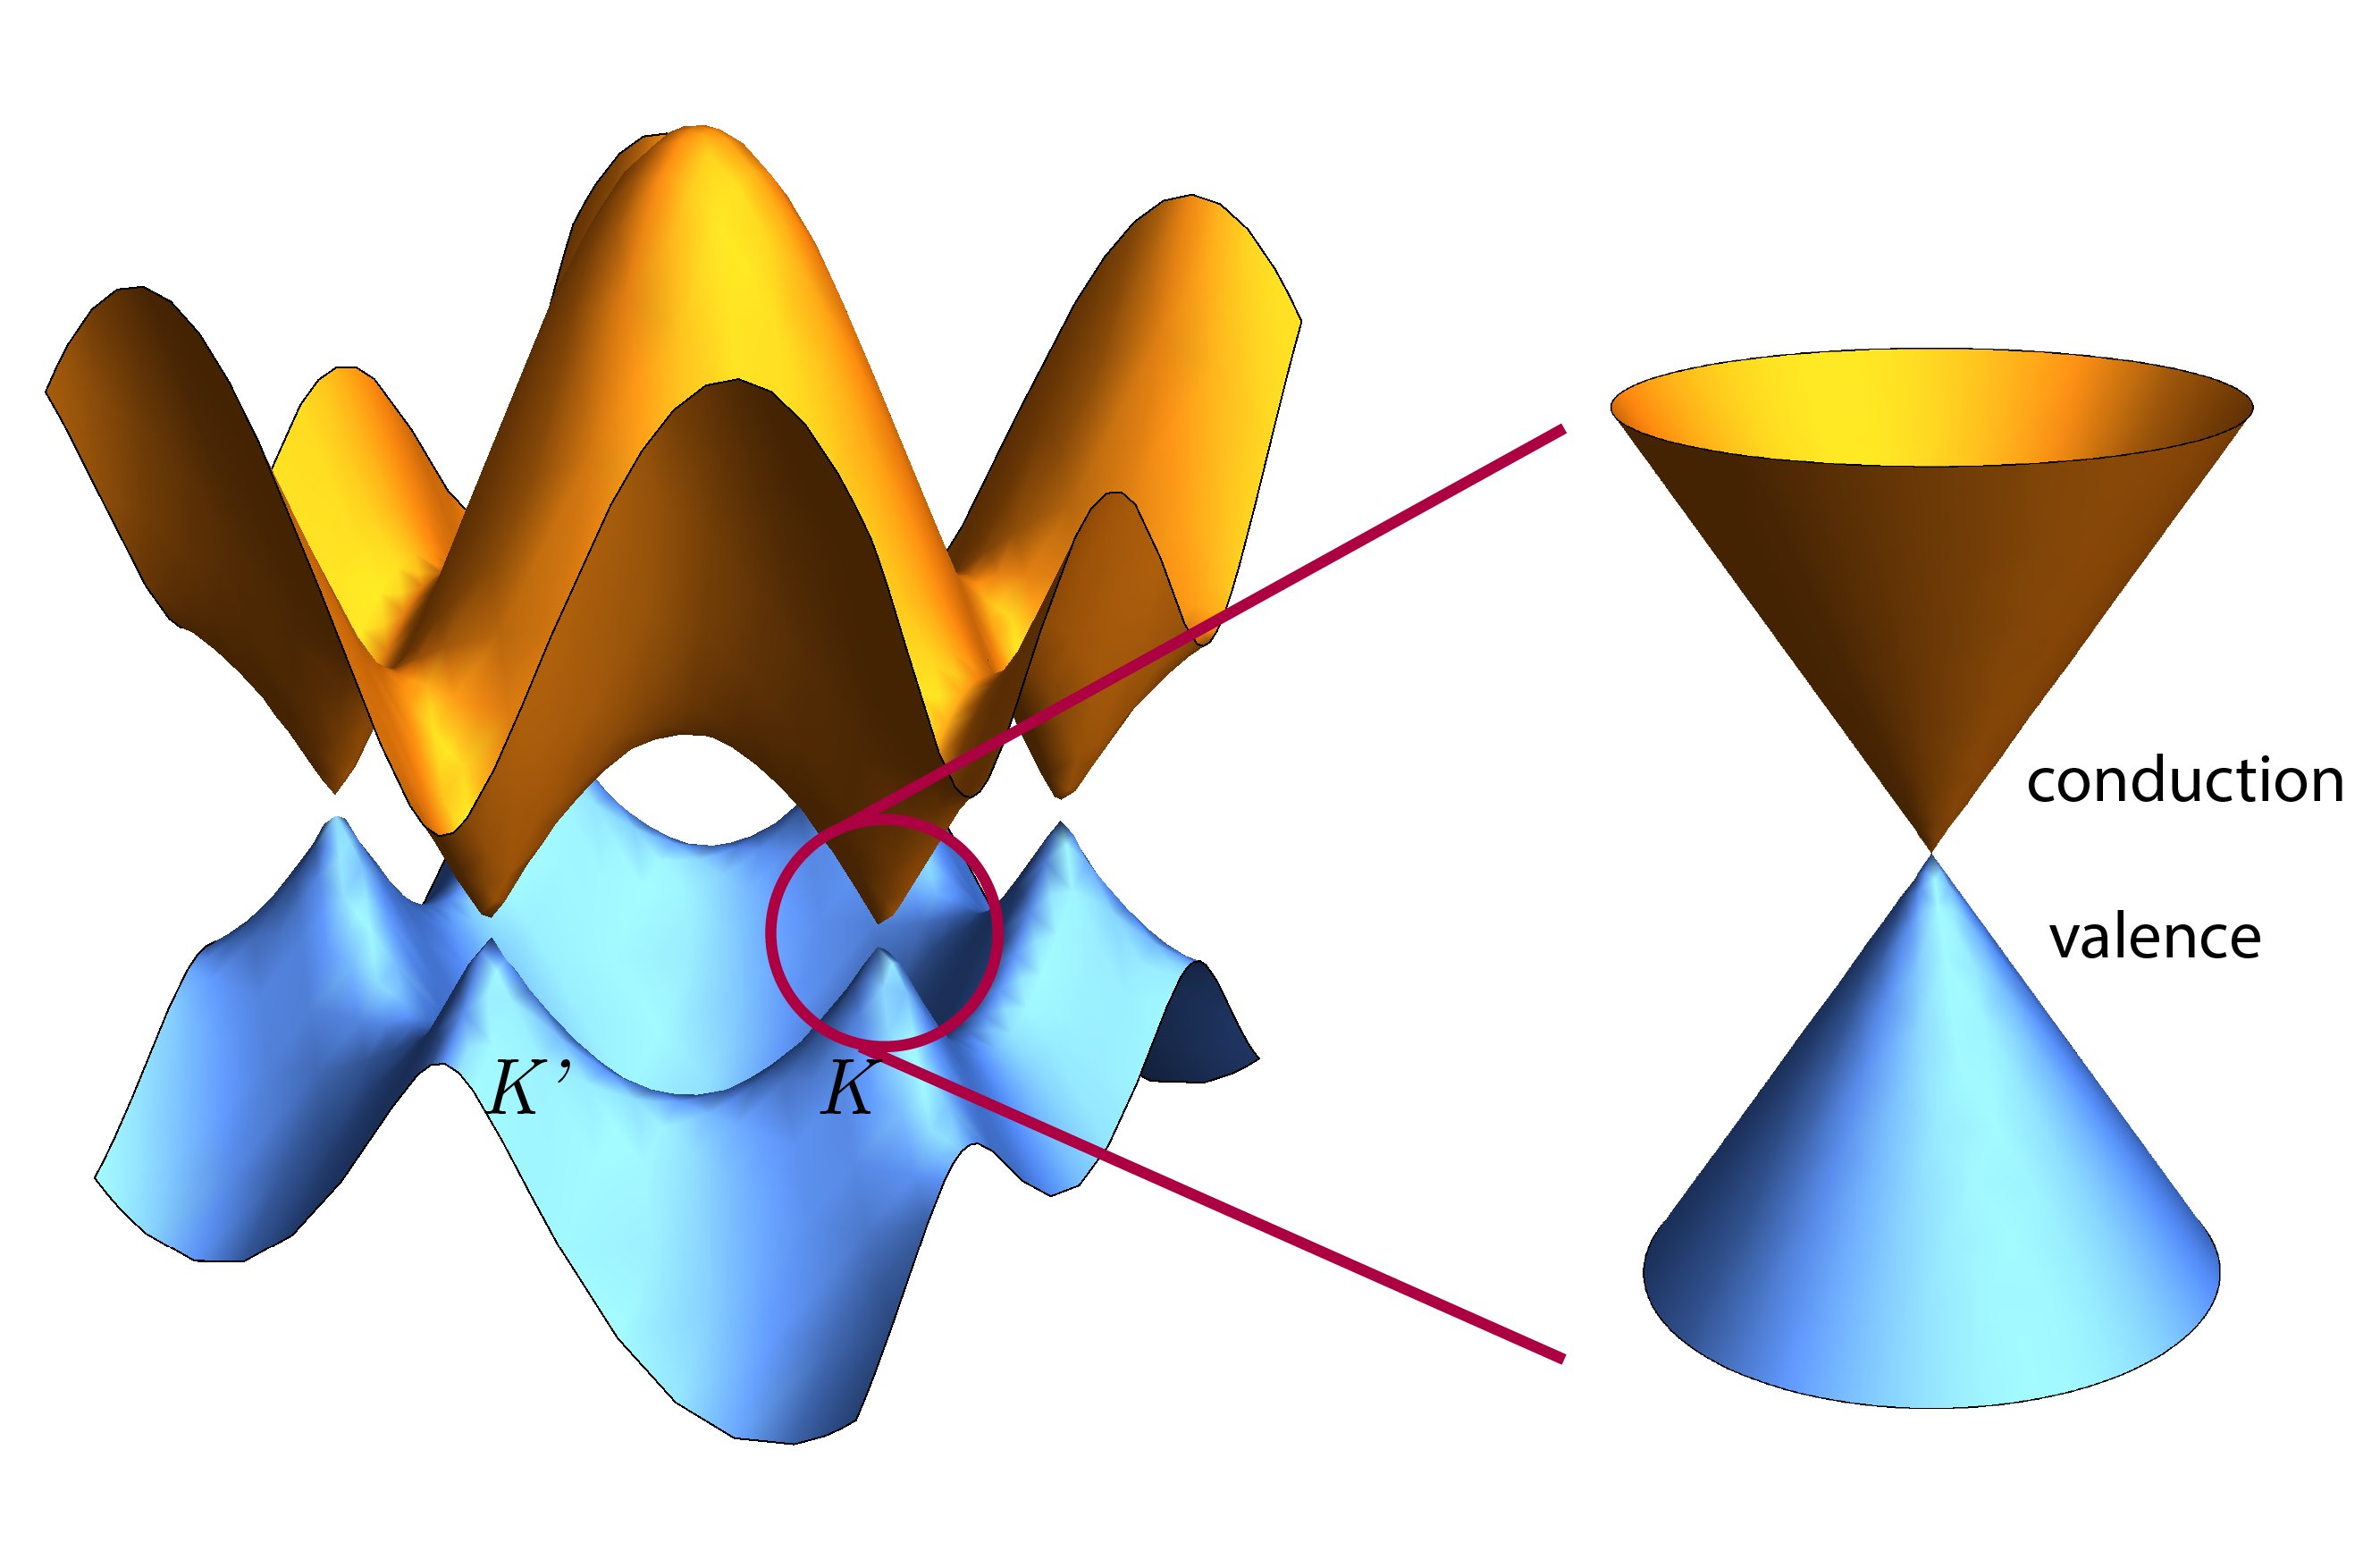
\includegraphics[width=0.8\textwidth]{Drawing/GrapheneBandStructure_zoomin.png}
	\caption[The band structure of Graphene]{The band structure of Graphene. The low energy approximation around $\mathbf{K}$ and $\mathbf{K'}$ has linear dispersion relation. The conduction and valence bands are gapless and the electron behave like Dirac fermions.}
	\label{FIG:GrapheneBand}
\end{figure}

A significant difference between graphene and a conventional semiconductor is that the same wavefunction describes the electron and hole states, and both are obtained from a Hamiltonian of the form of a relativistic particle described by the 2D Dirac equation\cite{neto2009electronic}. Therefore the electrons in graphene have the properties of Dirac fermions, such as handedness. Also notice that the spinors for $\mathbf{q}$ around $\mathbf{K}$ and $\mathbf{K'}$ differ by a phase of $\pi$ (equation \ref{EQN:Eigenstates}). Therefore the states are opposite in handedness around $\mathbf{K}$ and $\mathbf{K'}$. However, at $\mathbf{K}$ and $\mathbf{K'}$ the wavefunctions are still the linear combination of the two sublattice states or the pseudo-spin states. This degree of freedom will introduce extra degeneracies and will be discussed in the following section.

\subsection{Hall effect}

In the classical Hall effect, a Hall voltage will be built by in the transverse direction of current in the magnetic field. In the quantum Hall effect, however, the Hall voltage built up by the magnetic field is quantized. This section will start from the classical behavior of the electron in the magnetic field, and discuss the unique quantum Hall effect in graphene.

\subsubsection{Classical Hall effect}

In the classical Drude model, the electrons are colliding with scattering centers and the average velocity is zero without external electric field. When a field is applied, the drift velocity is 
\begin{equation}
\mathbf{v}_d = -\frac{e\mathbf{E}}{m}\tau,
\label{EQN:ClassicalE}
\end{equation}
where $\mathbf{E}$ is the external field, and $\tau$ is the mean free time between two collisions. The current density can be written as 
$$\mathbf{j} = -ne\mathbf{v}_d = \frac{ne^2\tau}{m}\mathbf{E},$$
where $n$ is the carrier density in the conductor. The conductivity is 
\begin{equation}
\sigma = \frac{\mathbf{j}}{\mathbf{E}} = \frac{ne^2\tau}{m} = n\mu e
\label{EQN:Conductivity}
\end{equation}
and $\displaystyle \mu \equiv \frac{e\tau}{m}$ is the mobility of carrier, which defines how fast the carriers move through a conductor. Usually when the scattering is less likely to happen, the mobility will be higher.

When a magnetic field is applied, the motion equation \ref{EQN:ClassicalE} is modified as 
\begin{equation}
\frac{m\mathbf{v}}{\tau} = -e(\mathbf{E} + \mathbf{v} \times \mathbf{B}).
\label{EQN:ClassicalEB}
\end{equation}
Assume the motion is in $x$-$y$ plane. The Ohm's law can be written as tensor form:
$$
\mathbf{j} = 
\mathbf{\sigma} \cdot \mathbf{E} =
\begin{pmatrix}
\sigma_{xx} & \sigma_{xy} \\
\sigma_{yx} & \sigma_{yy}
\end{pmatrix}
\begin{pmatrix}
E_{x} \\
E_{y}
\end{pmatrix}.
$$
The conductivity tensor $\mathbf{\sigma}$ can be solved using the motion equation \ref{EQN:ClassicalEB} and the definition of $\mathbf{\sigma}$ and $\mathbf{j}$:
$$
\mathbf{\sigma} = \frac{\sigma_0}{1 + \omega_c^2\tau^2}
\begin{pmatrix}
1 & -\omega_c\tau \\
\omega_c\tau & 1
\end{pmatrix},
$$
where $\sigma_0$ is the conductivity without magnetic field, and $\displaystyle \omega_c \equiv \frac{eB}{m}$ is the cyclotron frequency. The resistivity tensor can be calculated from $\mathbf{\sigma}$:
\begin{equation}
\rho_{xx} = \frac{1}{n\mu e}, \ \ \ \rho_{xy} = -\frac{B}{n e} = R_H B,
\label{EQN:Hall}
\end{equation}
with the Hall coefficient $\displaystyle R_H = -\frac{1}{ne}.$
The longitudinal resistivity $\rho_{xx}$ and transverse resistivity $\rho_{xy}$ are used to measure the carrier density and type $n$ and mobility $\mu$.

\subsubsection{Quantum Hall effect in Graphene}
\label{SEC:QuantumHall}

Quantum Hall effect was one of the most important discoveries in condensed matter physics in the 20th century. At low temperature and high magnetic field, the Hall resistance $R_{xy}$ is quantized into plateaus\cite{klitzing1980new} 
$$
R = \frac{1}{\nu}R_k = \frac{h}{\nu e^2},
$$
where $R_k = h/e^2 \approx 25812$ $\Omega$ is the von Klitzing constant, and the longitudinal resistance $R_{xx}$ is suppressed. The conductivity tensor becomes
$$ \displaystyle
\rho = 
\begin{pmatrix}
0 & \frac{\nu e^2}{h} \\ 
-\frac{\nu e^2}{h} & 0
\end{pmatrix}
$$

The quantum Hall effect can be understood semi-classically. In the magnetic field, only the energy levels correspond to the quantized cyclotron orbits with integer magnetic flux are allowed:
$$E = \hbar\omega_c \left(n + \frac{1}{2}\right),$$
where $\omega_c$ is the cyclotron frequency, and the orbitals are called Landau Levels.

The electrons that carry the current flow near the edge, while bouncing against the boundary and form chiral edge current channels. The magnetic field suppresses the backscattering, and therefore $R_{xx} = 0$ when the Fermi energy is between two Landau levels. The electrons in the bulk of the 2D conductor are trapped in the localized states induced by the scattering centers. When the Fermi energy is elevated to the next Landau level, the electrons start to fill the new localized states and the longitudinal resistance will be non-zero, while the Hall resistance transits to another plateau.

In graphene, the quantum Hall behavior was first observed by Novoselov \textit{et al.} \cite{novoselov2005two} \textit{et al.}\cite{zhang2005experimental} in 2005. The Hall conductance follows
$$
\sigma_{xy} = \pm 4\left(n + \frac{1}{2}\right)\frac{e^2}{h}.
$$
The 4 is from the degeneracy of two spin degree of freedom and two pseudo-spin degree of freedom. The half-integer is the result Berry phase of electrons\cite{zhang2005experimental} in graphene.

\begin{figure}[p]
	\centering
	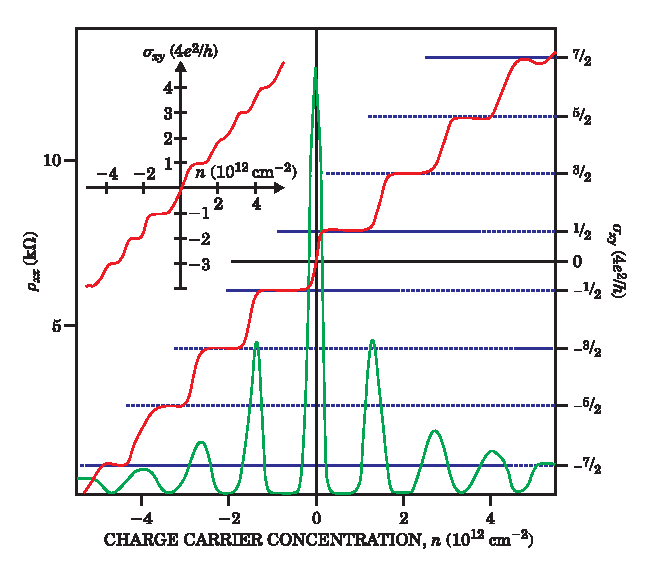
\includegraphics[width=0.7\textwidth]{Drawing/GrapheneQuantumHall.pdf}
	\caption[The quantum Hall effect in graphene]{The quantum Hall effect in graphene. The Hall conductance (red line) follows $\displaystyle \sigma_{xy} = \pm4\left(n + \frac{1}{2}\right)\frac{e^2}{h}$, while the longitudinal resistance (blue line) shows peaks when the Fermi energy transits from one Landau level to another. Adapted from \cite{novoselov2005two}.}
	\label{FIG:GrapheneQuantumHall}
\end{figure}


\chapter{Experimental Methods}
\label{SEC:methods}

\section{Sample growth}

\subsection{LAO/STO growth}
The properties of LAO/STO interfaces is susceptible to growth conditions such as substrate temperature, background oxygen pressure, annealing conditions, etc\cite{cancellieri2010influence}. The samples are grown with pulsed laser deposition (PLD)\cite{bark2011tailoring} by our collaborators, Sangwoo Ryu, Hyungwoo Lee, Jung-Woo Lee, Kitae Eom, and Chang-Beom Eom, at the University of Wisconsin-Madison.

\subsubsection{Pre-growth treatment}

STO (001) substrates are purchased from commercial crystal suppliers. The substrates have a carefully controlled mis-cut angle $< 0.1^{\circ}$, so that the width atomic terraces on STO surface is about 500 nm (Figure \ref{FIG:RHEED}(a)). It has been reported that the terraces on the LAO/STO surface can affect the properties of the LAO/STO interface\cite{fix2011influence}. Before PLD growth, the STO (001) substrates are etched with buffered hydrofluoric acid (HF) to remove SrO and become TiO$_2$ terminated. Then the substrates are annealed at $1000 \ ^{\circ}$C for several hours so that the surface will reconstruct and form crystal terraces\cite{radovic2008low}. 

\subsubsection{PLD deposition}

\begin{figure}[p]
	\centering
	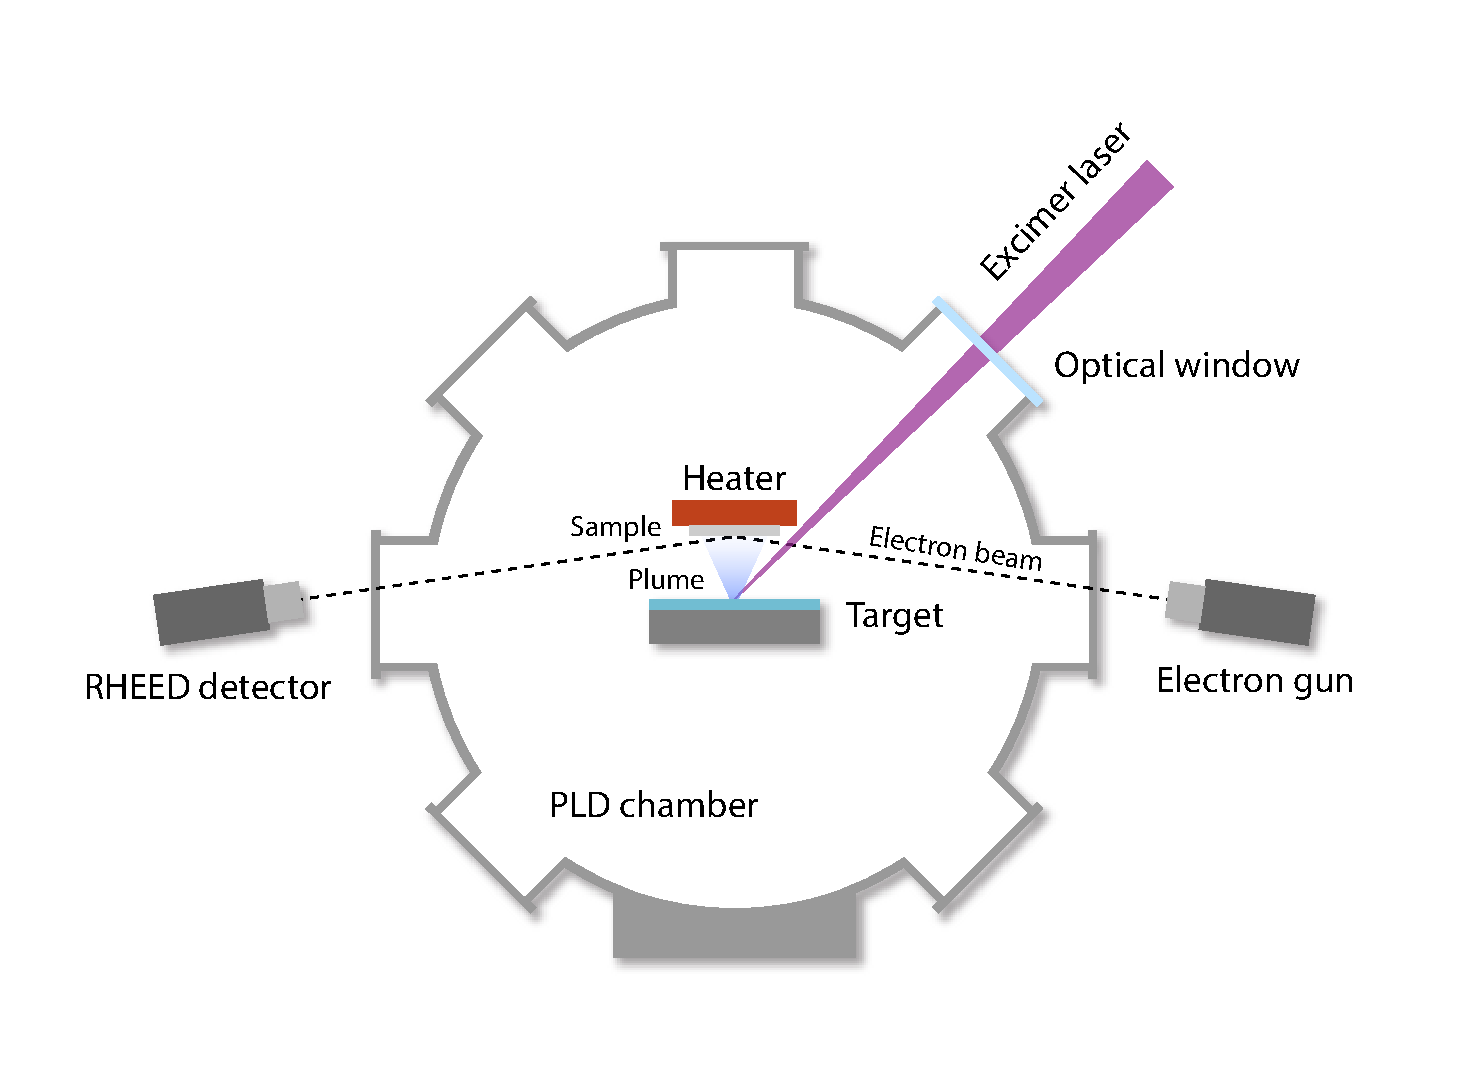
\includegraphics[width=1.0\textwidth]{Drawing/PLD.pdf}
	\caption[PLD epitaxial growth]{PLD epitaxial growth. The PLD chamber is backfilled with oxygen to the target pressure. A beam of pulsed-deep-UV excimer laser is focused onto the LAO target. LAO is ablated off, and a plume of plasma extending towards the heated substrate on top and condensed into atomic layer films. RHEED signal is used to monitor the thickness of LAO.}
	\label{FIG:PLD}
\end{figure}

In PLD deposition, KrF excimer laser ($\lambda = 248$ nm) pulses are focused on a LAO target and plumes of target material are deposited on the pre-heated STO substrates. Two conditions are used for LAO/STO sample growth. (a) STO substrate is heated at $T_\mathrm{STO} = 550 \ ^{\circ}$C and chamber oxygen pressure $P(\mathrm{O}_2)$ is maintained at $1 \times 10^{-3}$ mbar, and sample is annealed in 1 atm of O$_2$ after growth. The samples grown with 3.4 uc thick LAO in this conditions are used for c-AFM writing. (b) STO substrate is heated at $T_\mathrm{STO} = 780 \ ^{\circ}$C and chamber oxygen pressure $P(\mathrm{O}_2) = 7.5 \times 10^{-5}$ mbar; sample is annealed at $T_\mathrm{STO} = 600 \ ^{\circ}$C, $P(\mathrm{O}_2) = 300$ mbar for 1 hour after growth. The samples grown with 12 uc LAO are used for magnetism experiments\cite{bi2014room}.

Figure \ref{FIG:PLD} illustrates PLD epitaxial growth of LAO. The sample is loaded in an ultra-high vacuum chamber, backfilled with oxygen to the target pressure ($10^{-5} \sim 10^{-3}$ mbar). The deep-UV excimer laser is focused on the LAO crystal target through an optical window on the chamber. The target material is ablated off by the laser and forms a plasma plume. The STO substrate is heated up and placed on top of the target. As the plume expands, target material would condense on the substrate and forms atomic-thin films epitaxially. The high temperature of the substrate facilitates crystallization and epitaxial growth of the target material. 

\begin{figure}[hp!]
	\centering
	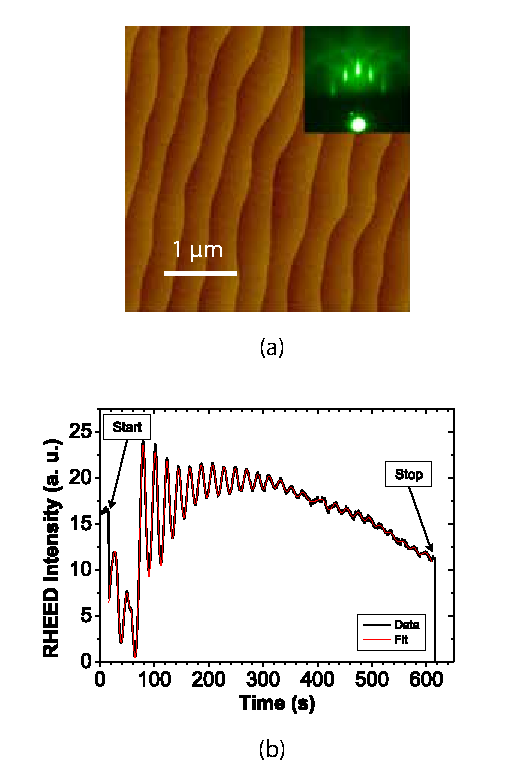
\includegraphics[width=0.65\textwidth]{Drawing/PLD_RHEED.pdf}
	\caption[AFM image of an LAO/STO sample]{AFM image of an LAO/STO sample after PLD growth and RHEED signal for PLD. (a) AFM Image of an LAO/STO sample. The stripes are the crystal terraces, with $h \approx 4 \ \mathrm{\AA}$. Inset of a is the raw diffraction signal of RHEED. (b) RHEED intensity oscillation during the film epitaxial growth. Each cycle indicates the completion of one unit cell. Adapted from \cite{podkaminer2016real}.}
	\label{FIG:RHEED}
\end{figure}

During the PLD growth, the reflection high-energy electron diffraction (RHEED) is used for \emph{in-situ} monitoring the thickness of epitaxial layers. A beam of electron is generated from a source and reflected from the substrate as the film growth. Electron diffraction signal is collected by a detector on the other side (Figure \ref{FIG:RHEED}(a) inset). The intensity of the diffraction oscillates as a function of film thickness. The thickness of LAO can be precisely controlled by counting the cycles of the RHEED signal (Figure \ref{FIG:RHEED}(b)).

\subsection{Graphene growth}

The graphene growth is in collaboration with Shonali Dhingra, Jen-Feng Hsu, and Brian D'Urso from University of Pittsburgh. The growth parameters are from Shonali Dhingra's Ph.D. dissertation\cite{dhingra2015quadratic}.

The two most popular methods to obtain single-layer/few-layer graphene are mechanical exfoliation\cite{novoselov2004electric} and chemical vapor deposition (CVD)\cite{kim2009large}. The mechanical exfoliation isolates single-layer graphene directly with adhesive tapes. Graphene is a type of van der Waals material, where the carbon atoms within a layer are tightly bonded with covalent bonds while the layers are bonded by the much weaker van der Waals force. Adhesive tapes can easily separate graphene layers. After multiple exfoliation steps, single layer graphene flakes can be isolated and identified\cite{novoselov2004electric}. One key aspect of the exfoliation method is choosing a proper substrate so that single-layer graphene can be easily identified with optical microscopes. Although graphene has the highest absorption coefficient in the visible light regime\cite{nair2008fine}, identifying a single layer graphene flake on a transparent substrate is still challenging, and is always assisted with other characterization methods such as Raman spectroscopy\cite{ferrari2006raman}. Silicon wafers with 400 nm thick oxide are commonly used for helping graphene transfer. Graphene with different thickness on silicon oxide substrates would have different colors due to interference.

CVD is another method to obtain single layer graphene\cite{kim2009large}. Graphene flake from mechanical exfoliation is mostly a few micrometers or tens of micrometers; the size and shape cannot be well controlled. CVD method, on the other hand, can grow wafer size graphene\cite{lee2010wafer}, and then the graphene can be transferred and etched into any desired shapes through post-processing. The CVD process uses gaseous organic molecules (methane, ethylene, etc.) as carbon sources, and graphene lattice-matching crystals such as SiC, Ni and Cu are used as substrate. In high temperature ($\sim$ 1000 $^{\circ}$C), the metal surface are highly reactive and can catalyze the formation of graphene. CVD is a dynamic process of etching and growth. Hydrogen molecules can etch away the smaller domains while the larger domains are growing\cite{vlassiouk2011role, zhang2012anisotropic} until the domains are in contact with each other or the gas flow is terminated. If the hydrogen portion is too high, the larger graphene domains will also be etched. The ratio of methane and hydrogen need to be carefully controlled.

\begin{figure}[h!]
	\centering
	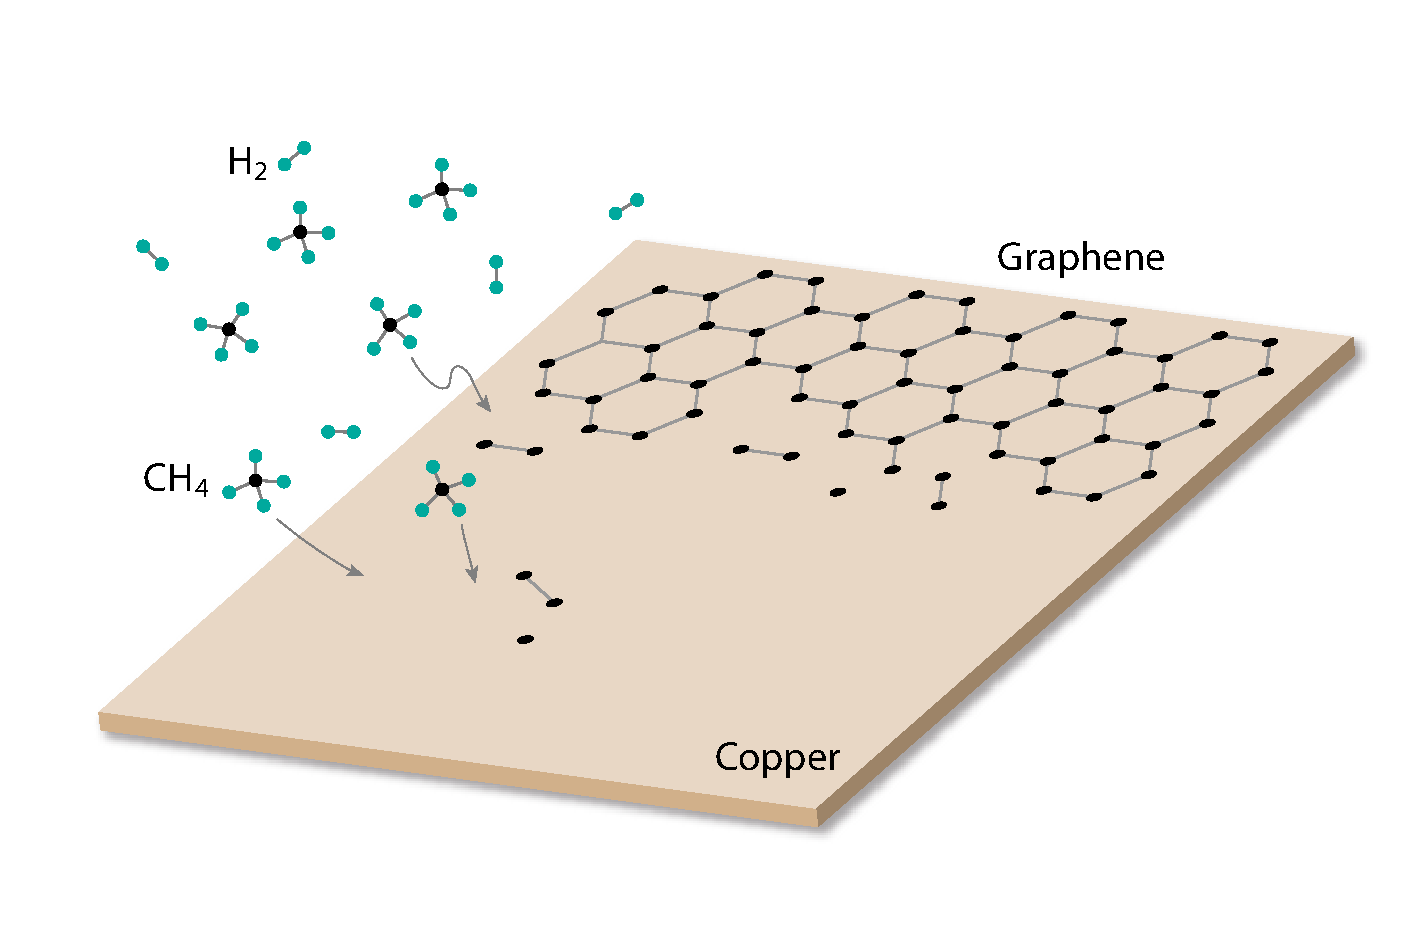
\includegraphics[width=.80\textwidth]{Drawing/CVD.pdf}
	\caption[Graphene CVD growth]{Graphene CVD growth. At a temperature $T \approx$ 1000 $^{\circ}$C, methane molecules will react with copper and leave carbon atoms on the surface. The atoms will self-assemble into graphene due to lattice-match between graphene and copper super-cells. Hydrogen is used to etch away the smaller domain so that the final single layer graphene domains are as large as possible. If the hydrogen is too much, the larger domain will be etched as well. The ratio of methane and hydrogen has to be carefully controlled.}
	\label{FIG:CVD}
\end{figure}

\subsubsection{Copper substrate preparation}

Various materials are used for graphene growth, most commonly SiC, Cu, Ir, and Ni. Cu is the most common choice due to the low carbon solubility\cite{Bae2010}. Compared to other substrate materials, copper is also easy to be etched with wet chemicals. In CVD growth, the carbon atoms form into graphene following the topography of the substrate. Therefore, graphene quality is directly related to the flatness and cleanness of the substrate. Surface contaminants on copper provide nucleation centers for graphene and can cause polycrystalline structure and multi-layer growth\cite{eres2014cooperative}. The issue of surface roughness can be addressed with electrochemical polishing\cite{Bae2010} or mechanical polishing. In this research, graphene substrate are polished using procedures developed by Shonali Dhingra, Jen-Feng Hsu from Dr. Brian D'Urso's group in University of Pittsburgh. The roughness of the copper substrate is reduced from several hundred of nanometer to a few nanometers\cite{dhingra2015quadratic} using a diamond turning machine (DTM). Compared to electrochemical polishing, this method can produce surfaces that are 50 times smoother, and the copper domain sizes are five times larger\cite{dhingra2014chemical}. 

DTM is used for high precision manufacturing, such as laser reflective mirrors. The machine works like a lathe, where the workpiece is fixed on a turning spindle, and the cutting tool approaches the workpiece and shape or polishes the surface by steps. Figure \ref{FIG:DTM} shows the DTM in operating. The cylindrical metal piece in Figure \ref{FIG:DTM}(a) is the spindle of DTM. The copper piece is attached to the spindle by vacuum and spins at 2000 rpm. The diamond tool approaches the copper surface from the opposite side. Figure \ref{FIG:DTM}(b) is an image taken in the middle of a cutting step. Mineral spirit is sprayed from a nozzle from the left, cools down the surface and blows away the metal debris to the right. Reflection of the tool shows a smooth finishing.

\begin{figure}[h!]
	\centering
	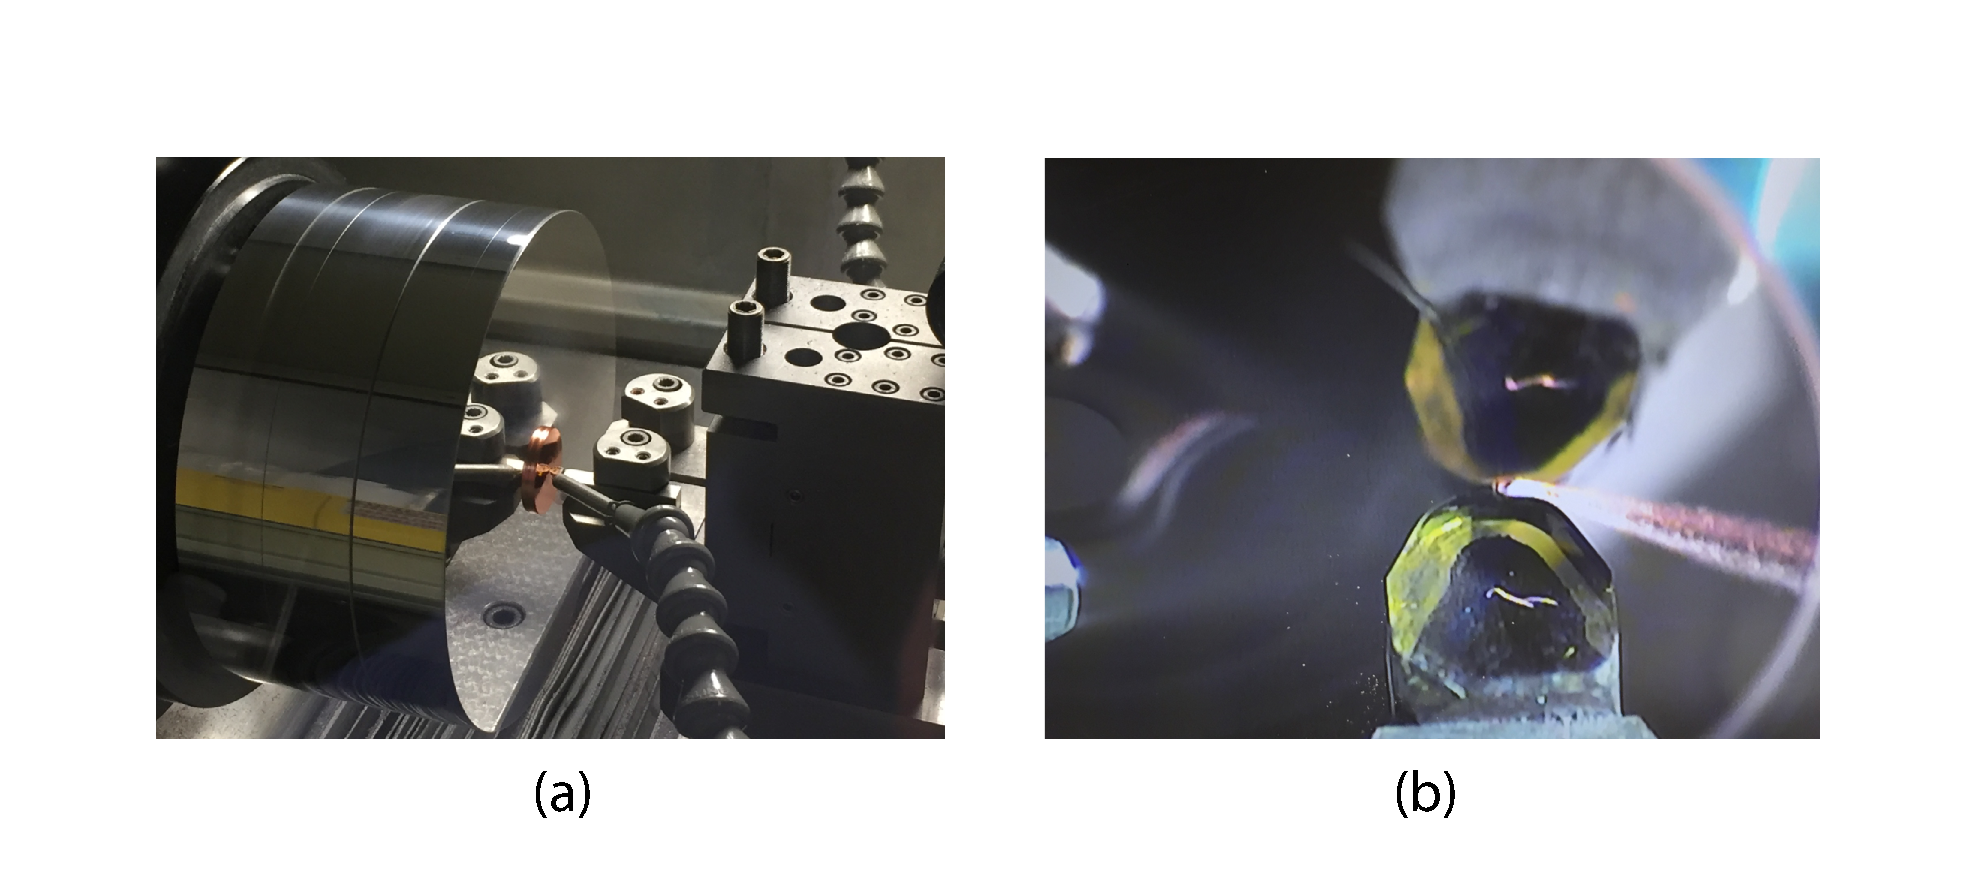
\includegraphics[width=1.0\textwidth]{Drawing/DTM.pdf}
	\caption[Diamond turning machine at work]{Diamond turning machine at work. (a) Copper is fixed onto a turning spindle with vacuum. (b) Mineral spirit is sprayed to the tool and cutting spot, to cool down the surface and blow away the debris.}
	\label{FIG:DTM}
\end{figure}

The DTM uses a curved-edge (radius of curvature $r$ = 1.5 mm) diamond tool for cutting (Figure \ref{FIG:DiamondTool}). By reducing the incremental step to 10 $\mu$m, the roughness of the finishing surface can be smaller than 2 nm (Figure \ref{FIG:DTMFinishing} (b)). The diamond tool sometimes has dents on the surface, which can leave traces after each revolution.

\begin{figure}[h!]
	\centering
	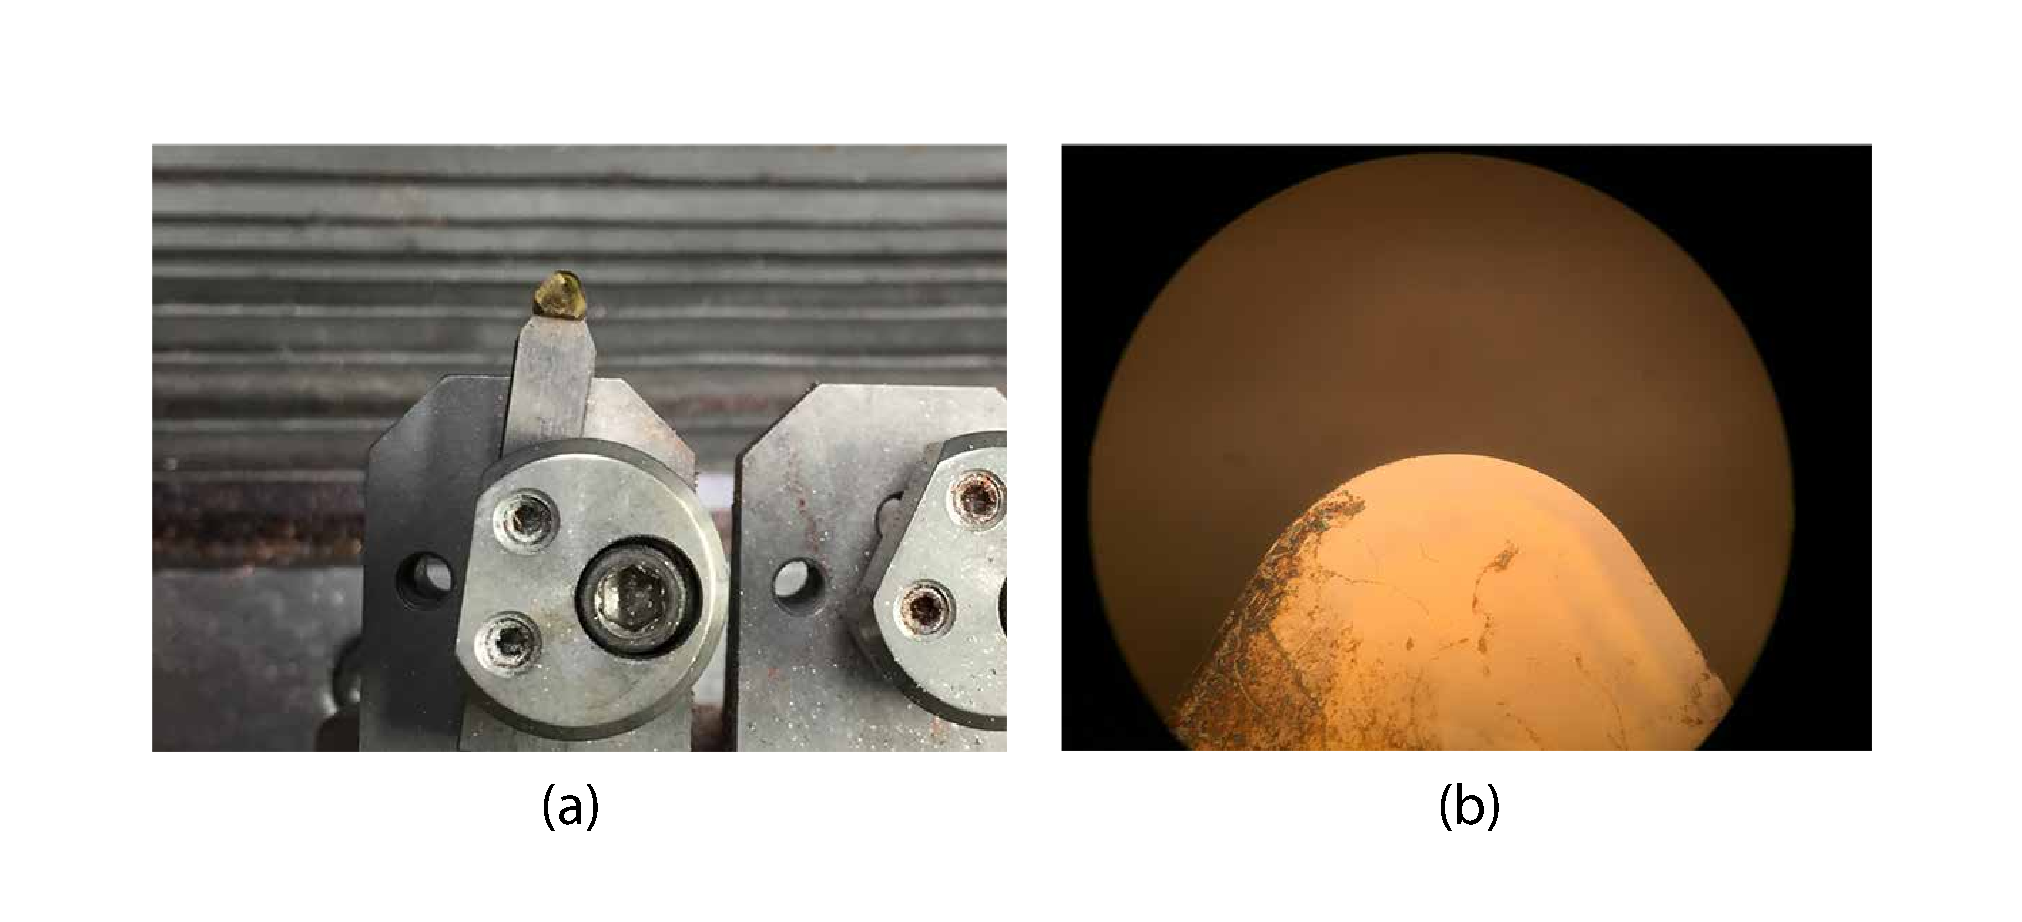
\includegraphics[width=1.0\textwidth]{Drawing/DiamondTool.pdf}
	\caption[Images of the diamond tool]{(a) Diamond cutting tool. (b) Magnified image of the tool tip. The radius of curvature $r = 1.5$ mm.}
	\label{FIG:DiamondTool}
\end{figure}

\begin{figure}[h!]
	\centering
	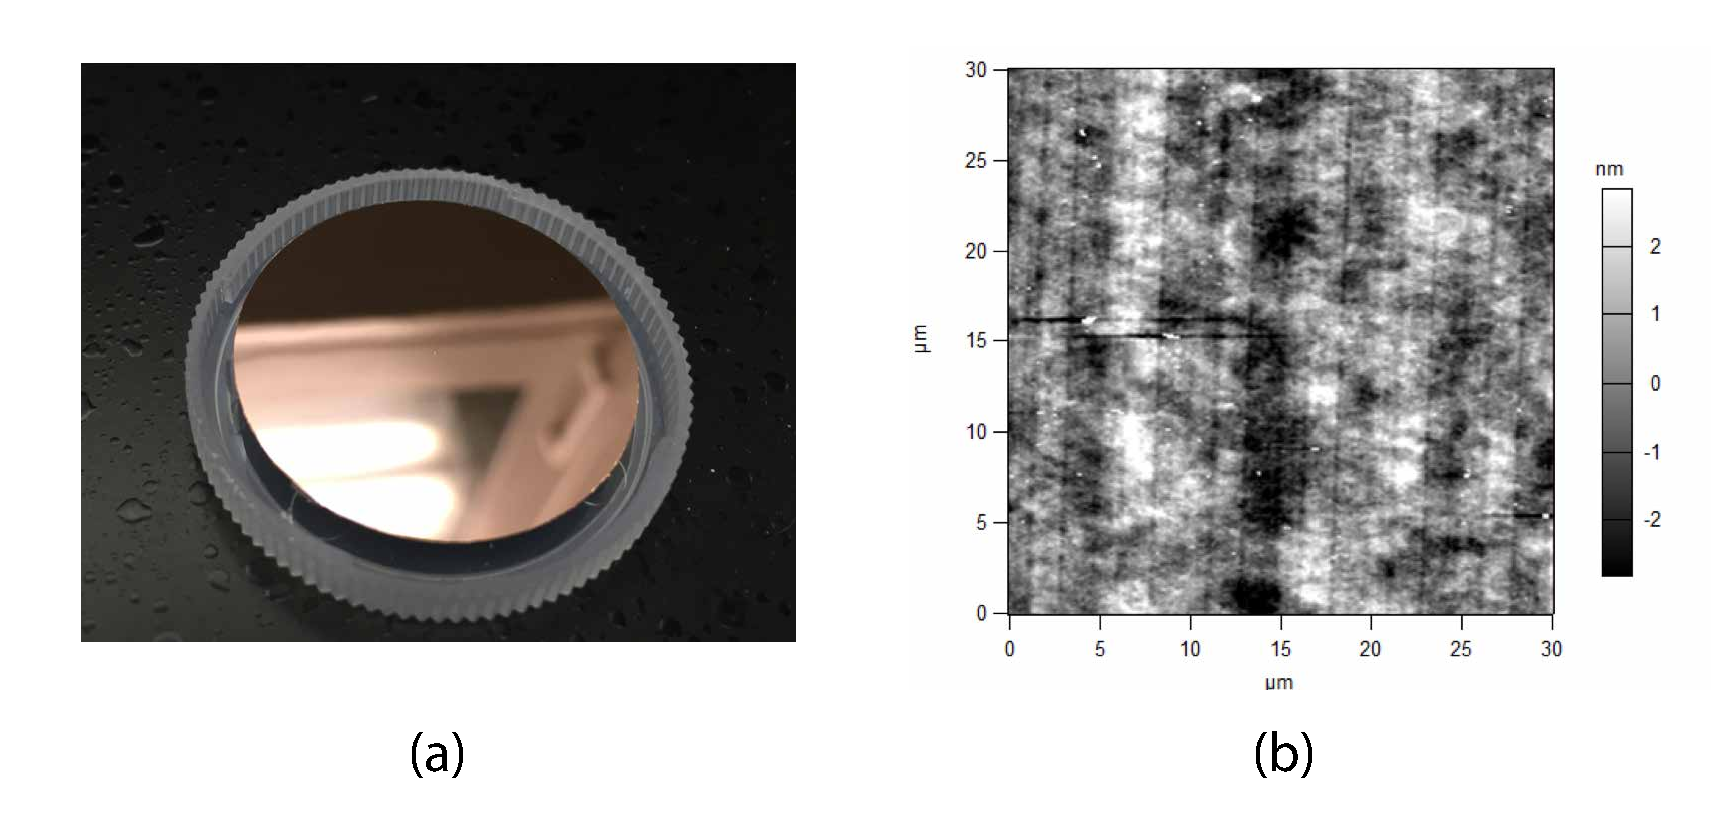
\includegraphics[width=1.0\textwidth]{Drawing/DTMCopper.pdf}
	\caption[Copper substrate after DTM cutting]{Copper substrate after DTM cutting. (a) The reflective copper surface after DTM polishing. The final thickness of the substrate is about 100 $\mu$m. (b) The AFM image of the copper foil surface. The roughness is within 2 nm. Some nanoscale particles can be seen. Reducing the density of surface contaminants will reduce the density of nucleation centers and enlarge the domain size. The vertical grooves are left by the dents on the diamond tool for each revolution. The copper is annealed at $T = 1050$ $^{\circ}$C for another time before the growth starts, and the surface will reconstruct and groves are flattened.}
	\label{FIG:DTMFinishing}
\end{figure}

Other than surface roughness, the copper domain size is another limiting factor for sizeable single domain graphene growth. Although it was not clear the effect of copper substrate domains on the graphene quality\cite{kim2012direct, wang2012controllable, wofford2010graphene}, larger copper domain sizes give us a chance to grow larger graphene single crystals. Annealing the copper at high temperature will reconstruct and merge the polycrystalline domains into larger domains, but mechanical processing will introduce defects and break the single domains; therefore the substrate needs to be re-annealed before graphene growth starts.

\begin{figure}[p]
	\centering
	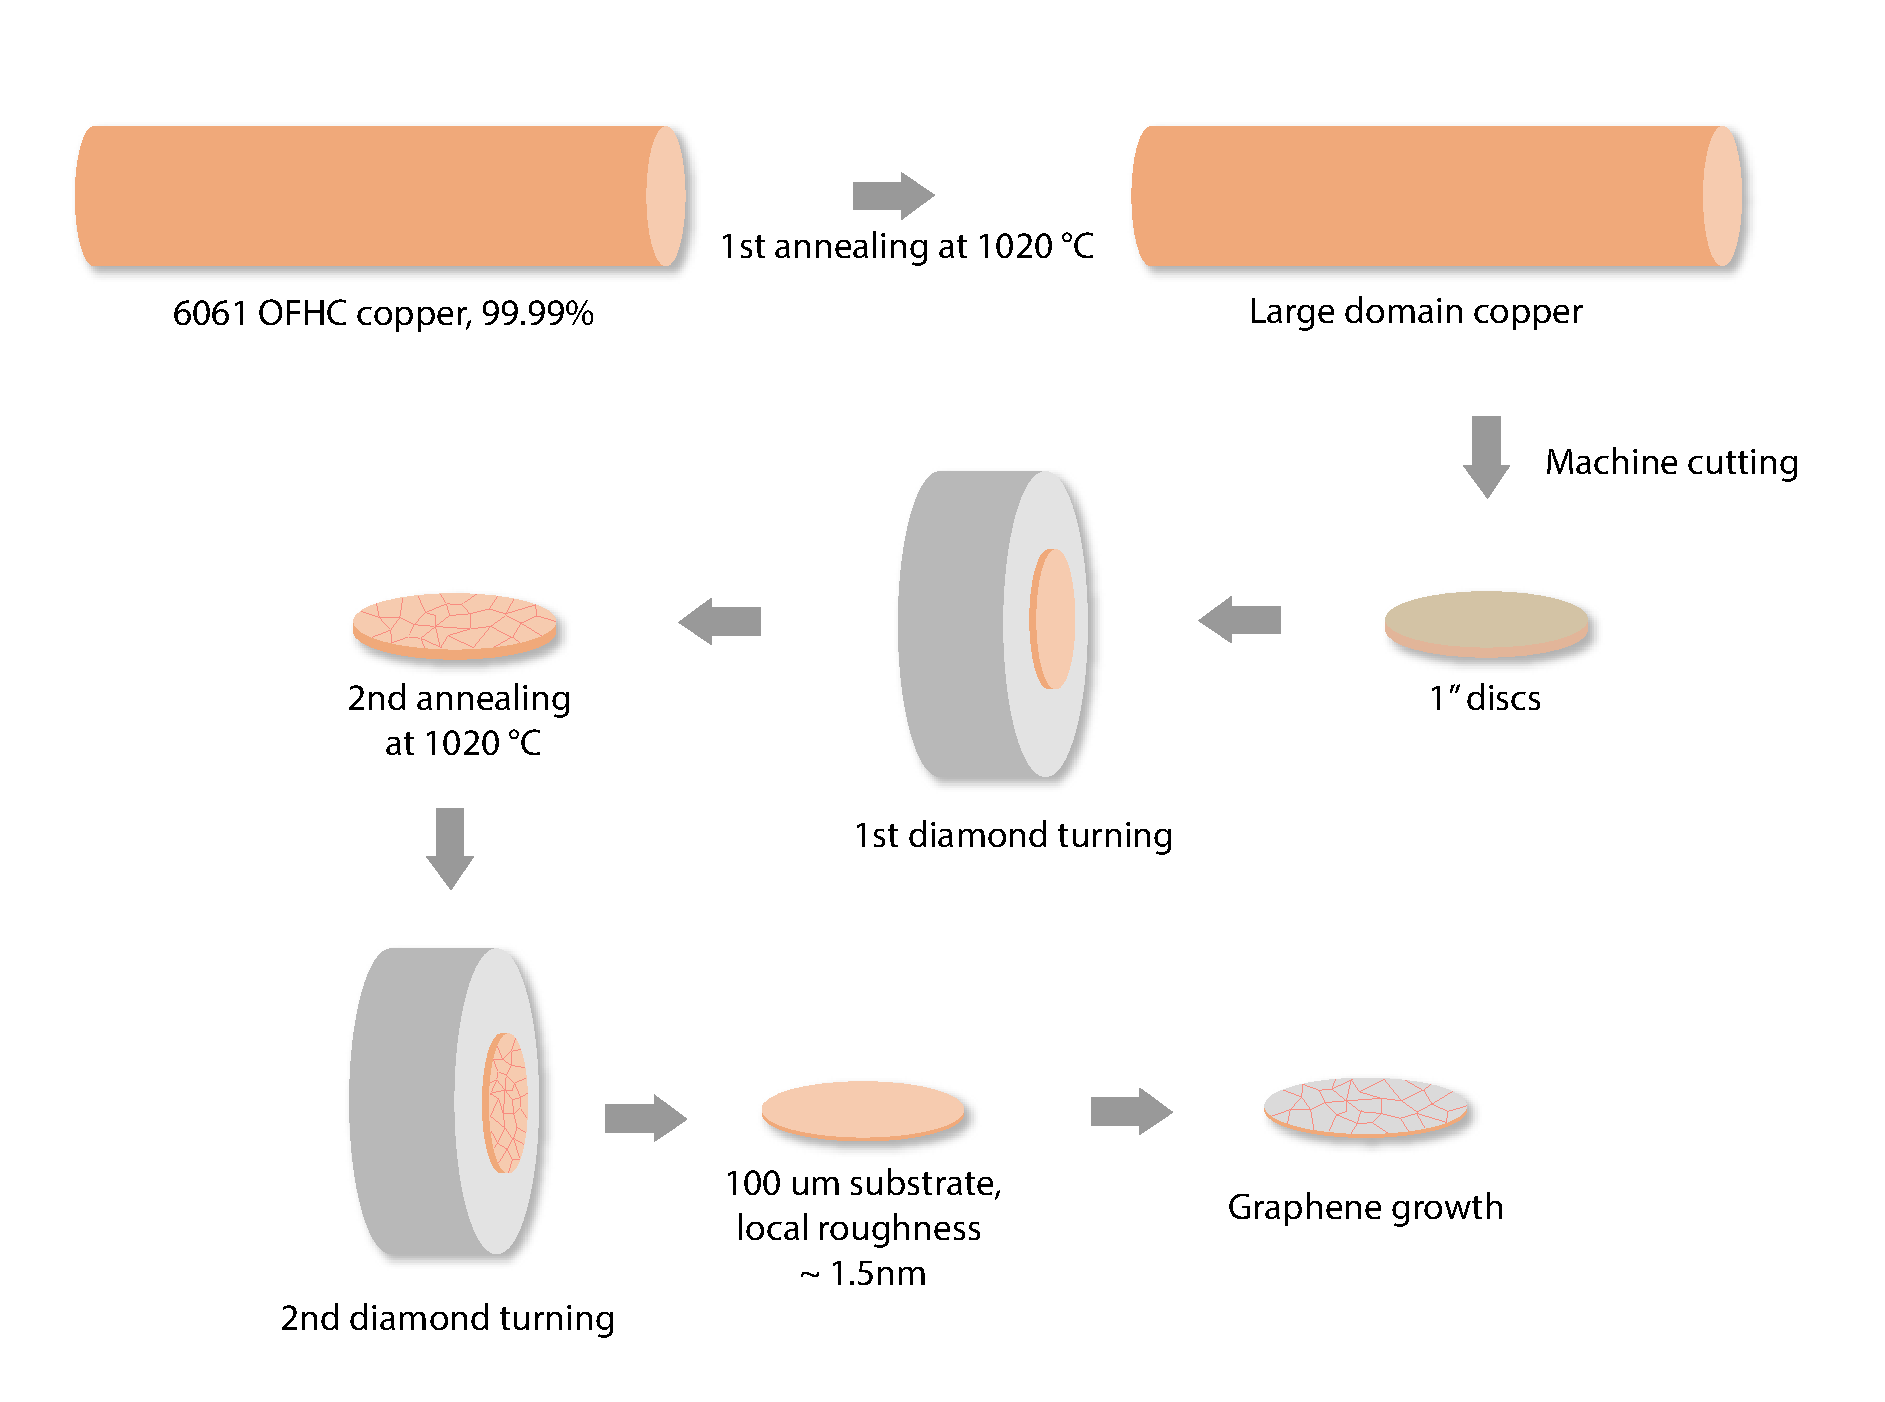
\includegraphics[width=1\textwidth]{Drawing/CopperProcessing.pdf}
	\caption[Procedure of copper substrate preparation]{Procedure of cutting copper rods into 100 $\mu$m foils for graphene growth. High purity OFHC copper rods are purchased from McMaster Carr. The rod is first annealed at 1050 $^{\circ}$C for 24 hours so that the polycrystalline domains merge into larger domains. Then the rod is cut into 2 mm thick copper discs in the machine shop. The discs are cleaned with DTM and then annealed again to ``heal'' the domains broken by the mechanical cutting. Domain re-formation would cause surface corrugation. Thus, the copper disc surface is cleaned with DTM and then cut into 100 $\mu$m foils.}
	\label{FIG:CopperProcessing}
\end{figure}

The procedure of making copper rods into copper foils for graphene growth is shown in Figure \ref{FIG:CopperProcessing}. 1' long oxygen-free high thermal conductivity copper (OFHC) rods with ultra-high purity (99.99\%) are purchased from McMaster Carr. The rod is first annealed at $T=1050$ $^{\circ}$C for 24 hours, and the polycrystalline domains in the rod will merge into larger domains within. Then the rod is then cut into copper discs of 2 mm thick in the machine shop. The mechanical cutting process will break the domains and introduce surface contaminant, so the surfaces copper discs are cleaned on the DTM, and then annealed again at 1050 $^{\circ}$C for 8 hours. After annealing, the domain re-formation in the disc will cause corrugation on the surface. Therefore, the copper surface is polished with DTM for a second time. Then the copper discs are cut into 100 $\mu$m foils, by 10 $\mu$m steps.

\subsubsection{CVD growth}

\begin{figure}[p]
	\centering
	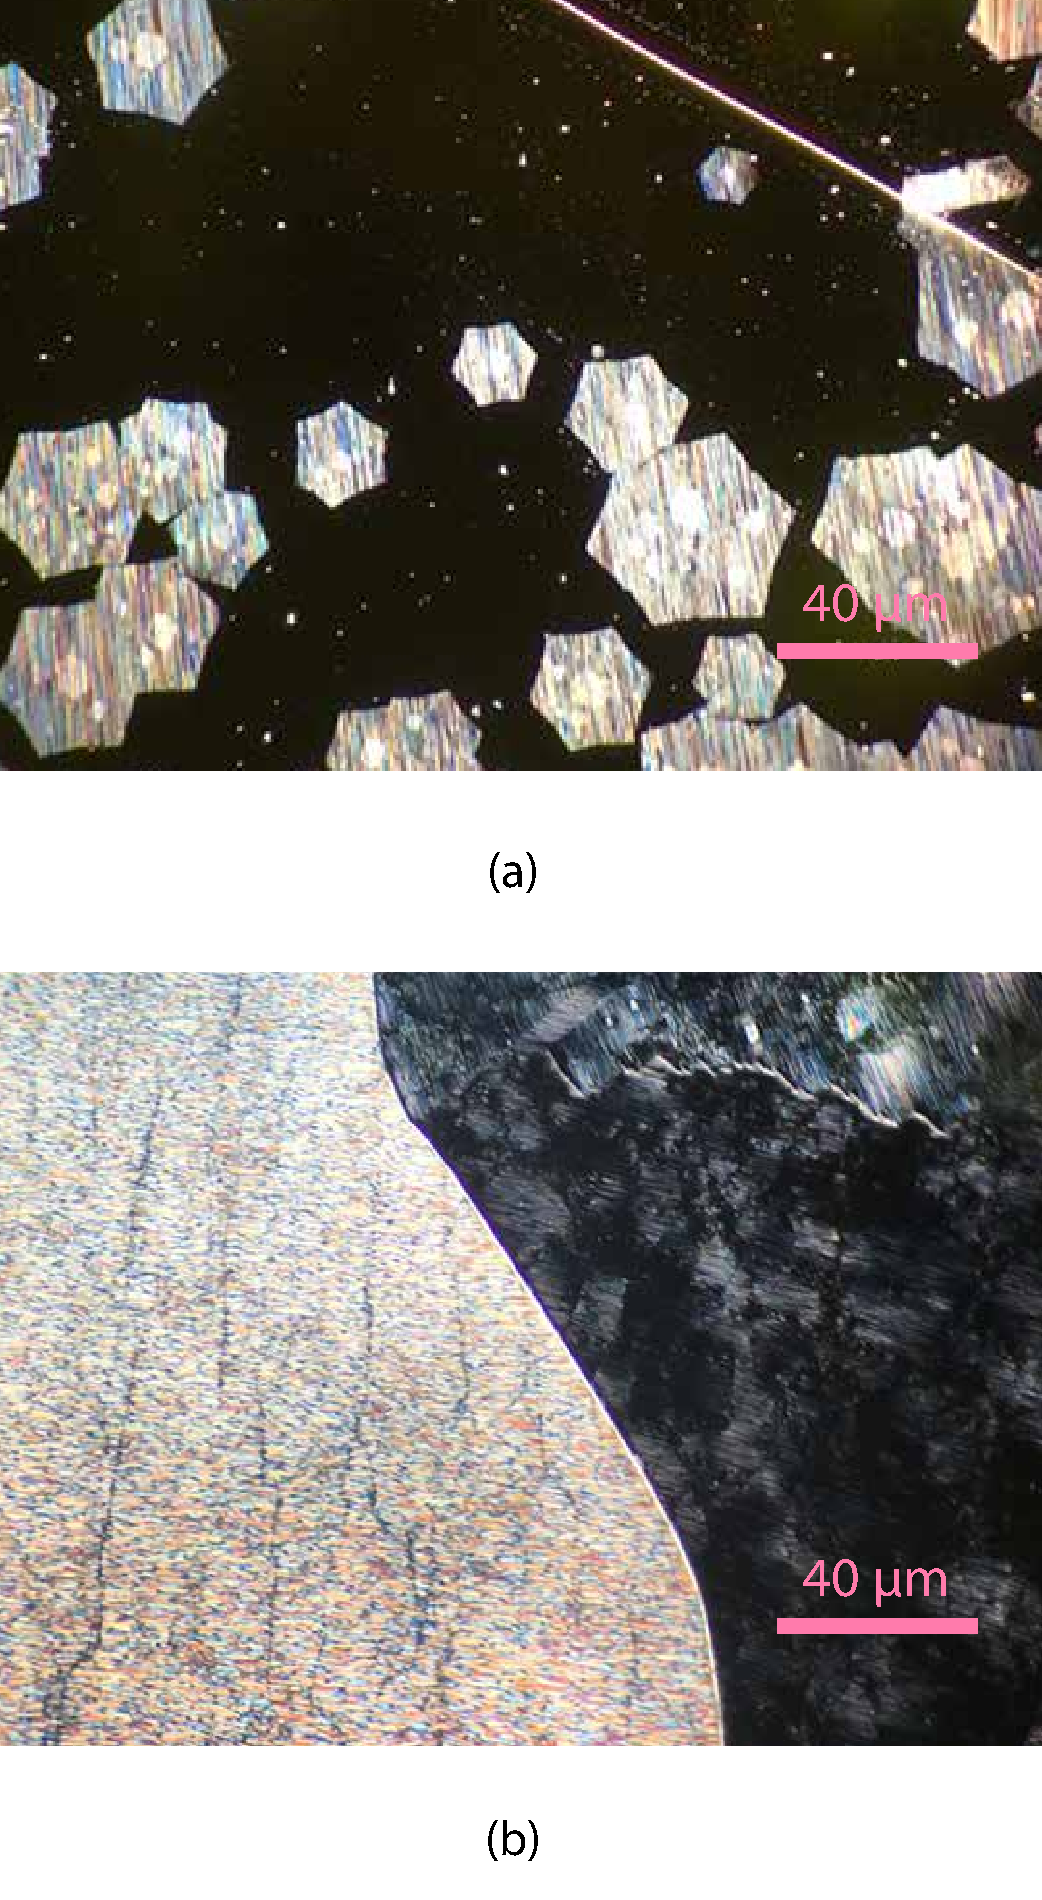
\includegraphics[width=0.6\textwidth]{Drawing/CVDGraphene.pdf}
	\caption[Dark field mode microscope images of CVD graphene on copper substrates]{Dark field mode microscope images of CVD graphene on copper substrates. (a) The copper substrate is partially covered with graphene. Hexagonal shape single domain graphene can be observed. Growth was terminated before graphene fully covered the substrate. (b) Graphene covers the entire copper substrate. Copper domains of two different orientations can be observed.}
	\label{FIG:CVDGraphene}
\end{figure}

The CVD graphene growth can be performed in low pressure (LPCVD) or atmospheric pressure (APCVD). LPCVD grows graphene at a pressure lower than 100 mTorr, in a continuous flow of hydrogen and methane mixture while the substrate is heated to 1000 $^{\circ}$C. The issue with LPCVD is that the melting point of copper ($T_m = 1085^{\circ}$C) is close to the growth temperature. As a result, the copper will evaporate severely and contaminate the furnace\cite{vlassiouk2013large}. Also, pure precursor gases bring fire hazard. APCVD can eliminate those difficulties and improve the graphene quality\cite{vlassiouk2013large, dhingra2015quadratic}. Instead of using pure hydrogen and methane, APCVD uses a gas mixture of 2.5 vol \% H$_2$, 0.1 vol \% CH$_4$, and balance Ar. The furnace is pumped to low vacuum, and then backfilled with the gas mixture to atmospheric pressure. The pressure from argon will suppress the evaporation of copper at high temperature. 

The growth procedures are as follows\cite{dhingra2015quadratic}. 

\begin{itemize}
	\item The furnace is pumped down to $\sim$ 10 mTorr.
	\item Backfill the furnace with H$_2$/Ar mixture at 186 sccm, up to $\sim$ 100 Torr.
	\item Start the furnace temperature controller to ramp up to $T = 1050$ $^{\circ}$C, and let the furnace stay at this temperature for 1 hour.
	\item Start flowing mixture of CH$_4$/Ar at 14 sccm into the furnace and let the copper foil stay in graphene CVD growth condition for 1.5 hours.
	\item Cool down the system to room temperature. The flow of CH$_4$/Ar mixture is turned off at $\sim$ 650 $^{\circ}$C. H$_2$/Ar mixture keeps flowing overnight until the system is below 50 $^{\circ}$C. 
	
\end{itemize}

In Figure \ref{FIG:CVDGraphene} the dark-field mode of optical microscope clearly shows the CVD graphene on copper substrates. In \ref{FIG:CVDGraphene}(a) the copper substrate is partially covered with graphene. The growth process was terminated before graphene entirely covered the substrate. The hexagonal shape of single domain graphene flakes can be identified. Some double layer can also be observed. On the top right corner of \ref{FIG:CVDGraphene}(a) a copper domain boundary can also be identified. \ref{FIG:CVDGraphene}(b) is the image of graphene grown in another run. The substrate is entirely covered with graphene. The picture shows two copper domains with different orientations, and therefore the graphene grown on the two domains look different. Wrinkles on graphene can be observed, resulting from different thermal expansion coefficients of copper and graphene. 

\section{LAO/STO sample processing}

One of the challenges with experiments on the LAO/STO interface is to make good electrical contact from the bonding pads to the interface. A major part of my Ph.D. research is to process the samples for the c-AFM writing, or graphene transfer. The processing methods have to be carefully chosen so that the 2DEG and interface switchability will not be affected. Sample cleanness is another concern. Nano-particles introduced in the processing would affect sample quality, considering that the dimensions of devices are also nanoscale. The LAO/STO sample processing recipe is adapted from the previous work of Daniela Bogorin and Mengchen Huang from University of Pittsburgh.

\begin{itemize}
	
	\item \textbf{Initial cleaning}: the sample is cleaned with acetone and isopropanol alcohol (IPA) in ultrasonic cleaner to remove the surface contaminants. Usage of deionized-water (DI-water) is usually avoided. Proton from the water can get adsorbed on the sample surface and affect the interface writability\cite{xie2011control, brown2016giant, bi2010water}.
	
	\item \textbf{Photolithography}: the sample is patterned with standard UV-photolithography procedures, either with optical masks and a UV-lamp, or with the direct laser writer (DLW). The resolution of the lithography is 2 $\mathrm{\mu}$m.
	
	\item \textbf{Ion milling}: the sample is bombarded with Ar$^+$ ion flow so that the LAO/STO interface is exposed for electrical contact; other regions are protected with the photoresist.
	
	\item \textbf{Deposition}: titanium and gold are used for contact materials to the LAO/STO interface. The metals are deposited by electron-beam evaporation or sputtering.
	
	\item \textbf{Lift-off}: the step removes the excessive metals covering the photoresist. IPA and acetone are used as photoresist solvents and the excessive metals are detached by the ultra-sonic cleaner.
	
	\item \textbf{Oxygen plasma cleaning}: the contaminants introduced by the processing are cleaned with oxygen plasma cleaner. Then the atomic steps can be observed with AFM afterwards.
	
\end{itemize}

\subsection{Photolithography}
\label{SEC:Photolithography}

The substrate is covered with a thin layer photoresist and exposed to UV with designed patterns. UV changes the solubility of photoresist, and the exposed pattern can be developed in a buffered-base solution. There are factors for the resolution of photolithography: diffraction limit of light and photoresist thickness. The modern state-of-the-art photolithography technology can reach a resolution of 10 nm and is the building block of the semiconductor industry. There are two types of photoresists: positive and negative. Positive photoresist is be washed off after been exposed to UV, while negative photoresist is stabilized by UV and developer remove the unexposed parts. In this research, three types of positive photoresists (AZ4620, AZ4210, and AZ4110) are used for different purposes. 

\subsubsection{Spin-coating}

 Spin-coating is the standard technique to cover the sample uniformly with photoresists. When the sample is spinning between 1000 rpm and 6000 rpm, the photoresist solution on the sample surface will spread out. The liquid will be in an equilibrium of viscosity, roughness of sample surface and centrifugation from spinning. After the spin-coating, the sample is baked at a temperature around 100 $^{\circ}$C to vaporize the remaining solvent in the photoresist and stabilize the film before UV exposure. In this research, the spinning speed is 4000 rpm. The thickness of AZ4210 and AZ4110 are 2.1 $\mu$m and 1.1 $\mu$m, respectively. These two types of photoresists have the same chemical composition, but different concentrations, so they will end up with different thickness at the same speed. Usually, thinner films will have more stable performances for small features.

The spin-coating recipes are listed in Table \ref{TAB:photoresistsCoating}.

\begin{table}
	\centering
	\begin{tabular}{l|cc}
		\hline
		Photoresist    &    AZ4210    &    AZ4110 \\ \hline
		Spinning speed    &    4000 rpm    & 4000 rpm    \\ 
		Spinning time    &    30 s    &    30 s    \\
		Baking temperature    &    95 $^{\circ}$C    &    95 $^{\circ}$C \\ 
		Baking time    &    60 s    &    60 s    \\
		Thickness    &    2.1 $\mu$m    &    1.1 $\mu$m \\ \hline
	\end{tabular}
	\caption{Spin-coating conditions for AZ4210 and AZ4110}
	\label{TAB:photoresistsCoating}
	
\end{table}

\subsubsection{UV exposure}

The UV exposure is to use photon to change the solubility of the photoresist so that the developing step can selectively remove the photoresist. Like all optical system, the resolution of exposure is limited by the diffraction limit of light. Mercury gas-discharge lamp or solid state lasers are used as UV sources. Samples are exposed with two different methods: mask exposure and direct laser writing. 

Mask exposure is performed by a mask aligner (Suss MJB3 or MA6, see Figure \ref{FIG:Suss}). Incoherent and collimated UV is generated from a Hg lamp. The sample is exposed to UV at a constant intensity of 10 mW/cm$^2$, while being covered with a photomask (Figure \ref{FIG:MASK}). Photomask is a square piece of soda glass (to reduce UV absorption) coated with chromium on one side. The designed pattern is pre-printed to the chromium side by chemical etching.

\begin{figure}[h!]
	\centering
	\vspace{0.85cm}
	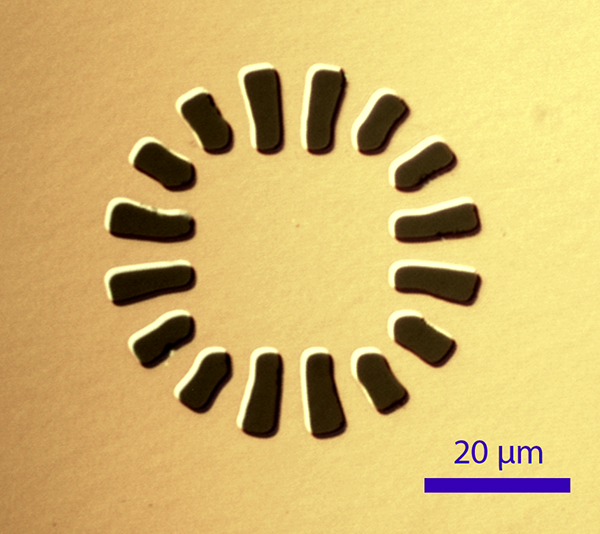
\includegraphics[width=0.4\textwidth]{Drawing/MASK.png}
	\caption[Mask for photolithography]{Mask for photolithography. The dark regions are transparent, while the bright regions are covered with chromium. The sample is be exposed where UV is not blocked by chromium. The figure shows the electrodes of a canvas for c-AFM writing.}
	\label{FIG:MASK}
\end{figure}

\begin{figure}[hp!]
	\centering
	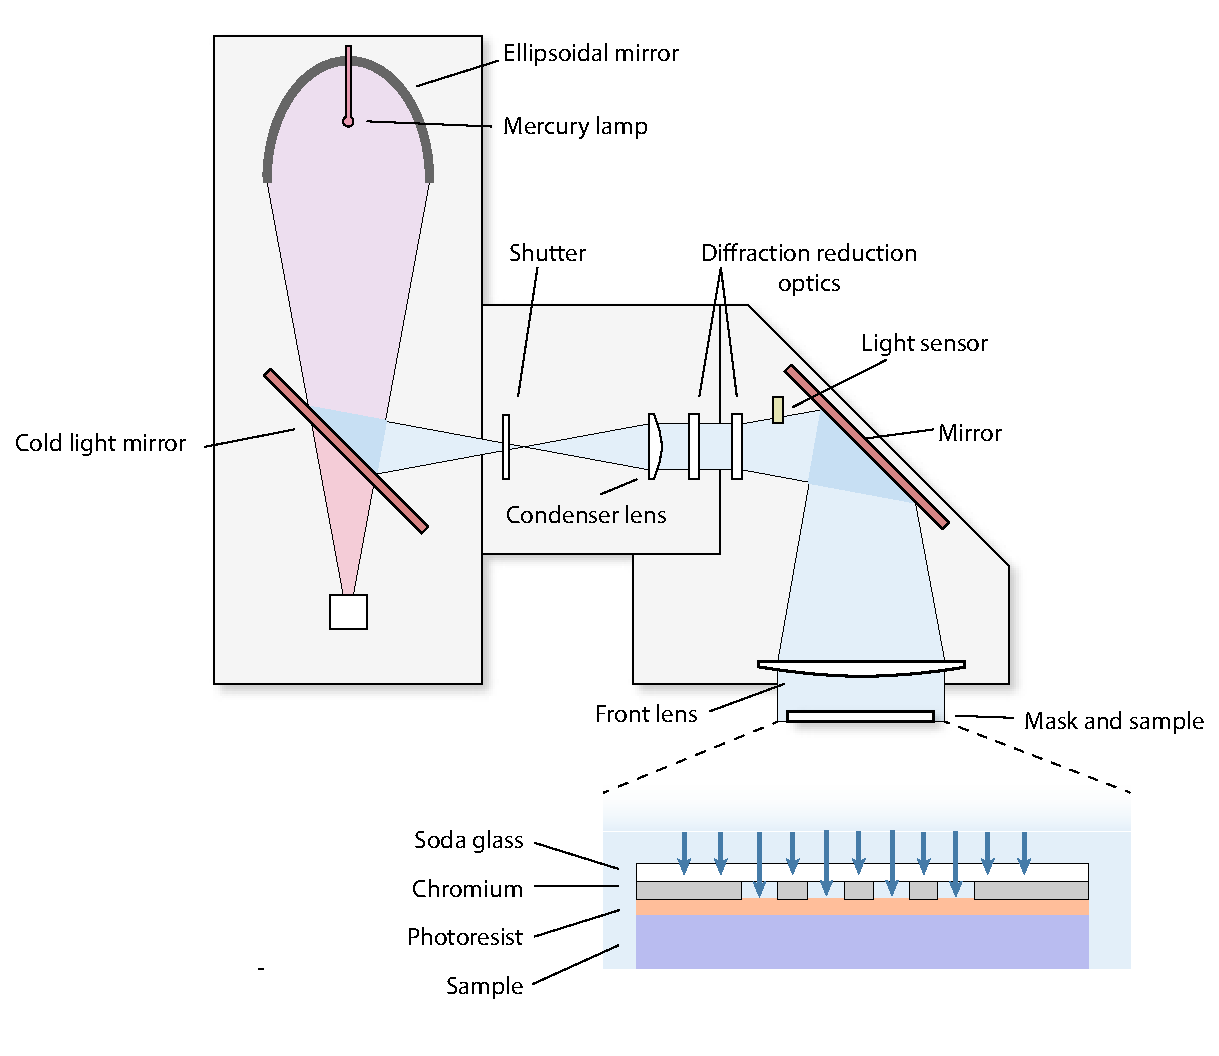
\includegraphics[width=1.0\textwidth]{Drawing/Suss.pdf}
	\caption[Suss UV mask aligner]{Suss UV mask aligner. The mercury lamp generates broadband light from the arc. The light is reflected by an ellipsoidal mirror and focused on a cold light mirror, where the UV is selected. A shutter controls the exposure time and dose. The UV is collected by a condenser lens and diffraction reduction optics for collimation and resolution enhancement. Finally, the UV is shed on the sample with a folding mirror and front lens. The sample is in close contact with a mask, where chromium is partially removed. UV exposes the photoresist on the sample and print the mask pattern on it.}
	\label{FIG:Suss}
\end{figure}

\begin{figure}[hp]
	\centering
	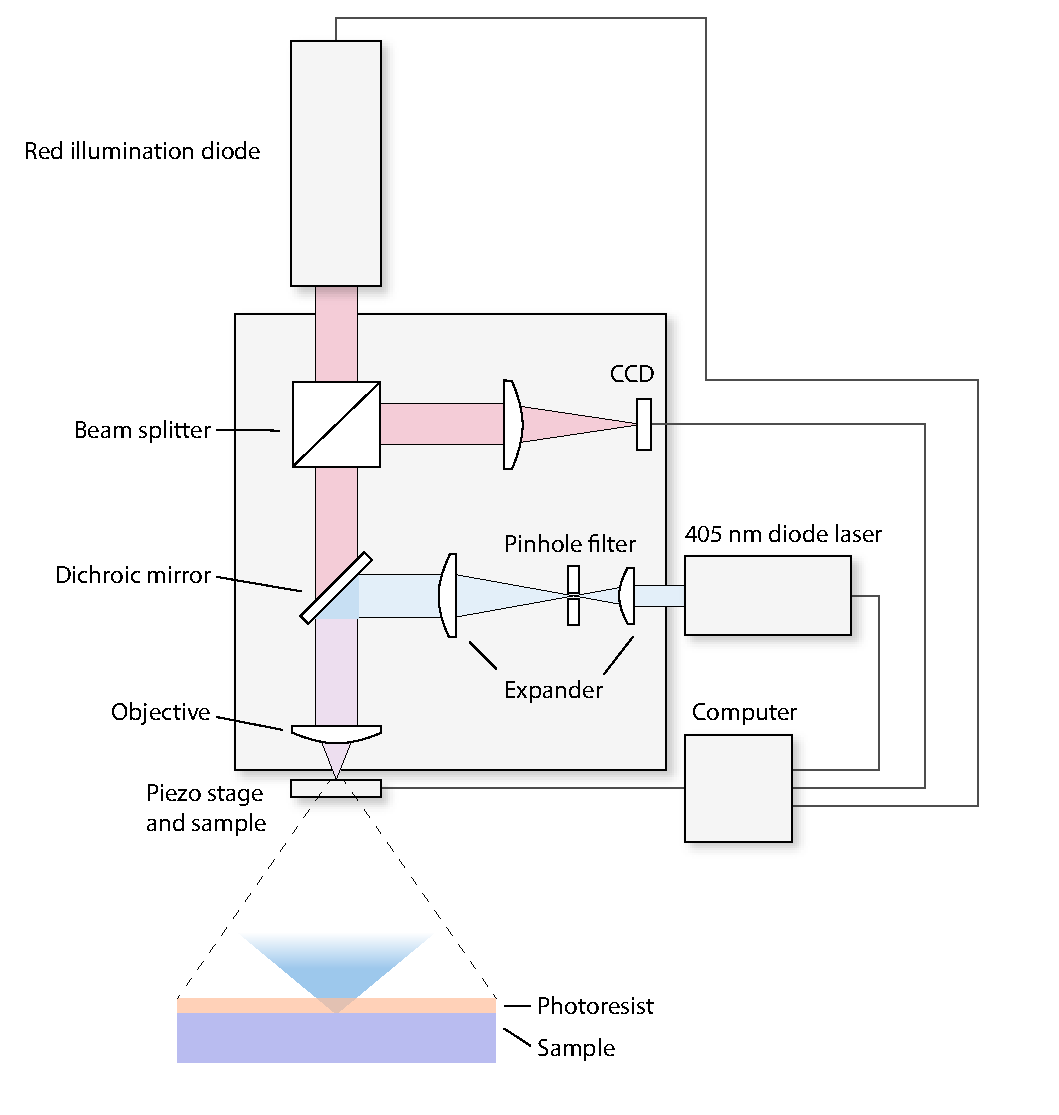
\includegraphics[width=1.0\textwidth]{Drawing/Heidelberg.pdf}
	\caption[Heidelberg direct laser writer]{Heidelberg direct laser writer. The sample is illuminated by red light from a diode, and a real-time image of the sample surface can be monitored with a CCD. UV with $\lambda=405$ nm is generated from a laser diode. The laser is expanded and filtered and focused on the sample surface with a high-NA objective. The sample is fixed on a piezo-driven stage. The CCD image, laser power, sample movement, and layer alignment are all controlled with a computer so that the laser path and dose control is fully automatic.}
	\label{FIG:Heidelberg}
\end{figure}

DLW uses a focused laser beam to write micro-patterns directly on the photoresist. In this research, 405 nm wavelength UV laser generated from Heidelberg MLA100 (Figure \ref{FIG:Heidelberg}) DLW. The laser is expanded and filtered with a pinhole and focused on the sample with a high-NA objective. The focusing objective is fixed, and the sample is placed on a piezostage controlled with a computer. The UV dose is determined by both the laser power and laser spot dwelling time. It is essential to keep the sample surface horizontal so that the laser spot will not defocus while moving through the entire sample surface. 

\subsubsection{Developing}

Developing is the process using buffered base solution to wash away the unwanted parts of photoresist after exposure. Depending on the type of photoresist, either the exposed regions (positive photoresist, such as AZ4210) or unexposed regions (negative photoresist, such as AZ5214) are removed. In this research AZ400K (potassium borate) is used for developing. The developer is diluted with DI-water, by 1:3 or 1:4 ratio; different concentration will maintain different pH level and developing speed. The sample is washed with DI-water after developing, to remove the excessive developer. 

An image of the sample after UV exposure and developing is shown in Figure \ref{FIG:Developed}. The photoresist in the bright area are washed away while the rest of the sample is still covered with photoresist. The conditions for exposure and developing are listed in Table \ref{TAB:photoresistsExposureDeveloping}.

\begin{figure}[h!]
	\centering
	\vspace{0.85cm}
	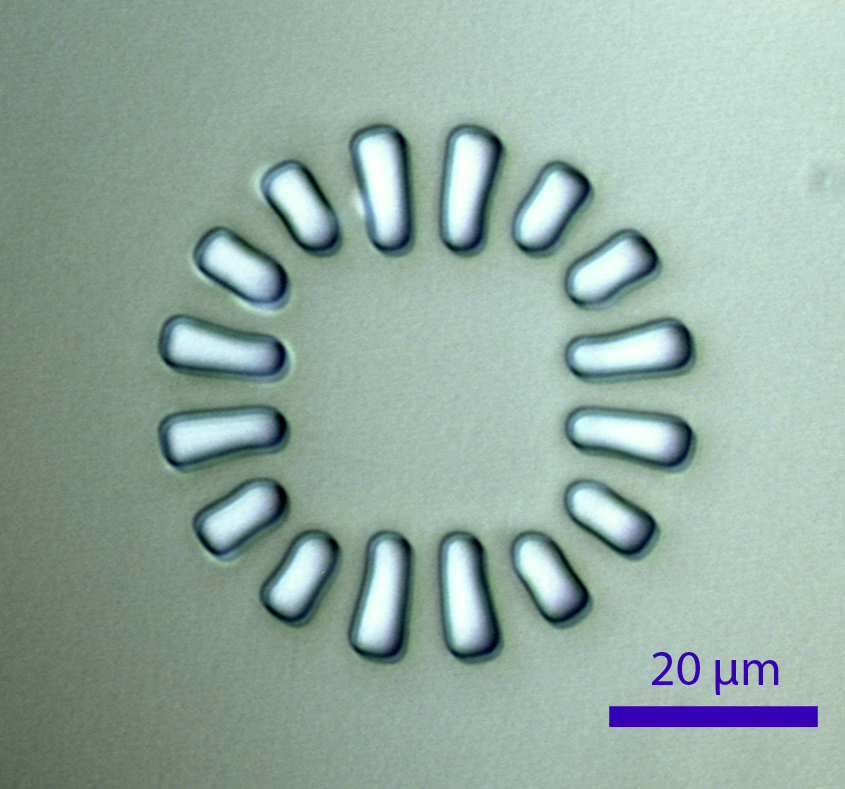
\includegraphics[width=0.4\textwidth]{Drawing/Developed.png}
	\caption[Exposed and developed sample]{Exposed and developed sample. The bright regions are free of photoresist while the rest of the sample is still covered.}
	\label{FIG:Developed}
\end{figure}

\begin{table}[h!]
	\centering
	\vspace{0.85cm}
	\begin{tabular}{l|cc}
		\hline
		Photoresist    &    AZ4210    &    AZ4110 \\ \hline
		UV Dose    &    170 mJ    & 100 -- 120 mJ    \\ 
		Developer : Water    &    1 : 4    &    1 : 4    \\
		Developing time    &    120 -- 180 s    &    120 -- 180 s \\ 
		Resolution    &    3 -- 5 $\mu$m    &    2 $\mu$m    \\ \hline
	\end{tabular}
	\caption{UV exposure and developing conditions for AZ4210 and AZ4110}
	\label{TAB:photoresistsExposureDeveloping}    
\end{table}

\subsection{Ion milling}
\label{SEC:IonMilling}
LAO/STO interface is buried underneath LAO. When making contact the interface, the LAO needs to be etched. Usually, there are three methods for etching: wet-chemical etching, plasma etching, and ion milling. Wet-chemical etching using reactive chemical solutions (such as HF, HCl) to etch away the materials. The process is less expensive but is also less controlled. Plasma etching utilizes the plasma or free radicals of active gas molecules (such as O$_2$, SF$_6$, etc.) to react with the materials, at a pressure between 0.1 and 5 Torr. RIE is better controlled in etching rate and directionality, but the instrument is more expensive. Finding the right gas to selectively etch the target material while keeping the protecting layer intact is not always feasible. Ion mill uses accelerated ionized argon plasma to bombard sample physically. The etching rate is slower than the previous two methods but performs well on most inorganic materials including LAO/STO. Also, etching is more directional. In Table \ref{TAB:etching} is a comparison of the three etching methods.

\begin{table}
	\centering
	\begin{tabular}{l|ccc}
		\hline
		Method    &    Chemical etching    &    Plasma etching    & Ion milling \\ \hline
		Cost    &    low    & high    & high \\ 
		Directionality    &    anisotropic    &    anisotropic    &    isotropic \\ 
		Selectivity    &    high    &    high    &    low \\
		Speed control    &    poor    &    good    &    good \\
		Target material    &    inorganic    &    organic or inorganic    &    inorganic \\
		Environment    &    aqueous, ambient    &    0.1 -- 5 Torr, vacuum    &    $< 10^{-4}$ Torr, vacuum \\
		\hline  
	\end{tabular}
	\caption{Comparison of etching methods.}
	\label{TAB:etching}
	
\end{table}

Ion mill accelerates Ar ions to specific kinetic energy and remove materials with bombardment. As shown in Figure \ref{FIG:IonMill}, Ar$^+$ is generated from the discharge chamber. The entire chamber is pumped to high vacuum ($< 10^{-6}$ Torr) and backfilled with Ar gas to $10^{-4}$ Torr. On the right-hand-side of the figure, a filament is heated up, and a biased voltage is applied between the filament and chamber wall. Electrons are extracted from the filament and ionize the argon molecules. A magnetic field is applied through a solenoid to increase the path and ion yield before the electrons reach the chamber wall. At the opening side of the discharge chamber, there are two or three layers of electrically isolated screen grids (made of sputter-resisting materials like Mo or W). A voltage of 500 V is applied between the grids so that Ar$^+$ can be accelerated. The pores on the grids are aligned so that the Ar$^{+}$ flow is collimated. Right after the Ar$^{+}$ exits the chamber, the ions are mixed with free electrons from a neutralizer filament, so that ion beam will not be diverged by Coulomb repulsion between Ar$^{+}$ before they reach the sample. The sample is 20$^{\circ}$ to 30$^{\circ}$ off the normal direction, to create undercut and facilitate electrical contact between the interface and the electrodes. The kinetic energy of the plasma is converted to heat on the sample surface. Either the sample is cooled down with flowing water inside the chuck, or the plasma flow runs on duty cycles so that the sample is not overheated. Temperature over 150 $^{\circ}$C will cause phase-transition and cross-linking of the photoresist, and make it hard to remove by lift-off.

\begin{figure}[hp]
	\centering
	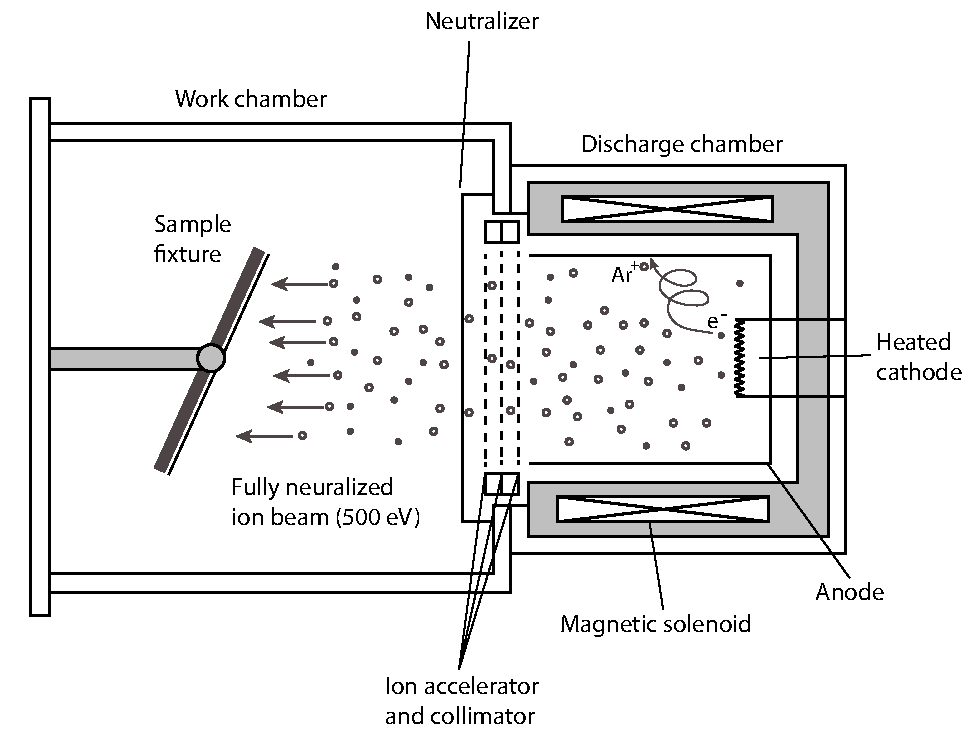
\includegraphics[width=1.0\textwidth]{Drawing/IonMill.pdf}
	\caption[Simplified view of ion mill]{Simplified view of ion mill. The argon ions are generated from the discharge chamber on the right-hand side. Electrons are extracted from the heated cathode and ionize Ar molecules. A magnetic field is applied through a solenoid to increase electrons' path. Ar$^{+}$ are accelerated to a kinetic energy of 500 eV and aligned by the grids. Electrons from the neutralizer are mixed with the Ar$^{+}$ plasma flow so that the collimation is maintained. The sample is tiled by an angle of 22.5$^{\circ}$ from normal.}
	\label{FIG:IonMill}
\end{figure}

\subsection{Deposition}

Titanium and gold are used for making contact with the interface of LAO/STO. In this research, two methods are used to deposit metals: sputtering and electron-beam (e-beam) evaporation. Sputtering is similar to ion milling, but instead of using Ar$^{+}$ plasma flow to bombard and etch the sample, it is directed towards the target materials (Ti, Au, etc.). The binding energy of the target material atoms is much smaller than the kinetic energy of Ar$^{+}$; materials are ejected from the target and deposit onto the sample surface. E-beam evaporation (Figure \ref{FIG:Ebeam}) controls electron-beam to heat the target material and vaporize it. The vapor travels through a long distance ($> 10$ cm) before it reaches the sample. Compared to sputtering, the e-beam evaporation is more directional.

\begin{figure}[p]
	\centering
	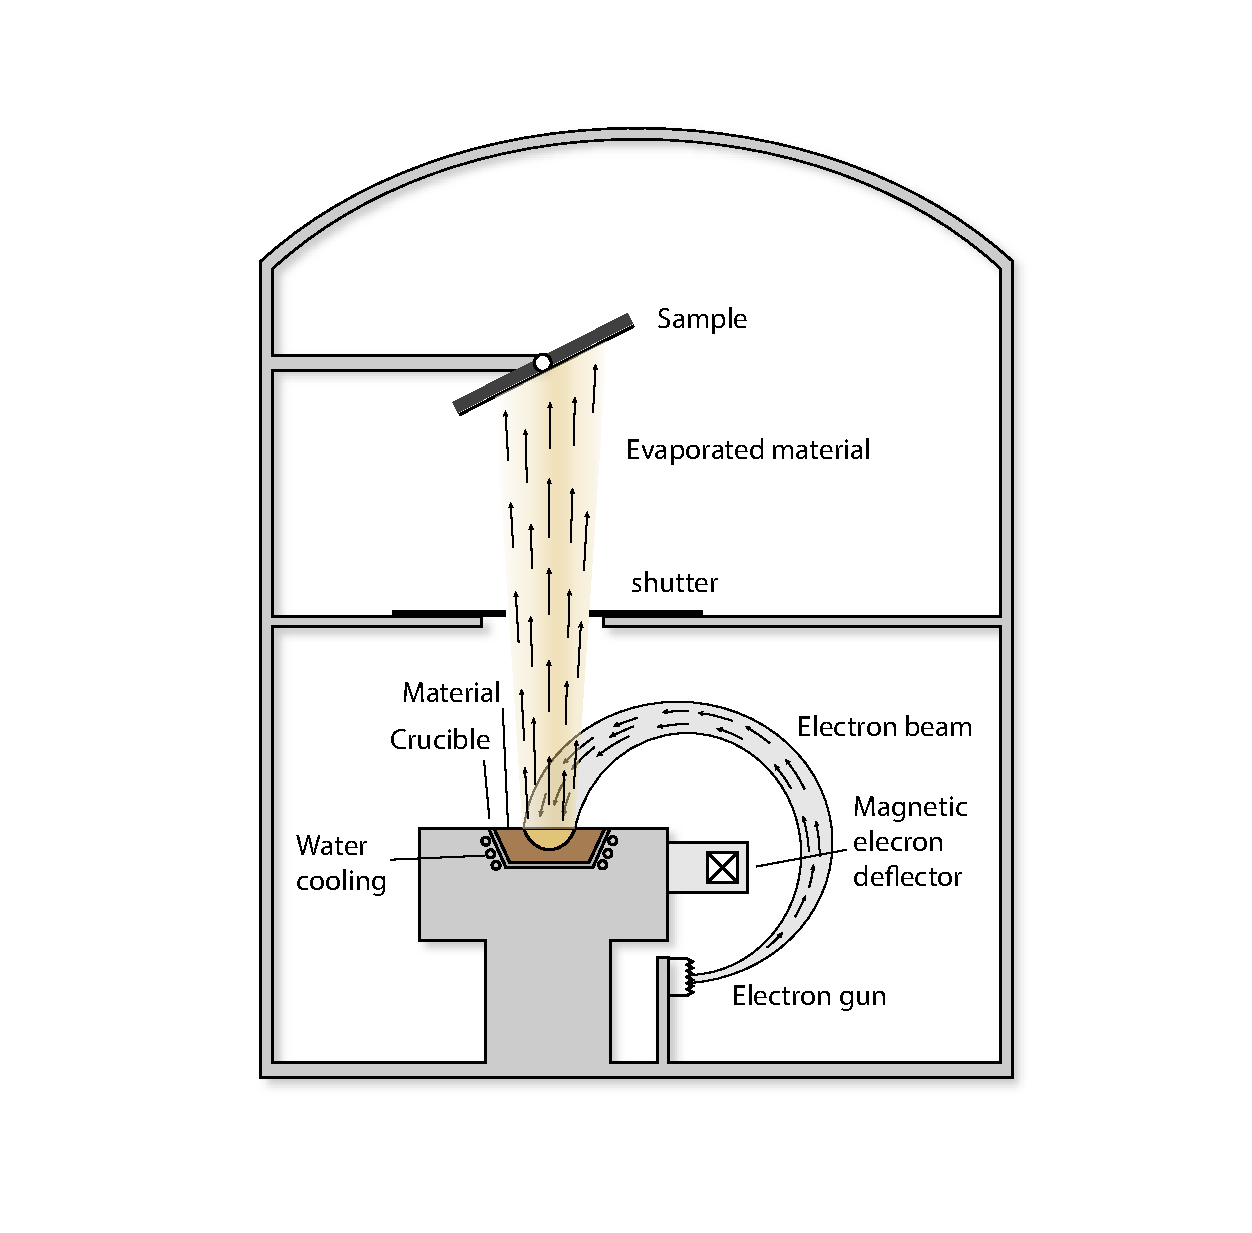
\includegraphics[width=1.0\textwidth]{Drawing/Ebeam.pdf}
	\caption[E-beam evaporator]{E-beam evaporator. The electron beam is generated from an electron gun on the bottom. The beam is deviated and shaped by the magnetic field, towards the material. The material is loaded in a crucible and heated up to the melting point. The vapor of the material is thrown towards the sample on top. A shutter controls deposition time.}
	\label{FIG:Ebeam}
\end{figure}

As shown in Figure \ref{FIG:Ebeam}, a beam of electron is accelerated by a high voltage ($\sim$ 10 kV). The direction and shape of the beam are controlled by magnetic field. The material is loaded in a crucible and heated up by the e-beam and evaporated. The material is thrown upward, to the loading chamber where the sample is located. A shutter is used to control the deposition time of the material. The e-beam current controls the deposition rate. The sample can be tilted to improve the electrical contact to the interface. The pressure of the chamber is maintained at $< 10^{-6}$ Torr to avoid oxidation of material during deposition. Also, when titanium is used to make contact between gold bonding pads and LAO/STO interface, a pre-deposition evaporation of 10 minutes is performed. The evaporated titanium can trap the remaining oxygen molecules in the chamber, and further reduce the chamber pressure.

\subsection{Lift-off}

When the sample is patterned with photolithography and coated with metal, the photoresist and the excessive metal need to be removed. The photoresist can dissolve in organic solvents such as acetone. Then the sample is washed with IPA to remove the acetone residue. 1165 remover (1-methyl-2-pyrrolidone, or NMP) need to be used for lift-off if the has been heated up to 140 $^{\circ}$C and cross-linked.

\subsection{Oxygen plasma cleaning}

The oxygen plasma cleaner activates oxygen molecules with a high-frequency voltage (kHz to MHz) in low pressure and forms plasma or oxygen radicals when electrons recombine with oxygen ions. The mixture is highly reactive with organic materials like photoresist residue. Oxygen plasma cleaning can be categorized as a form of RIE, but it usually operates at the high end of 100 mTorr, and the etching is less directional. Compared to chemical solvent, oxygen plasma removes the photoresist residue at a much lower speed (about 10 nm/min) but does less damage to the LAO/STO interface compared to RIE. Therefore, oxygen plasma cleaning is used as the final step for sample processing.

\section{Atomic force microscope}
\label{SEC:AFM}

The atomic force microscope (AFM) is a type of instrument that uses a nanoscale probe to interact with the surface, and characterize the properties (topography, electric potential, conductivity, etc.). It was invented in IBM Lab by Binning \textit{et al.} \cite{binning1986atomic} in 1986. The development of AFM technology benefited from the advancement of STM and precise closed-loop spatial control using the piezoelectric effect. AFM was invented to overcome the drawback of STM --- only conductive or semi-conductive samples can be measured. It can measure various types of interaction between the probe and surface, such as surface potential, magnetic force, van de Waals force, etc. Also, unlike the scanning electron microscopy (SEM) or tunneling electron microscopy (TEM), the AFM can be operated in various environment (aqueous, ambient, vacuum or cryogenic), and does not require the sample to be pre-treated (such as metal coating) or being conductive. The robustness and non-invasive nature of AFM make it a powerful tool for studying surface phenomena including 2D charge density, magnetic dipole moment, capacitance, chemical bonding, and nano-device lithography. AFM can also be integrated with other techniques, such as infrared spectroscopy\cite{hammiche1999photothermal, pollock2006handbook}. The limitation of AFM is that the imaging cannot be as fast as SEM or TEM, as it relies on the physical movement of the tip.

\subsection{Working principle}

The AFM mainly consists of three parts, as shown in Figure \ref{FIG:AFM}, AFM tip, laser optics, and piezoelectric scanning system. The AFM tip has a sharp end, with a radius of curvature in the nanometer scale. A laser is reflected from the top surface the AFM tip and collected by a quad detector. The quad detector determines the position by
\begin{equation}
\begin{split}
I_\mathrm{sum} & = I_A + I_B + I_C + I_D \\ 
I_\mathrm{vdiff} & = (I_A + I_B) - (I_C + I_D) \\ 
I_\mathrm{hdiff} & = (I_A + I_C) - (I_B + I_D),
\end{split}
\end{equation}
where $I_A$, $I_B$, $I_C$, and $I_D$ are the intensities on the four quadrants of the detector. $I_\mathrm{sum}$ is the total intensity. $I_\mathrm{hdiff}$ and $I_\mathrm{vdiff}$ are the horizontal difference and vertical intensity difference. Assume the laser spot has Gaussian distribution. When the center of laser spot changes, the distribution of intensity on the four quadrants would change. The detector can monitor the movement by the horizontal and vertical differences in intensities. 

\begin{figure}[h!]
	\centering
	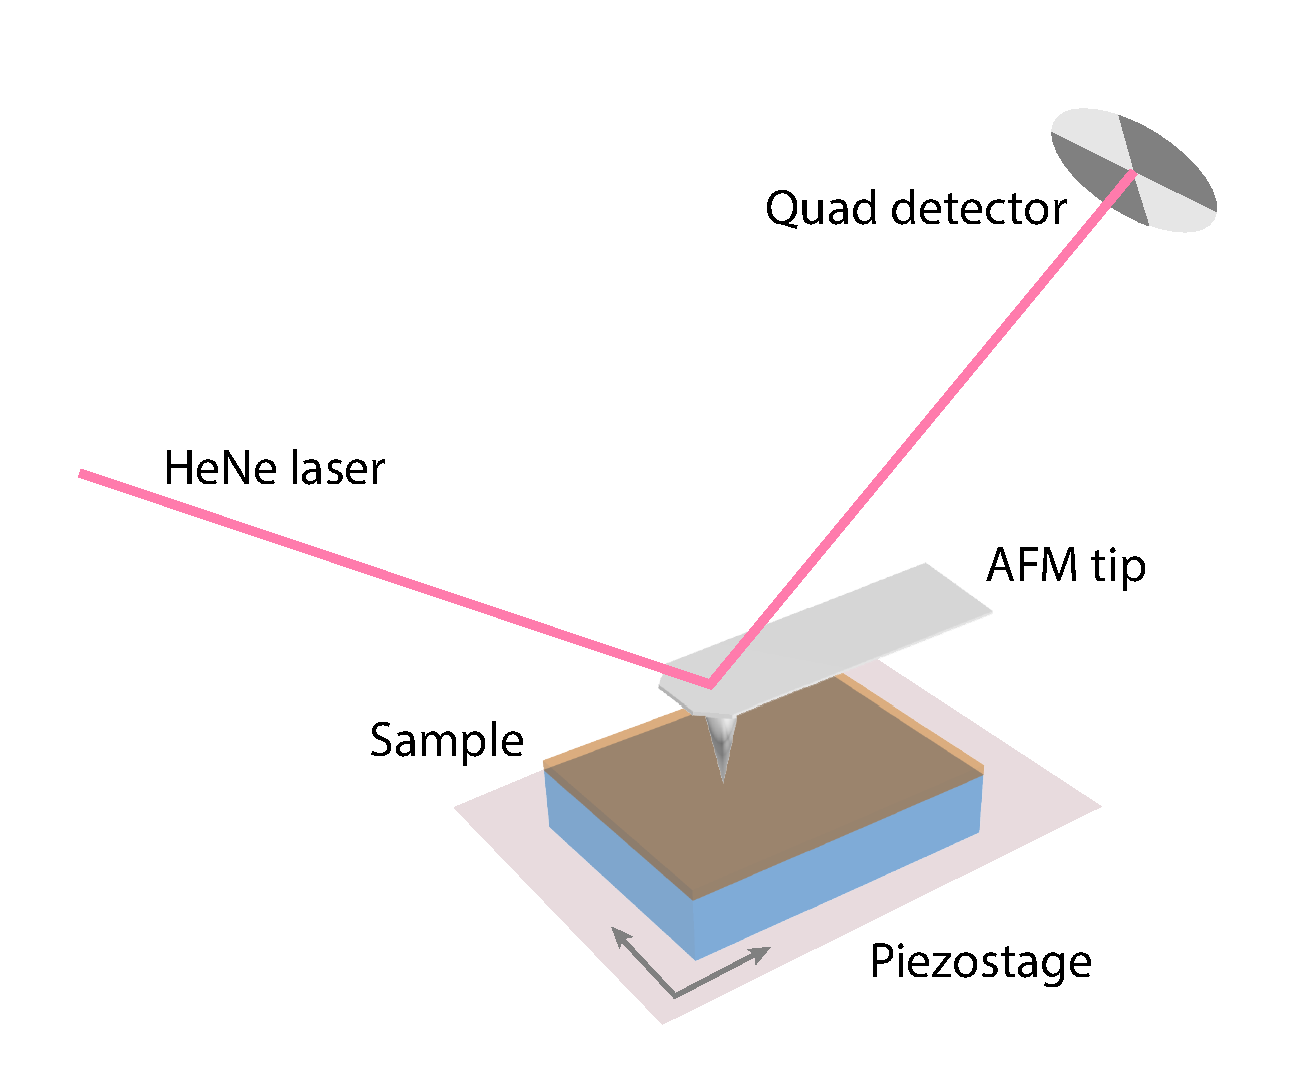
\includegraphics[width=0.7\textwidth]{Drawing/AFM.pdf}
	\caption[The schematics of AFM]{The schematics of AFM. A laser is reflected from the top surface of the AFM tip, and collected by a quad detector. A small amount of deformation would cause the center of laser spot to move on the quad detector, and measured as a change of differential voltage.}
	\label{FIG:AFM}
\end{figure}

When the interaction between the tip and sample surface changes and the tip is slightly deformed, the laser spot will move on the quad detector. The deformation of tip follows Hooke's law:
$$F = -k \cdot x$$
Where $x$ is the amount deformation, and $k$ is the spring constant of the tip's cantilever. $k$ is mostly between 0.1 N/m and 100 N/m, depends on the type of the tip. In this research, tips with spring constant $k = 3$ N/m are used. The interaction between the AFM tip and the sample surface is a function of distance. The attractive interaction decays slower than the repulsive interaction. Therefore the total interaction follows the curve in Figure \ref{FIG:Interaction}.

\begin{figure}[h!]
	\centering
	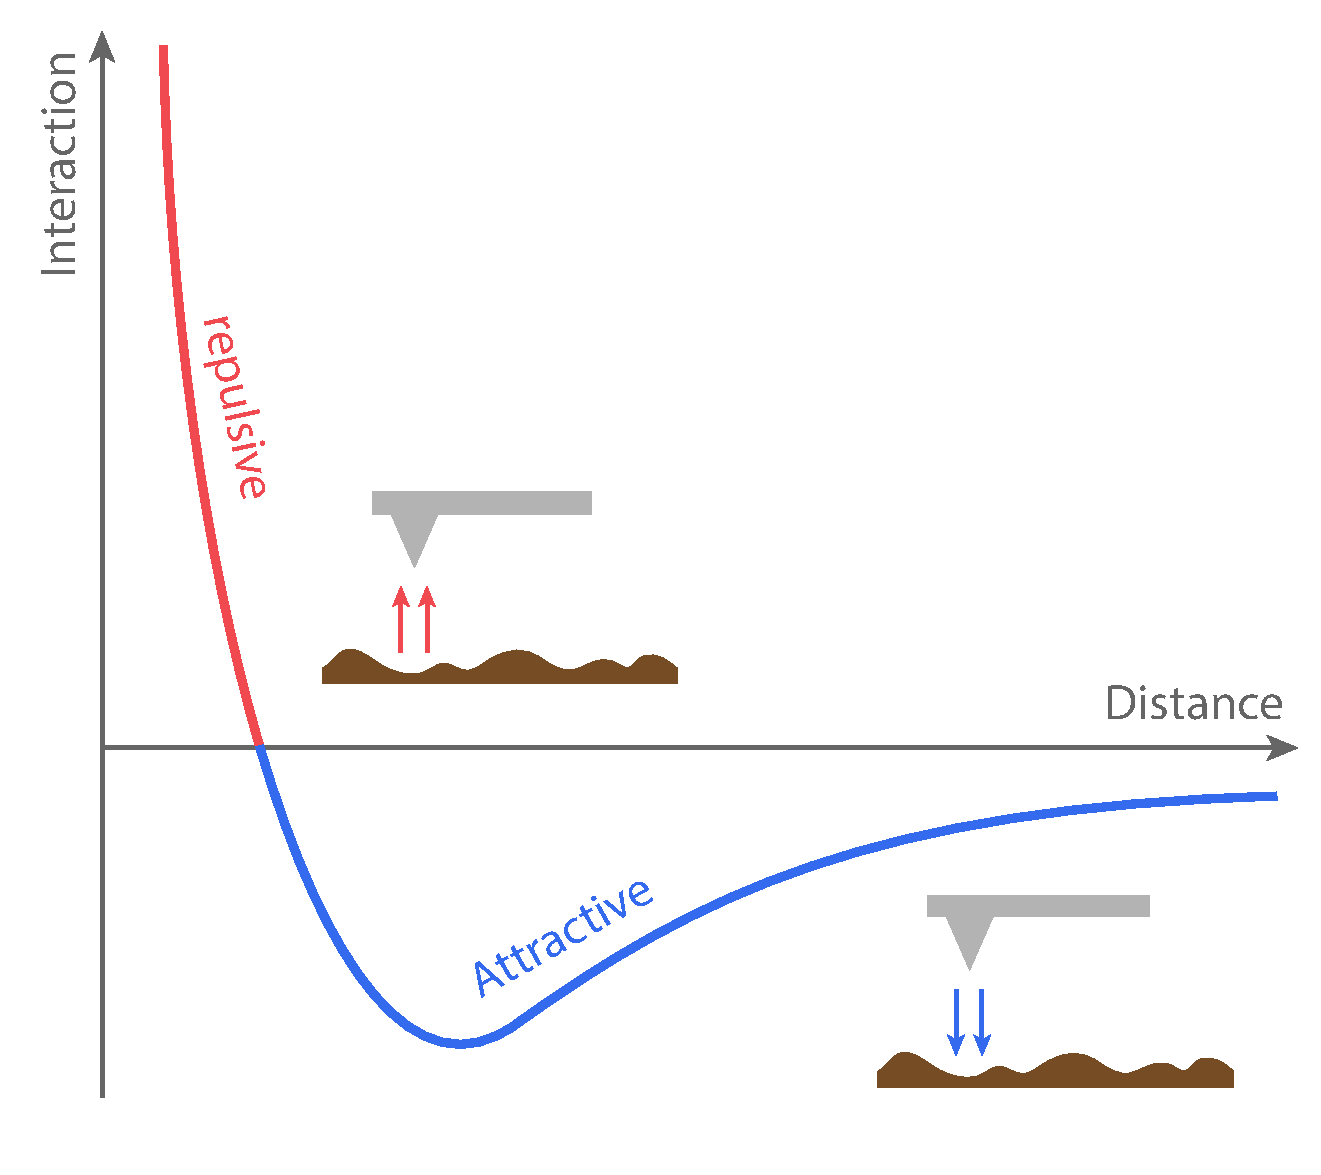
\includegraphics[width=0.6\textwidth]{Drawing/Interaction.pdf}
	\caption[The interaction between the tip and the sample surface]{The interaction between the tip and the sample surface. In the long distance the interaction zero. When the tip moves towards the sample, the interaction is attractive. As the tip gets closer, the interaction would switch from attraction to repulsion.}
	\label{FIG:Interaction}
\end{figure}

The sample is located on the piezoelectric scanning stage. The movement of the sample and the tip and the signal from the laser optics system are controlled and monitored by a computer. The type of signal depends on the working mode of AFM and nature of the interaction. More details are discussed in the following sections. 

\subsection{Contact mode}

In contact mode, the AFM tip is in close contact with the sample and the interaction is repulsive. A piezoelectric actuator controls the distance between the tip and the sample. As shown in Figure \ref{FIG:ContactAFM}, When the tip approaches the sample surface, repulsion from the sample would deform the tip and changes the reflection angle of the laser spot. The intensity difference on the quad detector would also change, in terms of a voltage signal. When the sample is driven by the piezostage and the tip moves relative to the sample, the repulsive force between the tip and sample surface is regulated by a feedback loop between deflection voltage and the piezoelectric actuator so that the tip deformation and force are constant. 

\begin{figure}[h!]
	\centering
	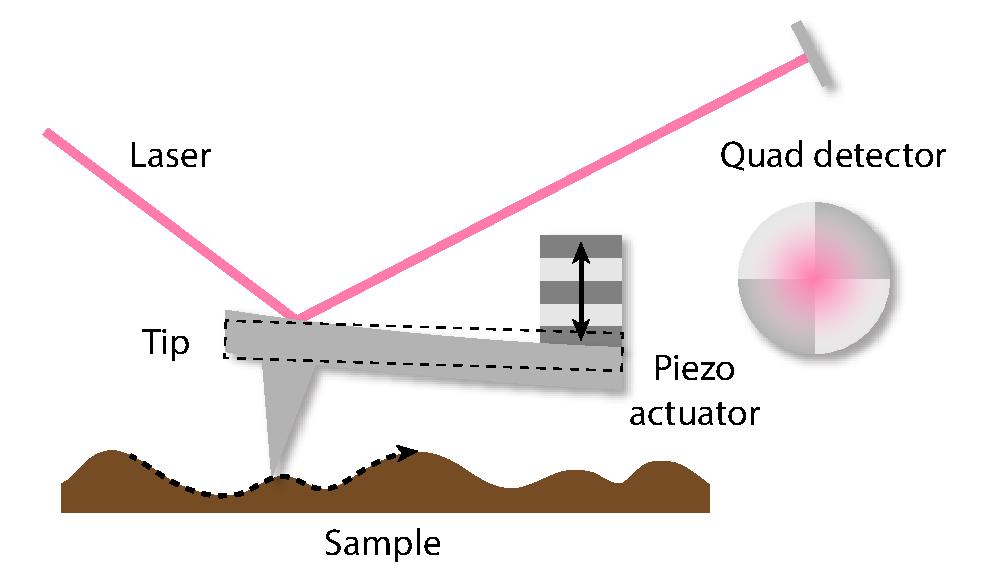
\includegraphics[width=0.6\textwidth]{Drawing/ContactAFM.pdf}
	\caption[AFM contact mode]{AFM contact mode. The tip is pressed to the sample surface by the piezoelectric actuator. The quad detector monitors the deformation of the tip.}
	\label{FIG:ContactAFM}
\end{figure}


\subsection{AC mode}

In AC mode, the AFM tip is driven by a sinusoidal electrical signal on the tip piezoelectric actuator, as shown in Figure \ref{FIG:ACAFM}. The electric frequency is close to the resonance frequency of the tip (10 kHz -- 500 kHz). The driving frequency is not set exactly at the resonance frequency so that the gradient of amplitude change is maximized and the system is most sensitive to the interaction change. When the tip approaches the sample surface, the interaction between the tip and surface will cause the resonance frequency to shift, and changes the amplitude $A$ and phase $\theta$ of the tip oscillation. When the tip scan through the surface, $A$ and $\theta$ are recorded for each position on the sample surface and mapped onto a 2D image. A feedback loop controls the voltage on the piezoelectric actuator ($z$ voltage) so that the amplitude $A$ is maintained at the set point.

\begin{figure}[h!]
	\centering
	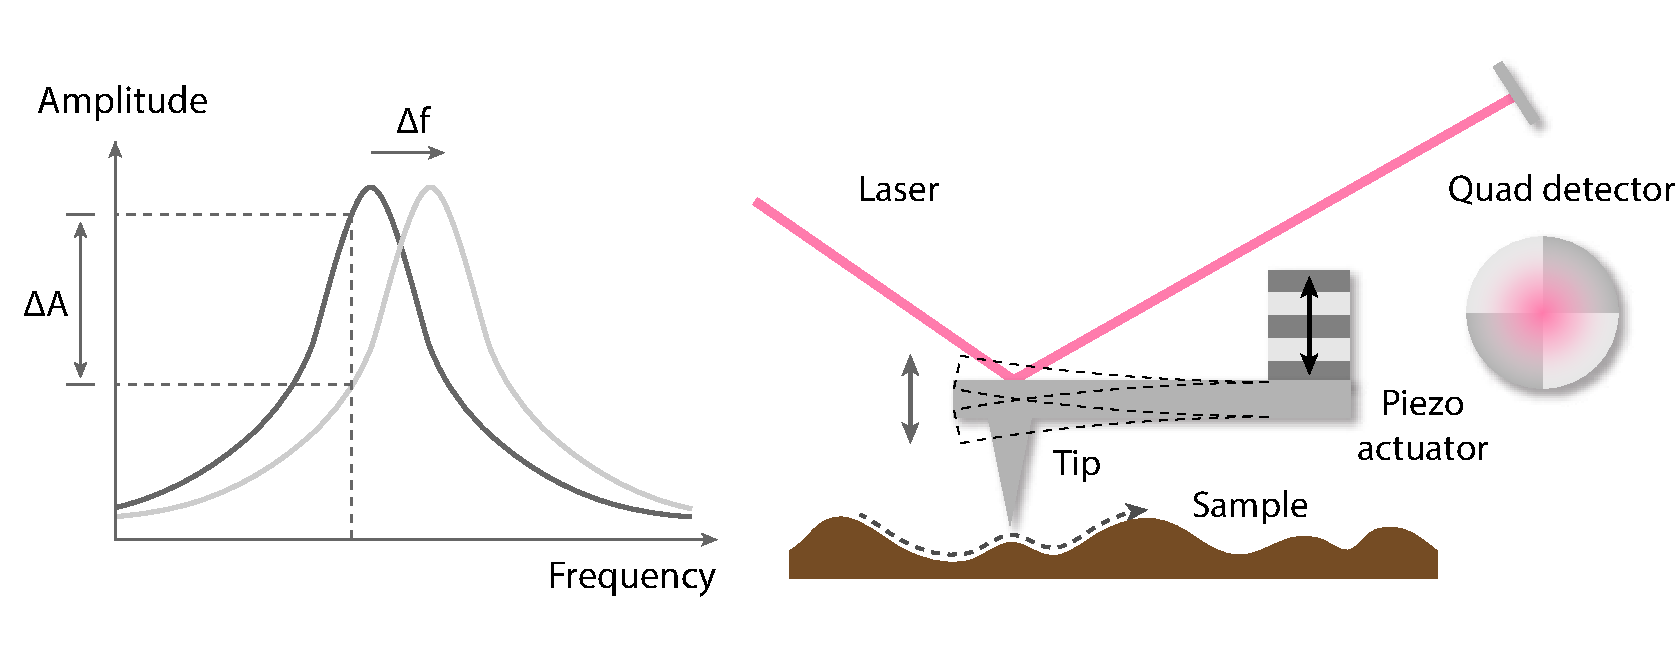
\includegraphics[width=1.0\textwidth]{Drawing/ACAFM.pdf}
	\caption[AFM AC mode]{AFM AC mode. Left: the tip is driven at a frequency close to the resonance frequency. When the resonance frequency shifts as the interaction between the tip and the sample changes, oscillation amplitude is monitored by the quad detector.}
	\label{FIG:ACAFM}
\end{figure}

\subsection{Non-contact mode}

In the non-contact mode, the tip is maintained at the attractive regime so that the sample does not have direct contact with the tip. The tip and the sample are kept at a distance that the interaction is always attractive while the tip is scanning through the sample (Figure \ref{FIG:NonContactAFM}). 

\begin{figure}[h!]
	\centering
	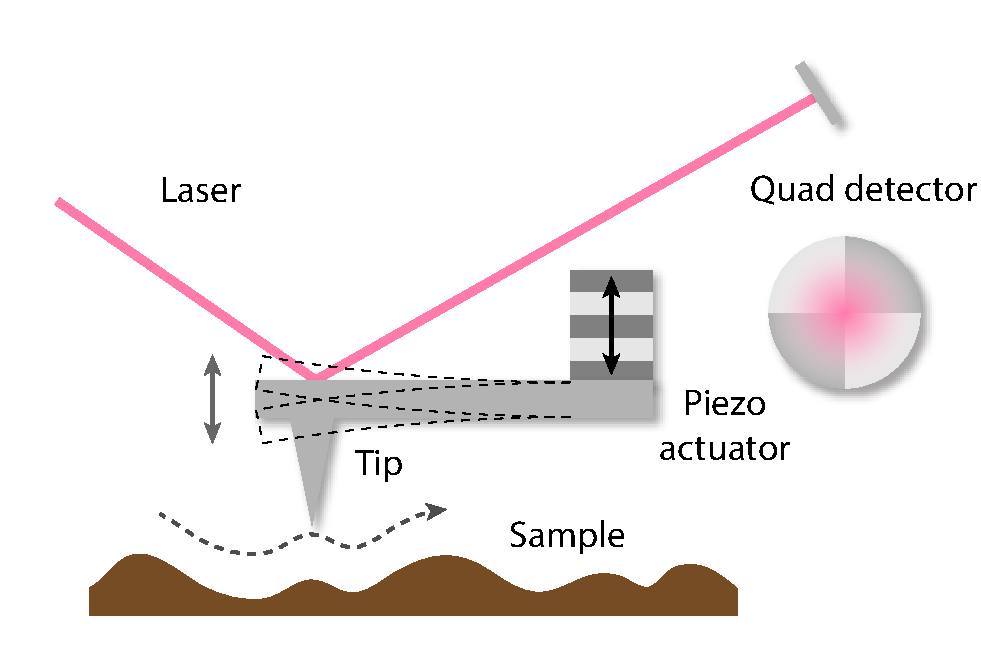
\includegraphics[width=0.6\textwidth]{Drawing/NonContactAFM.pdf}
	\caption[AFM Contact mode]{AFM Contact mode. The tip is kept at a distance from the sample so that the interaction is always attractive. The tip does not have direct contact with the sample during the scanning.}
	\label{FIG:NonContactAFM}
\end{figure}

\subsection{Magnetic force microscopy}
\label{SEC:AFMMFM}

When the tip is coated with ferromagnetic materials (e.g., Co, Fe), the AFM can measure the magnetic interaction with magnetic force microscopy (MFM). Similar to AC mode, the tip is driven by an oscillating AC voltage close to the resonance frequency and the change of interaction is monitored by the amplitude $A$ and phase $\theta$ of the differential voltage from the quad detector. The challenge of MFM is that the magnetic and van der Waals interactions are coupled together. The two-pass technique is used to solve this problem. In the first scan, the tip scans the sample close to the surface and measures the topography. In the second scan, the tip is lifted and maintained at a constant distance (such as 50 nm) from the sample surface using the height information obtained from the previous scan, so that the van der Waals interaction is negligible, and the spatial gradient of magnetic force can be measured\cite{hartmann1999magnetic}:
\begin{equation}
%\begin{split}
\label{EQN:MFM}
\Delta A \approx \frac{2 A_0 Q}{3\sqrt{3k}} \cdot \frac{\partial F_z}{\partial z}, \ \ \ \
\Delta \phi \approx \frac{Q}{k} \cdot \frac{\partial F_z}{\partial z}, \ \ \ \
\Delta f \approx -\frac{f_0}{2k} \cdot \frac{\partial F_z}{\partial z}, 
%\end{split}
\end{equation}
where $\Delta A$, $\Delta \phi$ and $\Delta f$ are the change of amplitude, phase and resonance frequency; $A_0$ and $f_0$ are the original amplitude and frequency; $Q$ and k are the resonance quality factor and cantilever spring constant. $\partial F_z/\partial z$ is the spatial gradient of magnetic force. 

Like contact and AC mode of AFM, the resolution of MFM is limited by the tip radius of curvature. Ferromagnetic coating of the MFM tip is about 40 nm in this research and the resolution is in the same order of magnitude. 

The advantage of MFM is that the resolution and sensitivity are higher than other methods such as magneto-optical effect imaging. The downside of MFM is that the imaging speed is limited by the raster scanning speed. The two-pass method takes twice as long as usual AFM AC scanning. Also, as equation (\ref{EQN:MFM}) shows, MFM signal is not determined by the absolute value of magnetic force but is proportional to the spatial gradient of the force $\partial F_z/\partial z$. Therefore the scanning speed would also affect the signal. AFM tip can also affect the magnetic dipoles in the sample, and the MFM image would change after each scan. Other long-range interaction such as Coulomb interaction cannot be eliminated by the two-pass method. In spite of these disadvantages, the MFM is still a powerful tool to study surface magnetism for its high sensitivity.

\begin{figure}[h!]
	\centering
	\vspace{0.85cm}
	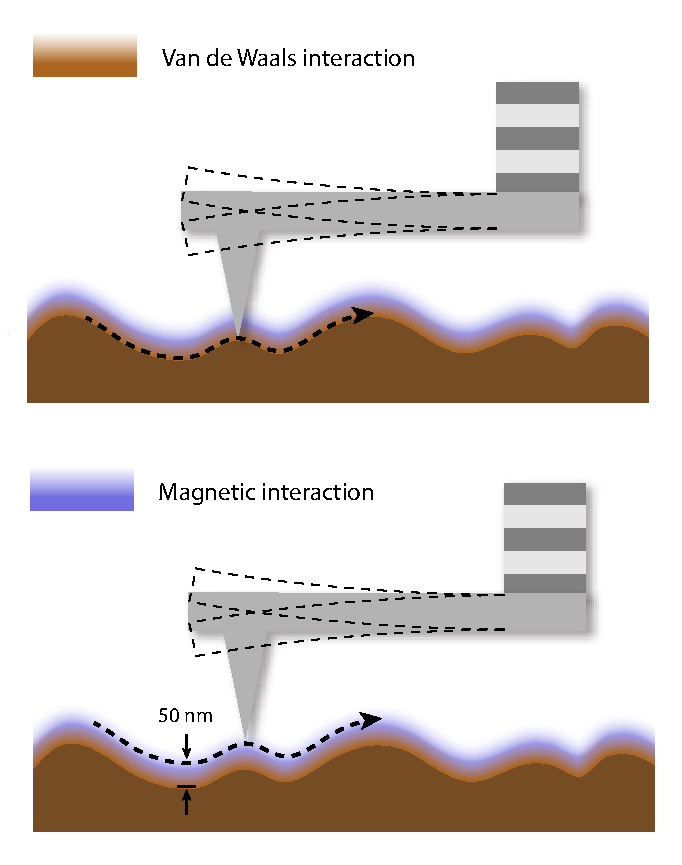
\includegraphics[width=0.5\textwidth]{Drawing/MFM.pdf}
	\caption[MFM mode]{MFM mode. The first scan is close to the sample surface so that the topographical information can be obtained. In the second scan the tip is lifted to a constant distance from the sample surface so that the long-ranged magnetic interaction can be decoupled from topography signal.}
	\label{FIG:MFM}
\end{figure}

\subsection{Piezoresponse force microscopy}

The high sensitivity and extendability of AFM make it a versatile tool to measure different types of interactions between the tip and sample. One important variant is piezoresonse force microscopy (PFM). When an external stress or strain is applied to a piezoelectric material, the deformation will induce electric dipole moments and build up an internal electric potential across the sample. Inversely, the external electric field can also induce mechanical deformation. Depending on the properties of the material, the deformation can be either expansion or contraction. The effect can be described with
$$
X_i = d_{ki}E_k,
$$
where $X_i$ is the strain tensor, $d_{ki}$ is the piezoelectric tensor and $E_k$ is the electric field. For a tetragonal system, 
$$
\begin{bmatrix}
X_{1} \\
X_{2} \\
X_{3} \\
X_{4} \\
X_{5} \\
X_{6}
\end{bmatrix} =
\begin{bmatrix}
0 & 0 & d_{31} \\
0 & 0 & d_{32} \\
0 & 0 & d_{33} \\
0 & d_{15} & 0 \\
d_{15} & 0 & 0 \\
0 & 0 & 0
\end{bmatrix}
\begin{bmatrix}
E_{1} \\
E_{2} \\
E_{3}
\end{bmatrix}
$$
When a field is applied in $E_3$ direction, the resulting non-zero strain terms are $X_1 = d_{31}E_3$, $X_2 = d_{32}E_3$ and $X_3 = d_{33}E_3$. Therefore, an electric field in the c-axis of the crystal will cause elongation in the c-axis and contraction in the other two orthogonal directions, or vice versa. The piezoresponse of sample can bring insights of the sample properties such as carrier concentration\cite{huang2013direct, guo2016correlations}, ferroelectric domain orientation\cite{soergel2011piezoresponse}, domain boundary\cite{potnis2011review}, etc. The piezoresponse of the LAO/STO system can be used to characterize the carrier density change on the interface.

\begin{figure}[p]
	\centering
	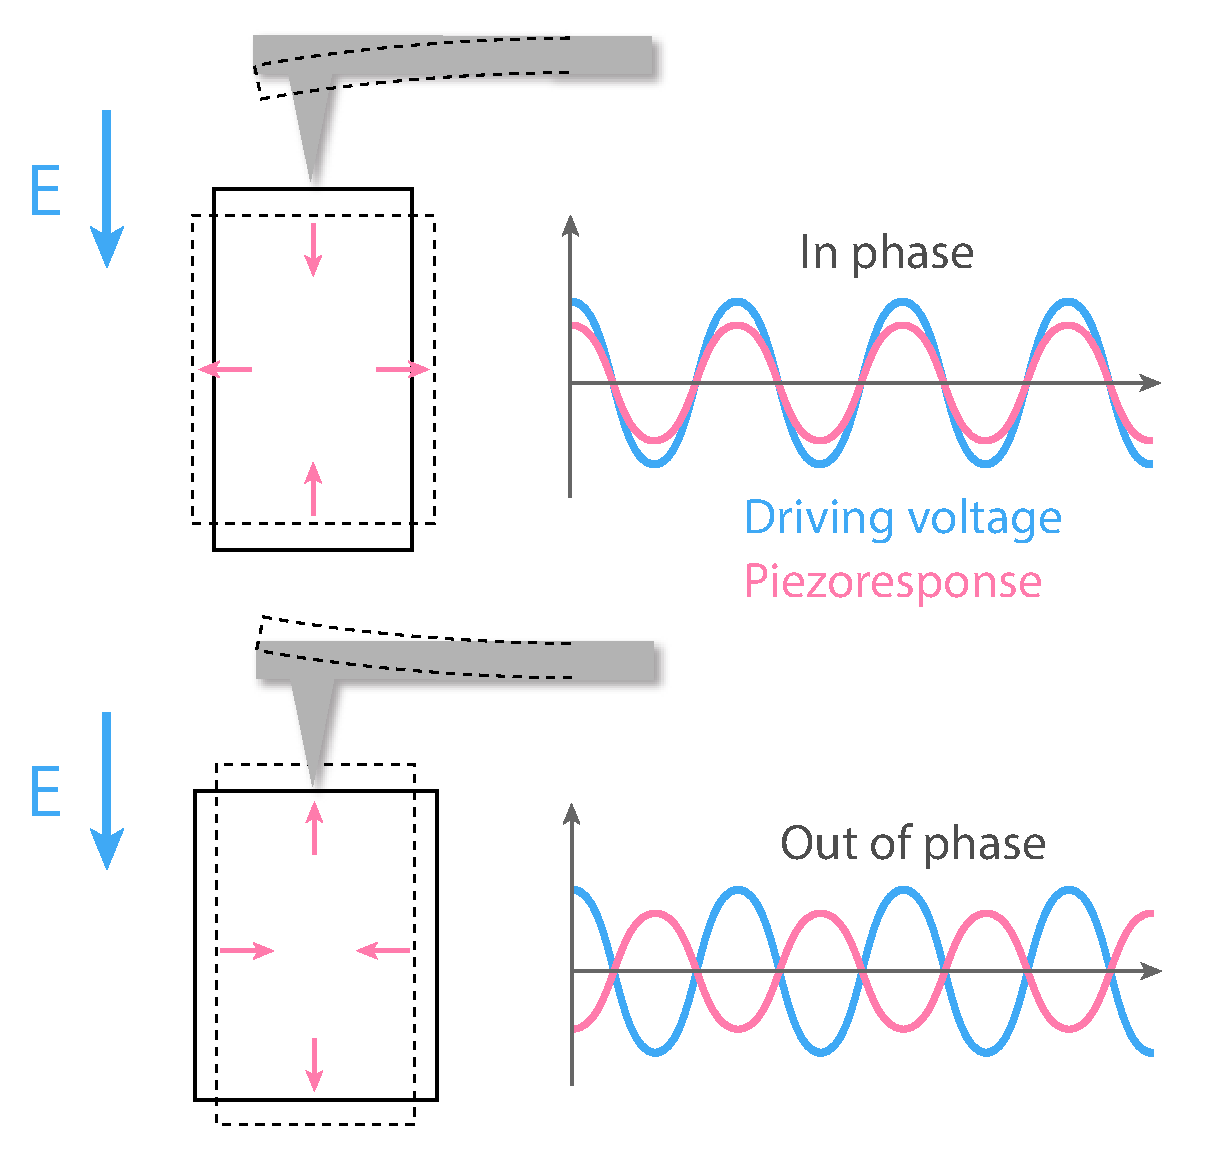
\includegraphics[width=0.7\textwidth]{Drawing/PFM.pdf}
	\caption[PFM mode]{PFM mode. The external electric field is applied to the sample surface through a conductive tip. The sample deforms and slightly bend the tip, and the deformation signal is monitored with a quad detector (not shown). If the sample contract in the direction of the field, the deformation signal is in phase with the driving voltage (above); if the sample elongate in the direction of the field, the signal would be out of phase with the driving voltage (below).}
	\label{FIG:PFM}
\end{figure}

In PFM measurement, a c-AFM tip is in contact with the sample, and a sinusoidal bias voltage is applied to the tip. For a sample with piezoresponse, the electric field will cause topography deformations. Since the sample is in contact with the tip, the topographical change of sample will induce slight changes of tip deformation. The sample deformation is usually in the order of 10 pm/V (e.g. $d_{33} = 85.6$ pm/V for BaTiO$_3$\cite{berlincourt1958elastic}). Therefore, the PFM signal is measured with the lock-in technique for the best signal-to-noise ratio. As shown in Figure \ref{FIG:PFM}, If the sample contracts in the direction of the electric field, the piezoresponse signal will be in phase with the electric signal; if the sample elongates in the direction of the field, the signal will be out of phase.

\subsection{LAO/STO nano-device c-AFM lithography}
\label{SEC:AFMLitho}

Other than performing surface characterization,one major application of c-AFM is to create nano-scale structures on the interface of LAO/STO. As discussed in Section \ref{SEC:WaterCycle}, the ``water-cycle'' mechanism\cite{bi2010water} and surface protonation\cite{brown2016giant} are central for the reversible AFM lithography on LAO/STO interface. The AFM is set in contact mode. When a positive voltage is applied to the conductive AFM tip, and $V_\mathrm{tip} > +6$ V\cite{cen2008nanoscale}, the electric field from the tip will dissociate the water molecules between the tip and sample surface, and leaves a trace of the proton, as the tip scans through the LAO surface. 

\begin{figure}[p]
	\centering
	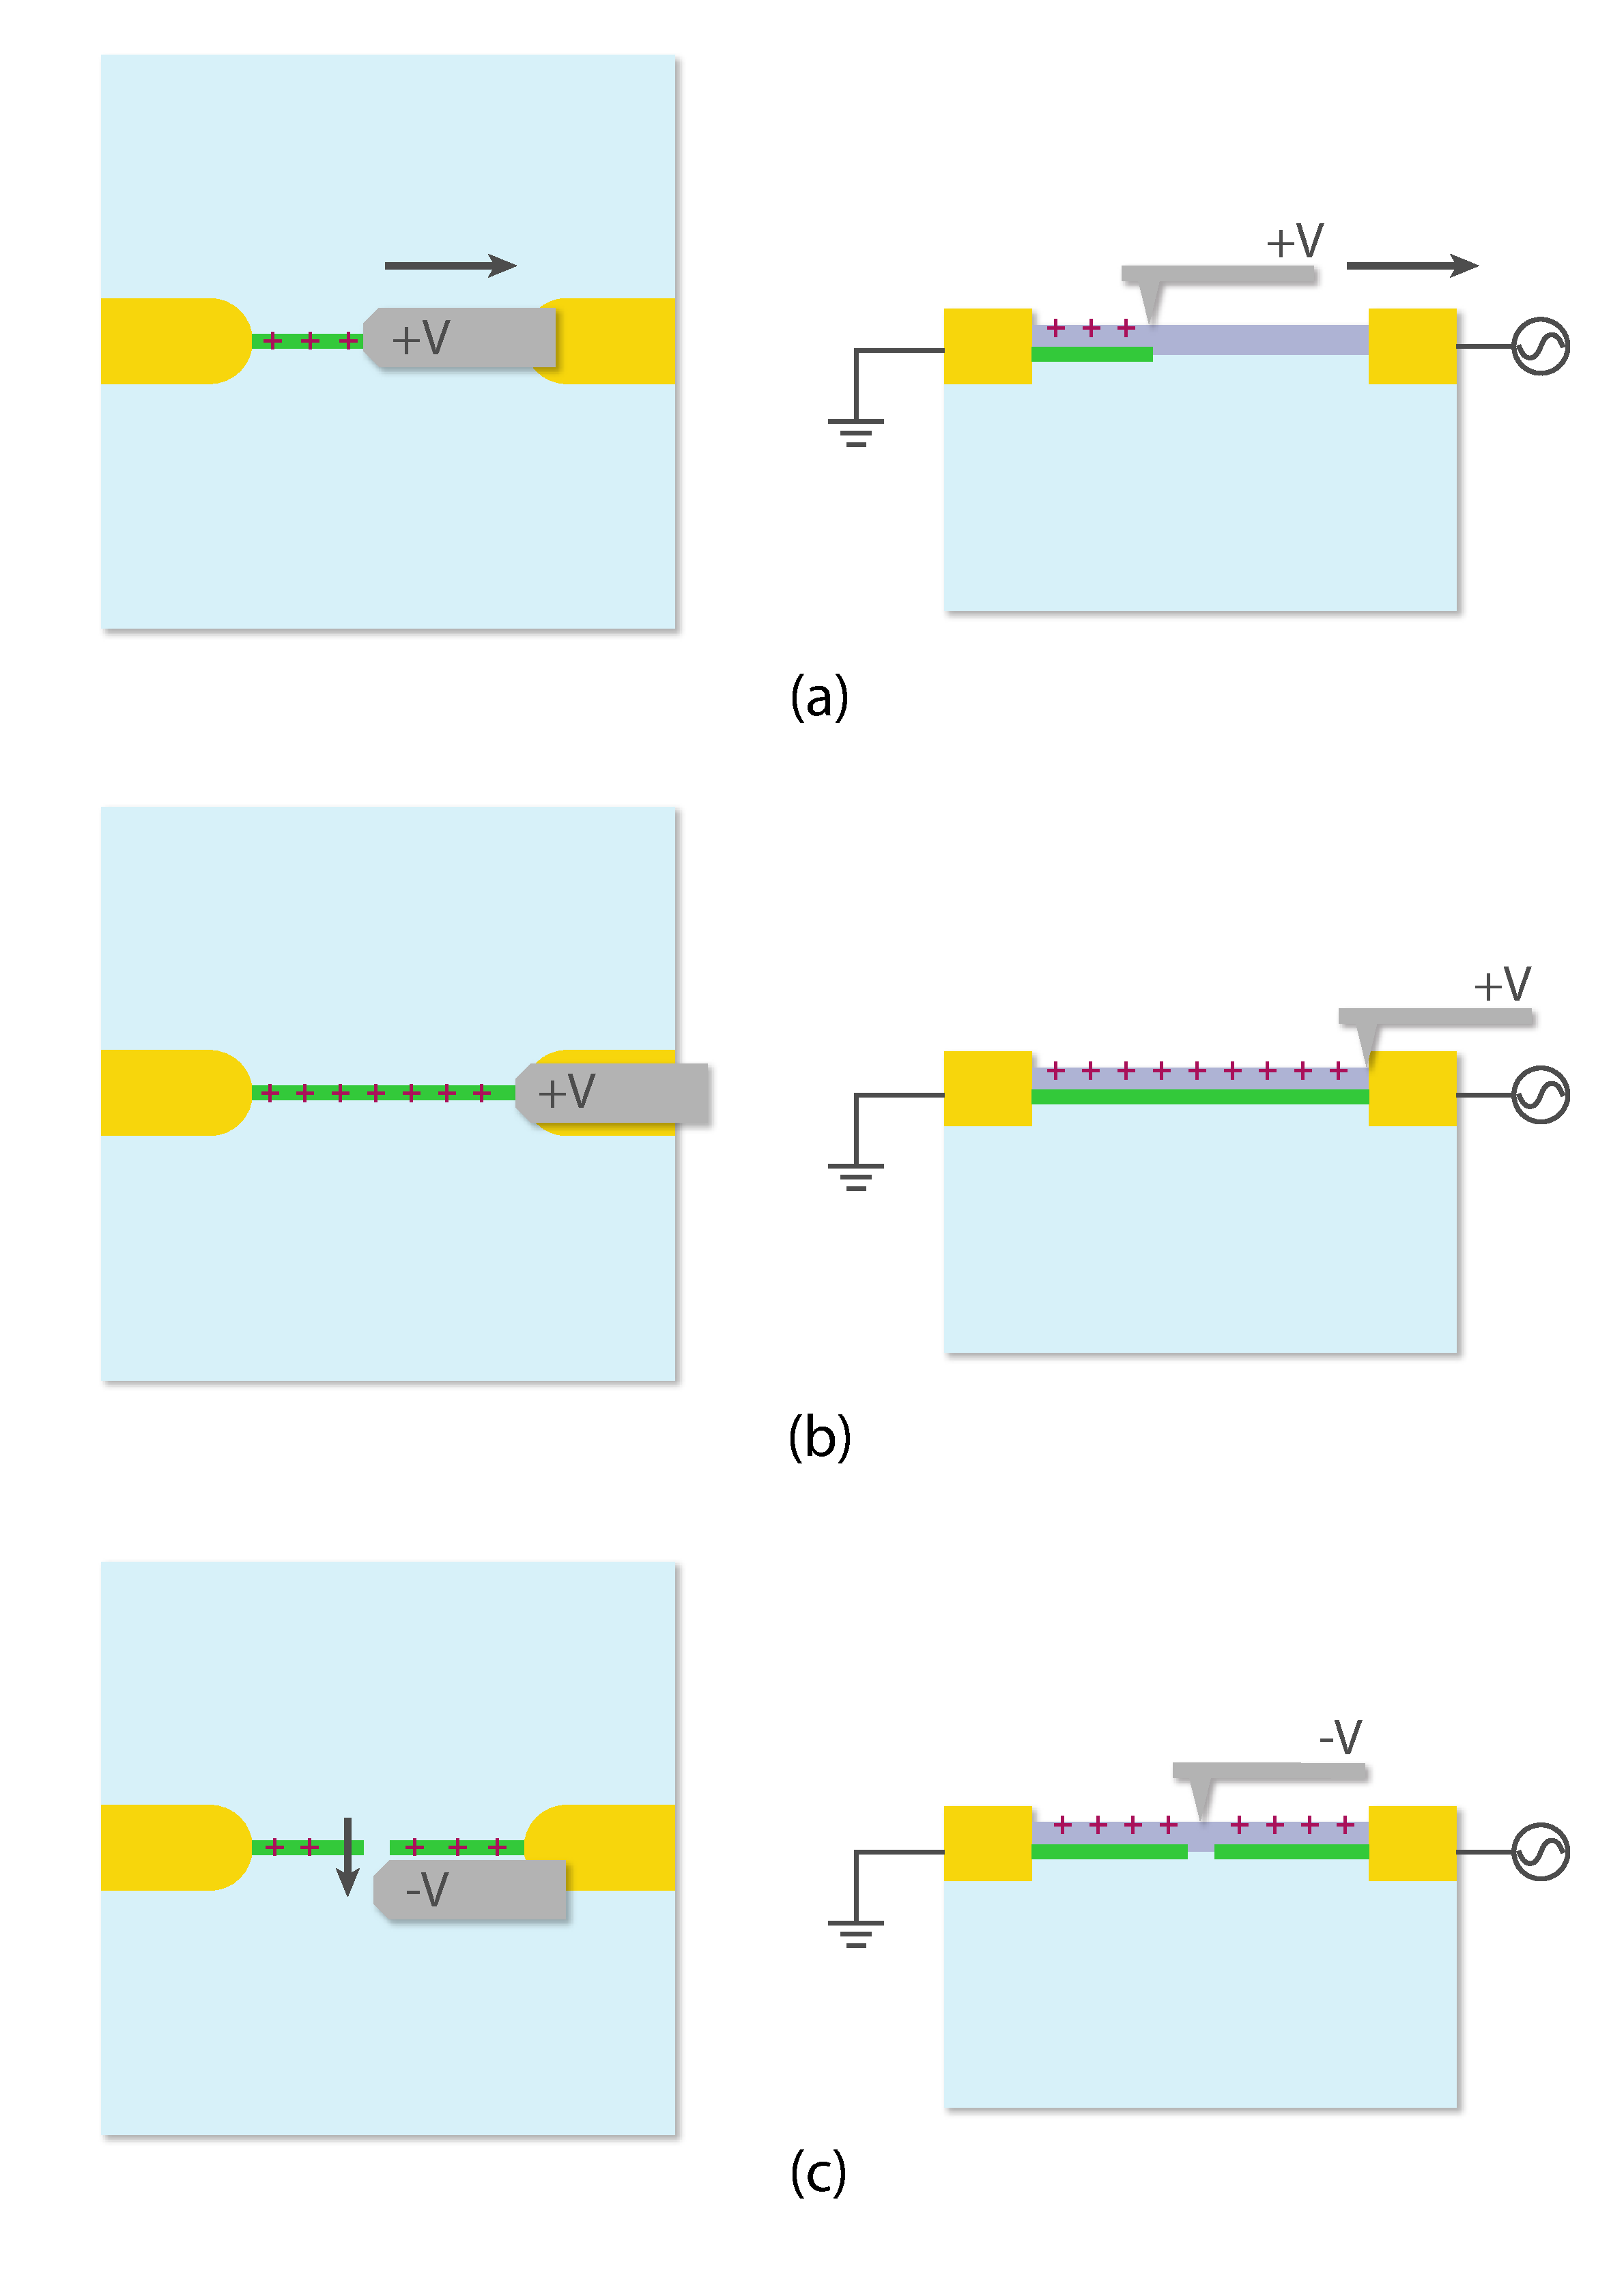
\includegraphics[width=.80\textwidth]{Drawing/Lithography.pdf}
	\caption[AFM lithography on LAO/STO]{AFM lithography on LAO/STO. (a)(b) The AFM is set in contact mode. A positive bias voltage is applied to the tip. A trace of the proton is left on the path of the AFM tip, and 2DEG is formed underneath the path. The conductivity between the two interface electrodes is monitored. (c) A negative voltage can remove the proton and create a gap on the nanowire.}
	\label{FIG:Lithography}
\end{figure}

As shown in Figure \ref{FIG:Lithography}, the golden regions are a pair of electrodes connected to the LAO/STO interface. An AC voltage of $\pm100$ mV is applied to one electrode, while the other electrode is connected to an ammeter for conductance measurement. Before the c-AFM lithography starts, the interface between the two electrodes is insulating. The current between them is monitored in real-time as the c-AFM tip scans through the surface. A positive voltage is applied, and protons are dissociated from the water meniscus and left behind the tip (plus signs in the Figure). 2DEG is formed under the protonated region and the interface becomes conductive (green area). Once the conductive channel connects the two electrodes, a current through the interface can be observed. When a negative voltage on the tip is applied, the protons will be removed from the surface and make the interface insulating again. Typical resistance of the nanowire is about 200 k$\Omega$/$\mu$m, and the width is in the same order of magnitude as the c-AFM tip\cite{cen2008nanoscale}. The nano-structure created by c-AFM can be imaged using PFM\cite{huang2015electric} or microwave impedance microscopy (MIM)\cite{jiang2017direct}. This technique can be applied to other oxide heterostructures as well\cite{li2014nanoscale, chen2018extreme}.

\begin{figure}[p]
	\centering
	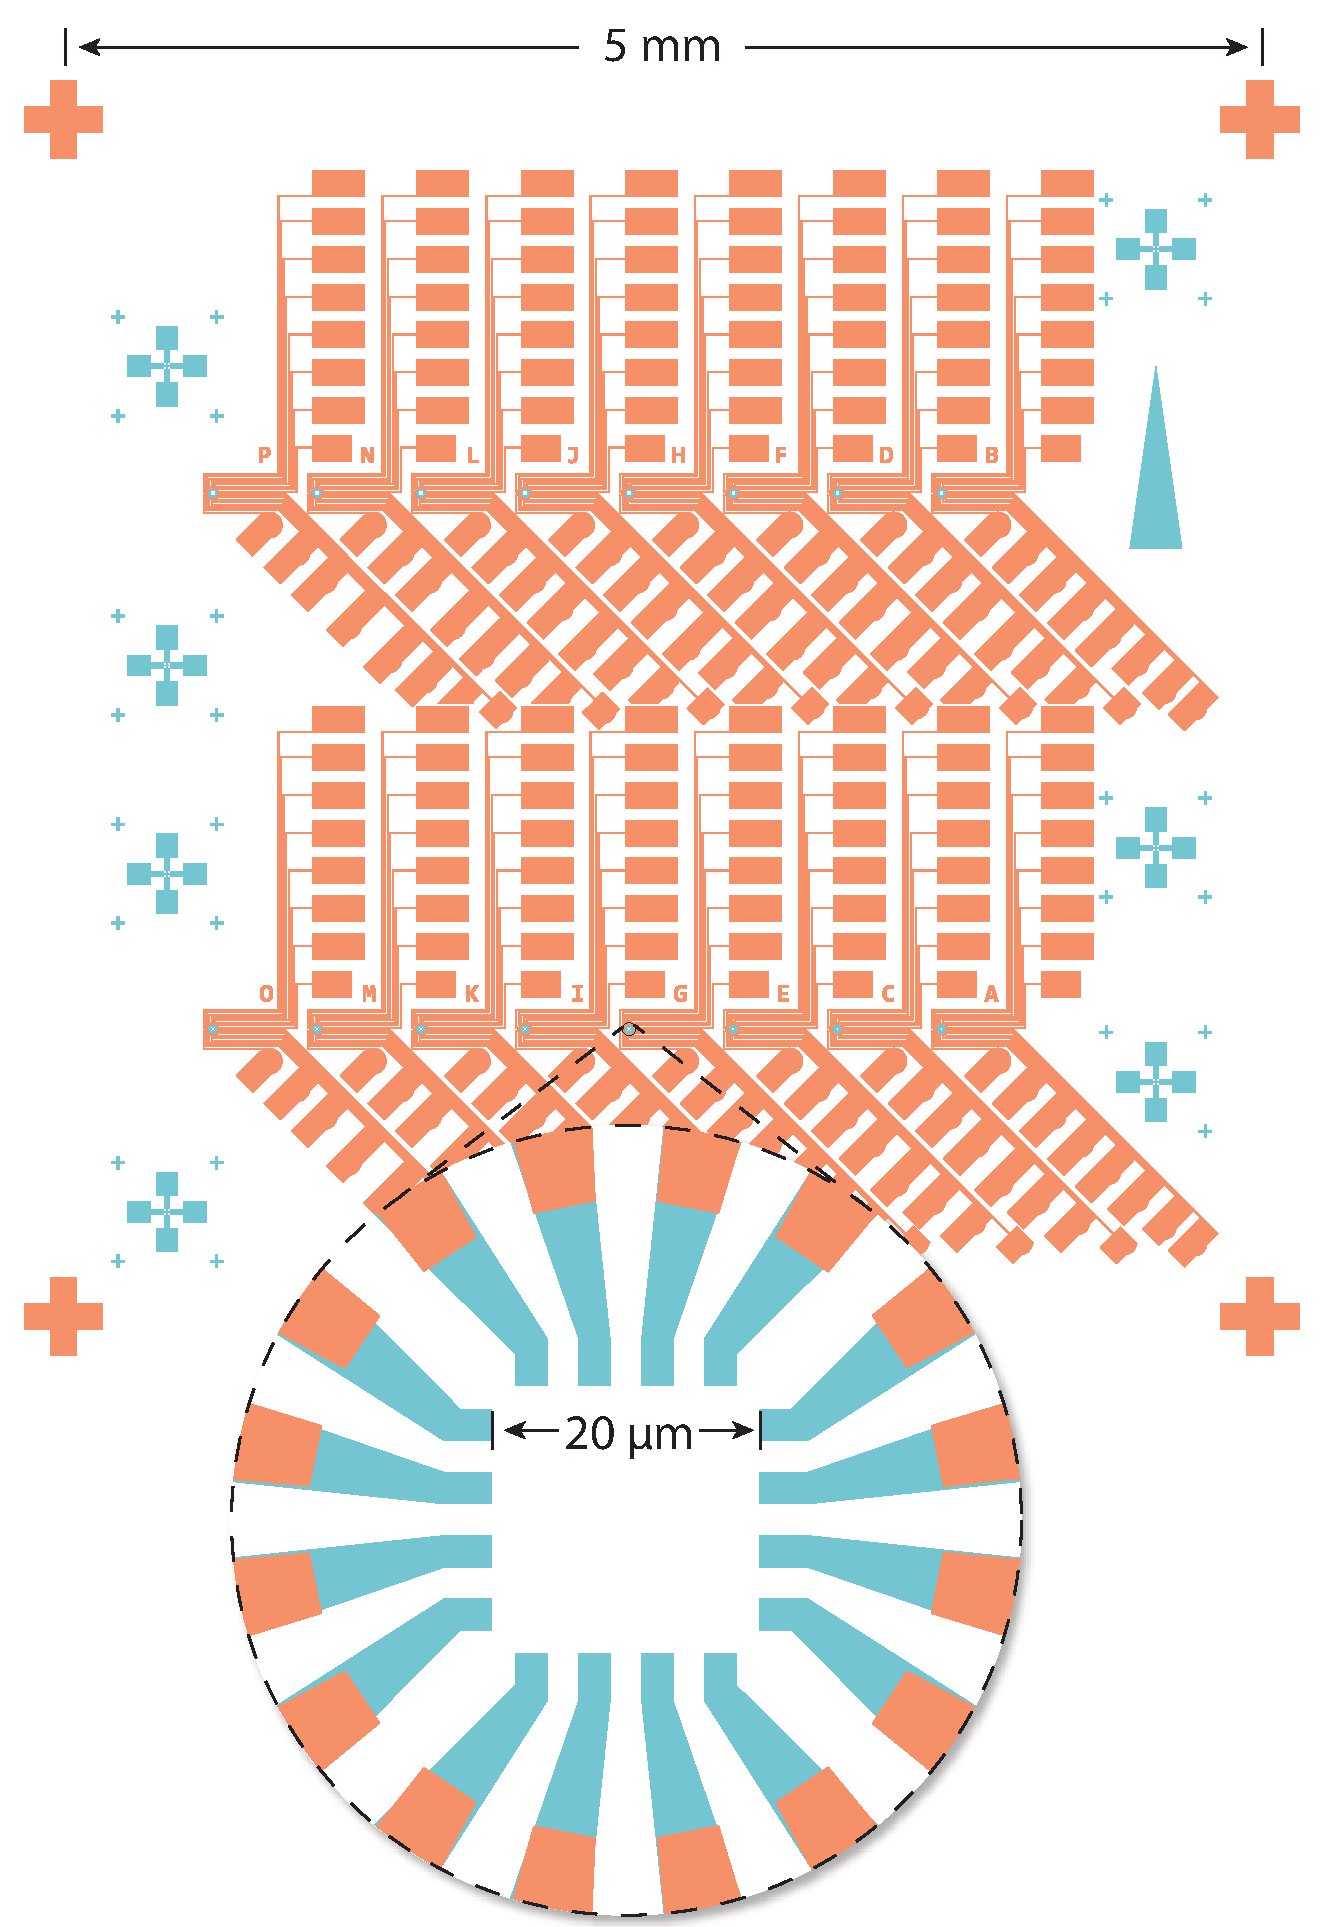
\includegraphics[width=1\textwidth]{Drawing/Regular.pdf}
	\caption[LAO/STO sample pattern for c-AFM lithography]{LAO/STO sample pattern for c-AFM lithography. The sample size is 5 mm $\times$ 5 mm $\times$ 1 mm. Canvas are 20 $\mu$m squares.}
	\label{FIG:Regular}
\end{figure}

The sample is patterned in such a way that and electrical measurement can be performed \textit{in situ} over the c-AFM writing. Figure \ref{FIG:Regular} shows the pattern of a typical LAO/STO sample for c-AFM lithography. The dimension of the sample is 5 mm $\times$ 5 mm $\times$ 1 mm. There are two layers of metals, where the blue layer is in direct contact with the LAO/STO interface. The sample is first etched with Ar ion mill, and the etched areas are backfilled with 4 nm of Ti and 25 nm of Au (as discussed in section \ref{SEC:IonMilling}). The orange regions are for electrical connections and wire-bonding. 4 nm of Ti and 50 nm of Au are directly coated on the LAO surface without etching. The orange crosses on the corners indicate the corners of the sample. The blue crosses and triangle are guidance for alignment. The nanoscale patterns are written using c-AFM inside the 20 $\mu$m $\times$ 20 $\mu$m area in the zoomed-in region.


\section{Graphene/LAO/STO device fabrication}

This section discusses the details of graphene/LAO/STO device fabrication. The project is in collaboration with Qing Guo, Jen-Feng Hsu, Shonali Dhingra, and Shivendra Tripathi.

Current state-of-the-art high-quality graphene devices are fabricated from mechanically transferred exfoliated graphene encapsulated with hexagonal boron nitride (h-BN)\cite{dean2010naturenano}, where the mean-free-path of the electron can exceed the dimension of the device\cite{Novoselovaac9439} (several microns). For applications requiring arbitrary substrates and graphene shapes, graphene grown from CVD method and transfered in liquids (``wet-transfer'') is preferred. The basic idea of wet-transfer is to use wet chemical etchant such as nitric acid, hydrochloric acid (HCl), ferric chloride (FeCl$_3$) or ammonium persulfate (AP) to etch away the metal substrate while the graphene is floating on the liquid surface. The graphene is then scooped out and rinsed in DI-water. The substrate is then immersed in the DI-water and lifted towards the graphene flake. Conventionally, the wet-transfer needs a polymer like poly(methyl methacrylate) (PMMA) as a scaffold layer to support graphene on the liquid surface before it is transferred onto the substrate\cite{li2009transfer, reina2008transferring, reina2008large}. The PMMA is then patterned with deep-UV exposure or e-beam lithography so that graphene can be etched into the designed shape. In the end, the PMMA is cleaned with organic solvent. The procedure of using PMMA to transfer and pattern graphene shown in Figure \ref{FIG:PMMATransfer}. 

\begin{figure}[p]
	\centering
	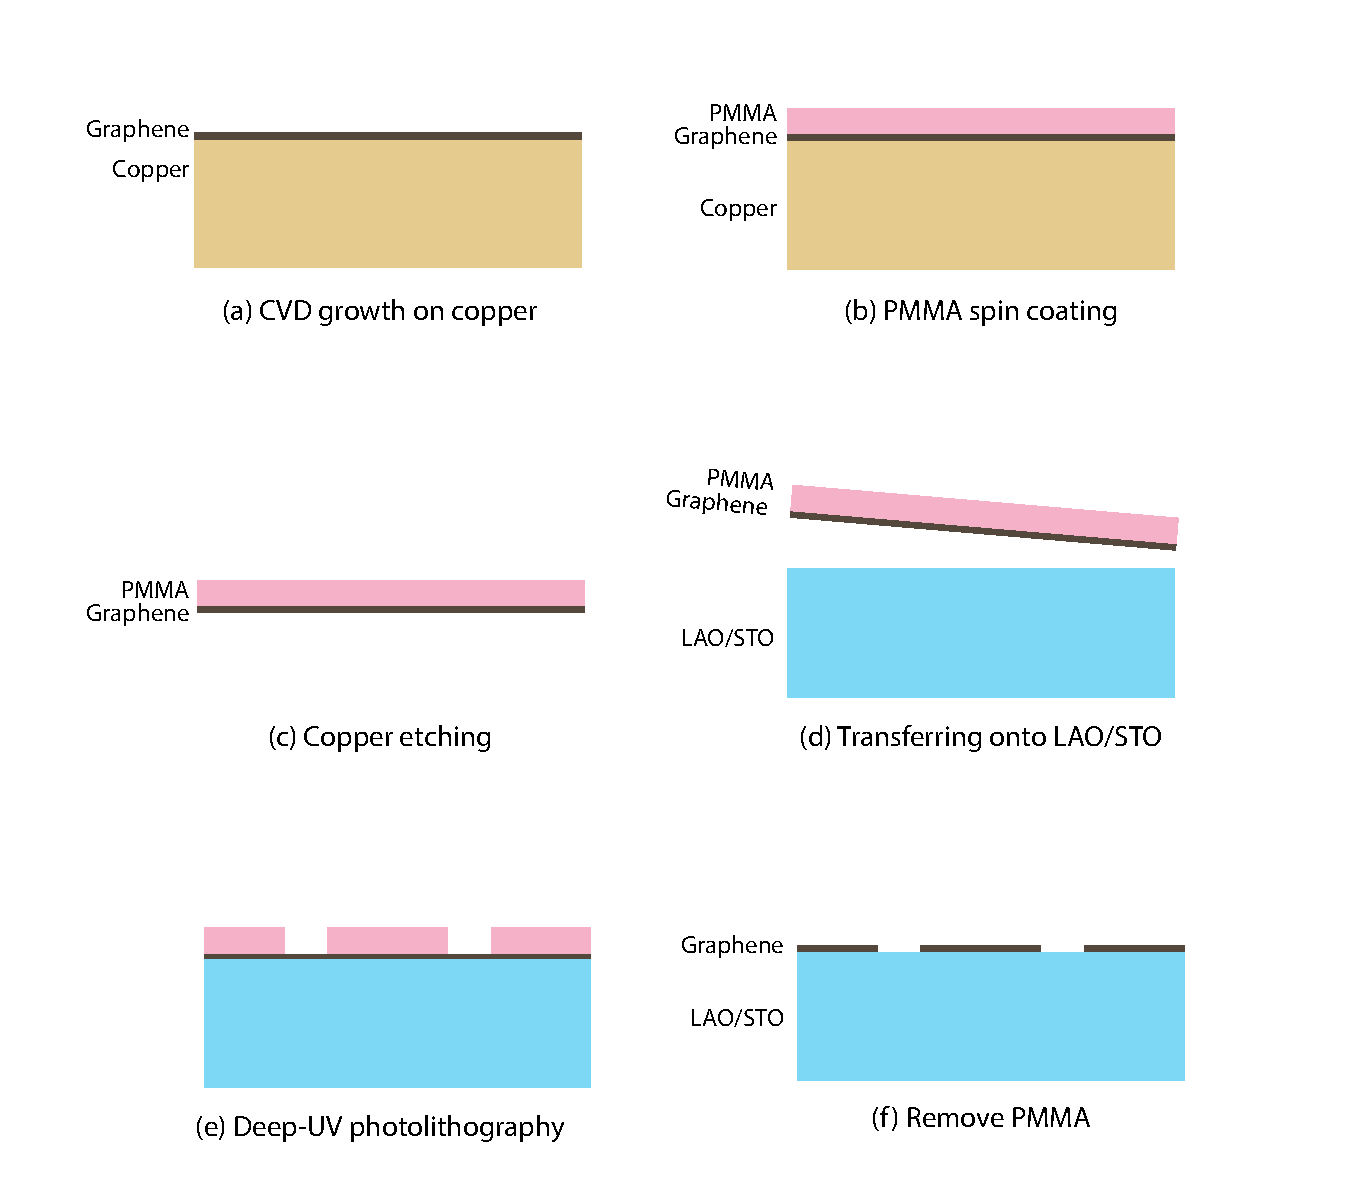
\includegraphics[width=.90\textwidth]{Drawing/PMMATransfer.pdf}
	\caption[CVD graphene transfer and patterning with PMMA]{CVD graphene transfer and patterning with PMMA. (a) Graphene is grown on copper with CVD. (b) PMMA is spin-coated onto the graphene surface. (c) Copper is etched chemically, while graphene floats on the liquid surface. (d) Graphene is transferred onto LAO/STO, using PMMA as a supporting layer. (d) PMMA is patterned with deep-UV lithography. (f) Graphene is etched with oxygen plasma, and then PMMA is removed with the organic solvent.}
	\label{FIG:PMMATransfer}
\end{figure}

The issue with PMMA as a transfer medium is that the residual PMMA is known to be a source of electron scattering, and would significantly reduce the electron mobilities\cite{pirkle2011effect, lin2011graphene, cheng2011toward}. Annealing the sample in H$_2$/Ar environment proves to be able to remove the residue partially, but the process can also introduce structural defects to graphene\cite{lin2011graphene}, or increase coupling between graphene and the substrate and result in deterioration of mobility\cite{cheng2011toward}. 

\begin{figure}[h!]
	\centering
	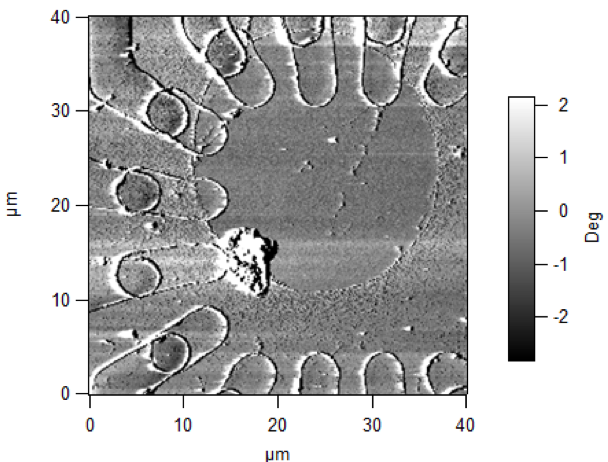
\includegraphics[width=0.60\textwidth]{Drawing/PMMAResidue.png}
	\caption[AFM phase image of graphene on LAO/STO]{AFM phase image of graphene on LAO/STO, transferred with PMMA. The circular region is graphene. Particles can be seen outside graphene, on LAO/STO surface. Other features are the metal electrodes for grahene and interface contact.}
	\label{FIG:PMMAResidue}
\end{figure}

Another drawback of using PMMA as a transfer medium is that the LAO/STO substrate is susceptible to PMMA contaminants. Figure \ref{FIG:PMMAResidue} shows the AFM AC phase image of  LAO/STO with a graphene piece transferred and patterned with PMMA. Graphene covers the inside circle. On the LAO/STO surface, contamination particles can be seen. The experiments in this research require c-AFM writing on the interface; however, most of the LAO/STO samples were found to have lost the interface tunability after the graphene transfer with PMMA\cite{li2016method}. 

A replacement for PMMA is a type of perfluoropolymer Hyflon from Solvay. Our collaborator Dr. Brian D'Urso has used Hyflon for the hydrodynamic experiment, and suggested the possibility of using it for graphene transfer. Hyflon is a type of perfluorinated polymer (similar to Teflon) and is highly hydrophobic and chemically stable. Hyflon has been reported to be widely used in membrane applications such as fuel cells, due to the inertness of C-F bonds\cite{arcella2005hyflon, merlo2007membrane, zhang2012recent}. Thus, unlike PMMA that leaves residue and deteriorates graphene quality, Hyflon can preserve the graphene while used as a transfer medium. Most of the organic or inorganic solvent such as acetone, IPA or DI-water cannot dissolve Hyflon, which makes it a perfect protection layer for graphene. 

The commercially available Hyflon is in powder form. It is only soluble in a few types of perfluorinated solvent. There are different types of Hyflon available, mainly Hyflon AD 40 and Hyflon AD 60, with different molecular weights and phase transition temperature. Although AD 40 has a smaller molecular weight and easier to be dissolved, the sample soft-baking temperature is higher than the phase transition temperature of AD 40 and would cause cross-linking of the polymer chains. The phase transition makes Hyflon AD 40 hard to be removed and affects graphene quality as a result and therefore Hyflon AD 60 is chosen instead.

\subsection{Overview of the Hyflon transfer method}

\begin{figure}[p]
	\centering
	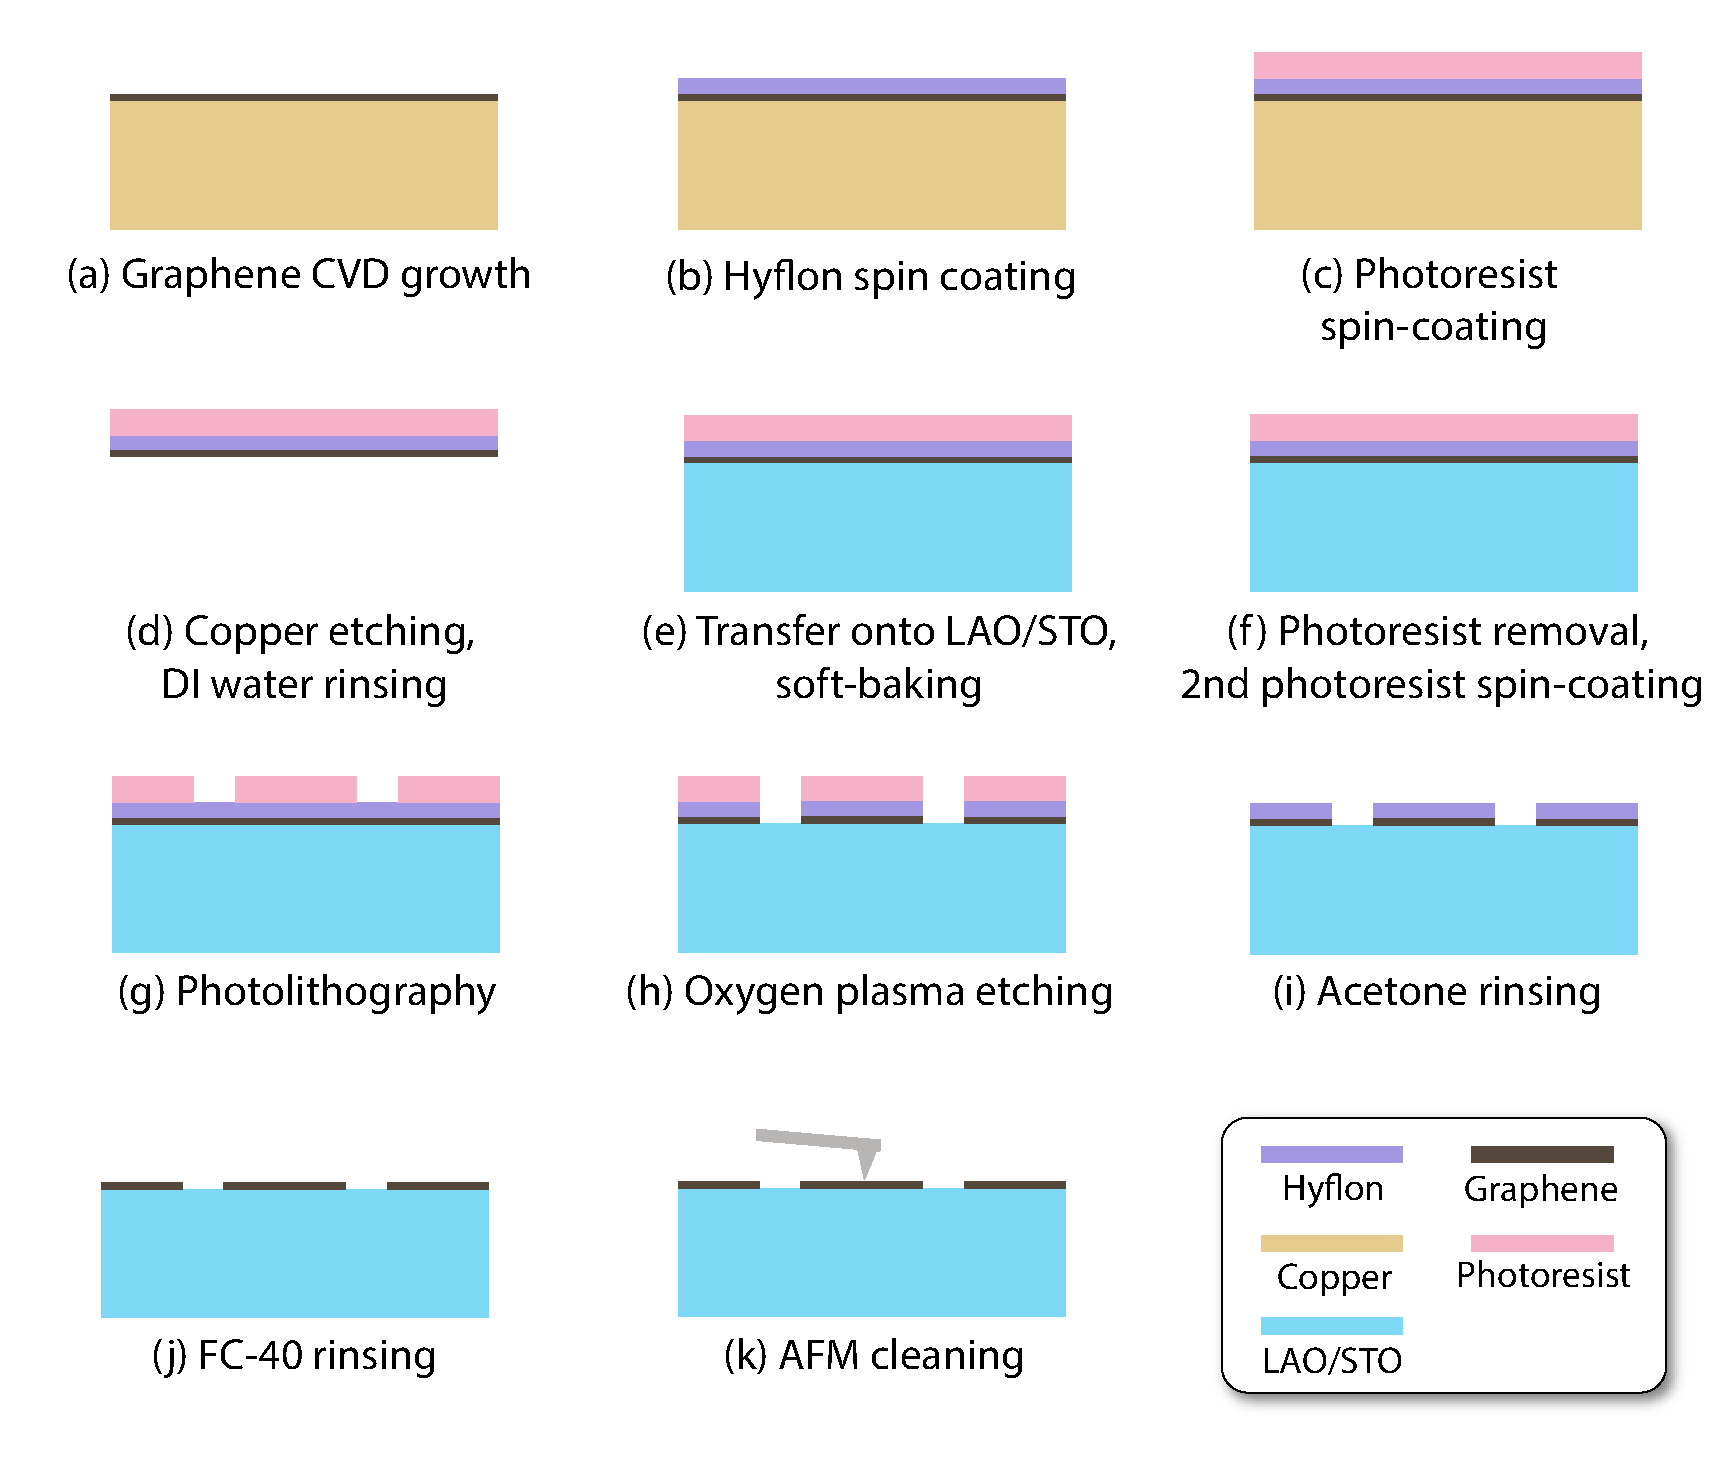
\includegraphics[width=0.9\textwidth]{Drawing/HyflonTransfer.pdf}
	\caption[Hyflon transfer and patterning procedure]{Hyflon transfer and patterning procedure. (a) Graphene is grown with CVD on a copper substrate. (b) Hyflon in spin-coated on graphene. (c) A layer of photoresist is coated on Hyflon as a supporting layer for wet-transfer. (d) Copper substrate is etched with ammonium persulfate; graphene is rinsed in DI-water for several times. (e) Graphene is transferred onto the LAO/STO surface. (f) Photoresist for transfer assistance is removed; another layer of photoresist is coated. (g) Standard UV photolithography. (h) Oxygen plasma etching. (i) Photoresist removal with acetone. (j) Hyflon removal with FC-40. (k) Residue particle cleaning with AFM.}
	\label{FIG:HyflonTransfer}
\end{figure}

The procedure for graphene transfer with Hyflon is similar to the PMMA transfer method. As shown in Figure \ref{FIG:HyflonTransfer}, the graphene on copper is spin coated with Hyflon. The Hyflon film is only 50 nm. Therefore a second supporting layer, photoresist, is spin-coated on top of the Hyflon. The copper is etched with ammonium persulfate while graphene with Hyflon and photoresist floats on the surface of the chemical. The graphene is then rinsed 4 to 5 times and then transferred onto a pre-patterned LAO/STO substrate, and soft-baked to remove the DI water between graphene and LAO. The photoresist is then removed, and another layer of photoresist is spin-coated. The sample is patterned into Hall bars with standard photolithography. Excessive graphene is etched away with oxygen plasma, along with the Hyflon covering it. The patterned graphene/LAO/STO sample is rinsed with acetone to remove the photoresist, and then Hyflon is removed with FC-40. The particles left on the patterned graphene surface is cleaned by AFM in contact mode scans. 

\subsection{Hyflon solution preparation and spin-coating} 

Hyflon solutions in FC-40 are made by adding 2.5 grams of Hyflon powder into 100 ml FC-40. The solution is shaken at 100 rpm for 48 hours. Before spin-coated on the sample, the Hyflon solution needs to go through a series of filters of 450 nm, 200 nm and 100 nm in pore size to remove any undissolved particles. When spin-coated at 3500 rpm, the Hyflon film is about 50 nm in thickness. 

\subsection{Graphene preparation, copper etching, and wet transfer}

\begin{figure}[p]
	\centering
	\includegraphics[width=1.0\textwidth]{Drawing/Transfer.pdf}
	\caption[Hyflon transfer of graphene]{Hyflon transfer of graphene. (a) The graphene with copper foil is cut into squares. The graphene domains can be observed. (b) Copper foil with CVD graphene is fixed onto a silicon wafer as a spin-coating carrier. The edges of the copper foils are carefully sealed with Kapton tape to prevent Hyflon solution leaking into the space between copper and the silicon substrate. (c) After the copper is fully etched by ammonium persulfate, the graphene flake with Hyflon and photoresist floats on the surface of the liquid. (d) Graphene transferred onto pre-patterned LAO/STO. Liquid between the graphene LAO is evaporated in an oven set to 50 $^{\circ}$C or on a hot plate set to 70 $^{\circ}$C.}
	\label{FIG:Transfer}
\end{figure}

The as-grown CVD graphene is on a 100 $\mu$m thick circular copper foil. The LAO/STO substrates that graphene will be transferred on are 5 mm $\times$ 5 mm squares. Therefore, the graphene on copper needs to be cut into 5 mm $\times$ 5 mm shape with a razor blade as shown in Figure \ref{FIG:Transfer}(a). Graphene single domains can be seen in the figure. The square shape copper foil is then fixed onto a 3'' silicon wafer for spin coating. The edges of the graphene need to be carefully sealed so that the Hyflon solution will not leak into the gap between the copper and silicon wafer.

An additional layer of AZ4210 photoresist is spin-coated on Hyflon to assist transferring. However, since the Hyflon is highly hydrophobic, the photoresist solution cannot stick to the surface and form a film of 2.1$\mu$m thick, as it usually does on hydrophilic surfaces. A mild oxygen plasma etching is performed to modify the Hyflon surface and improve surface hydrophilicity. The parameters of plasma etching need to be carefully tuned. In practice, etching the Hyflon for only a few nanometers would drastically improve the hydrophilicity and make photoresist spin-coating possible. Etching the Hyflon for too long might result in damage of graphene, or cross-linking of Hyflon.

After spin coating, the copper foil is taken off the silicon substrate. 1 mol/L concentration ammonium persulfate ((NH$_4$)$_2$S$_2$O$_8$) DI-water solution is prepared beforehand. Ammonium persulfate is a type of oxidation agent widely used as a copper etchant in printed-circuit-board industry. Compared to other chemicals like ferric chloride, ammonium persulfate does not leave metal ion to graphene. The ammonium persulfate solution also needs to go through a 450 nm polymer filter before the etching. Copper etching usually takes 3 -- 4 hours. 

\begin{figure}[h!]
	\centering
	\includegraphics[width=1.0\textwidth]{Drawing/PreClean.pdf}
	\caption[Effect of sample backside clean]{Effect of sample backside clean. (a) Without copper substrate backside cleaning, the graphene transferred onto LAO/STO has contaminant trapped. (b) The graphene on LAO/STO is much cleaner if the backside is cleaned.}
	\label{FIG:PreClean}
\end{figure}

After the graphene transferred onto the LAO/STO, contaminants are sometimes found to be introduced (Figure \ref{FIG:PreClean}(b)). AFM scanning showed that the contaminants were trapped between graphene and LAO. One possibility was that the contaminants were the graphene grown on the back side of the copper. When the copper was etched away by ammonium persulfate, the backside graphene are not detached, and transferred with the topside graphene onto the sample and got trapped between graphene and LAO. 

The \emph{two-step etching} procedure can be used instead. After the copper top surface is coated with Hyflon, it is placed on the surface of the ammonium persulfate solution and left inside an ultrasonic cleaner for 15 minutes. While the backside of the copper is being etched, it is also cleaned by the ultrasound wave so that the backside graphene can be removed. After 15 minutes, the backside is washed by spraying DI-water on it. Then the copper foil is placed back to the surface of ammonium persulfate. After 3 -- 4 hours the copper foil is fully etched, and the graphene with Hyflon and photoresist would float on the liquid surface, as shown in Figure \ref{FIG:Transfer}(c). The graphene flake is then scooped out with a mesh and place on the surface of DI-water for 4 -- 5 times to make sure the ammonium persulfate is washed off the backside of the flake. Then the substrate is slowly lifted towards the flake on the liquid surface and catches the flake. The substrate with the graphene flake on surface is baked in an oven pre-heated to 50 $^{\circ}$C, or on a hot plate at 70 $^{\circ}$C for 5 -- 10 minutes so that the DI-water between graphene and substrate is evaporated, and graphene firmly adheres to LAO (Figure \ref{FIG:Transfer}(d)).

\subsection{Graphene/LAO/STO sample pattern}

The metal electrodes and bonding pads on LAO/STO are patterned before graphene is transferred. Therefore, electrodes are making contacts with graphene from below. The patterns are slightly modified from the one in Section \ref{SEC:AFMLitho}, so that there are electrodes dedicated to making contacts to graphene. As shown in the zoomed-out image in Figure \ref{FIG:GCO}, the graphene Hall bars are located on the canvas for c-AFM lithography. The graphene is in direct contact with the metal electrodes on the LAO/STO surface (orange in color), while LAO/STO is in contact with the interface electrodes (blue). Therefore, the two layers can be measured separately. 

\begin{figure}[p]
	\centering
	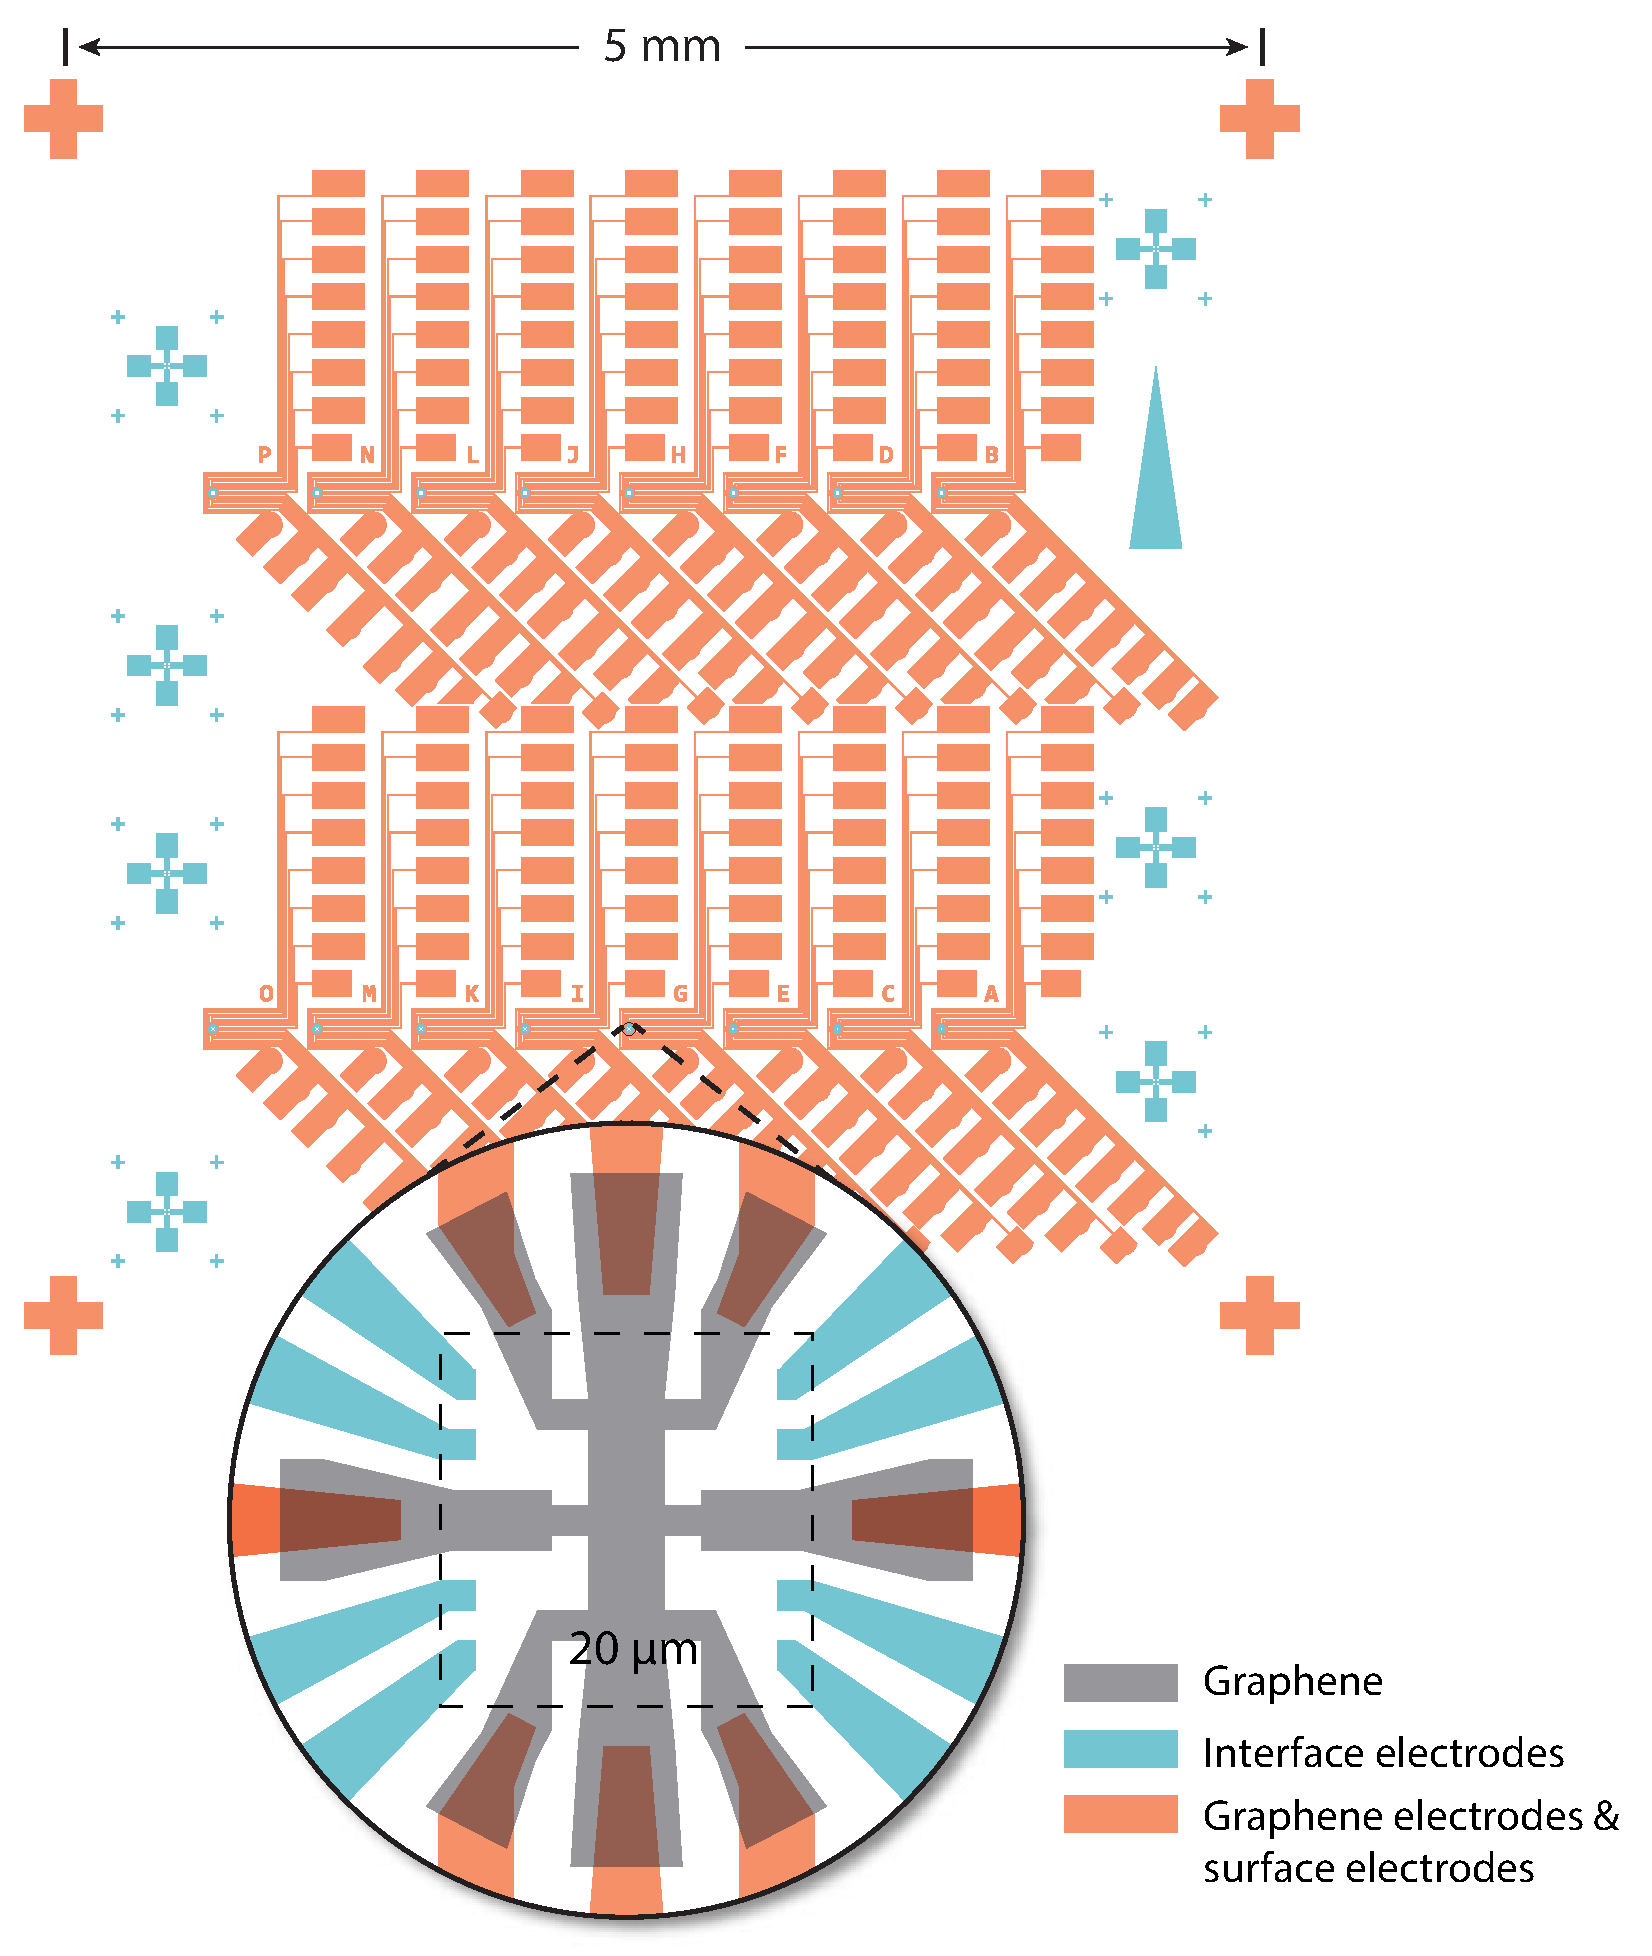
\includegraphics[width=1\textwidth]{Drawing/GCO.pdf}
	\caption[Patterns for graphene/LAO/STO]{Patterns for graphene/LAO/STO. Two sets of electrodes are patterned separately, for interface and graphene contact.}
	\label{FIG:GCO}
\end{figure}

\subsection{Photolithography and etching}

The graphene transferred onto LAO/STO is patterned with standard UV photolithography, as discussed in Section \ref{SEC:Photolithography}. The patterns for graphene Hall bars are inverted, so that the Hall bars are protected by the photoresist and the exposed regions are developed. The oxygen plasma barrel etcher and RIE prove to be effective for graphene and Hyflon etching. The contaminants introduced by a wet-transfer procedure need to be cleaned with RIE as well (Figure \ref{FIG:SampleContaminant}). 

\begin{figure}[p]
	\centering
	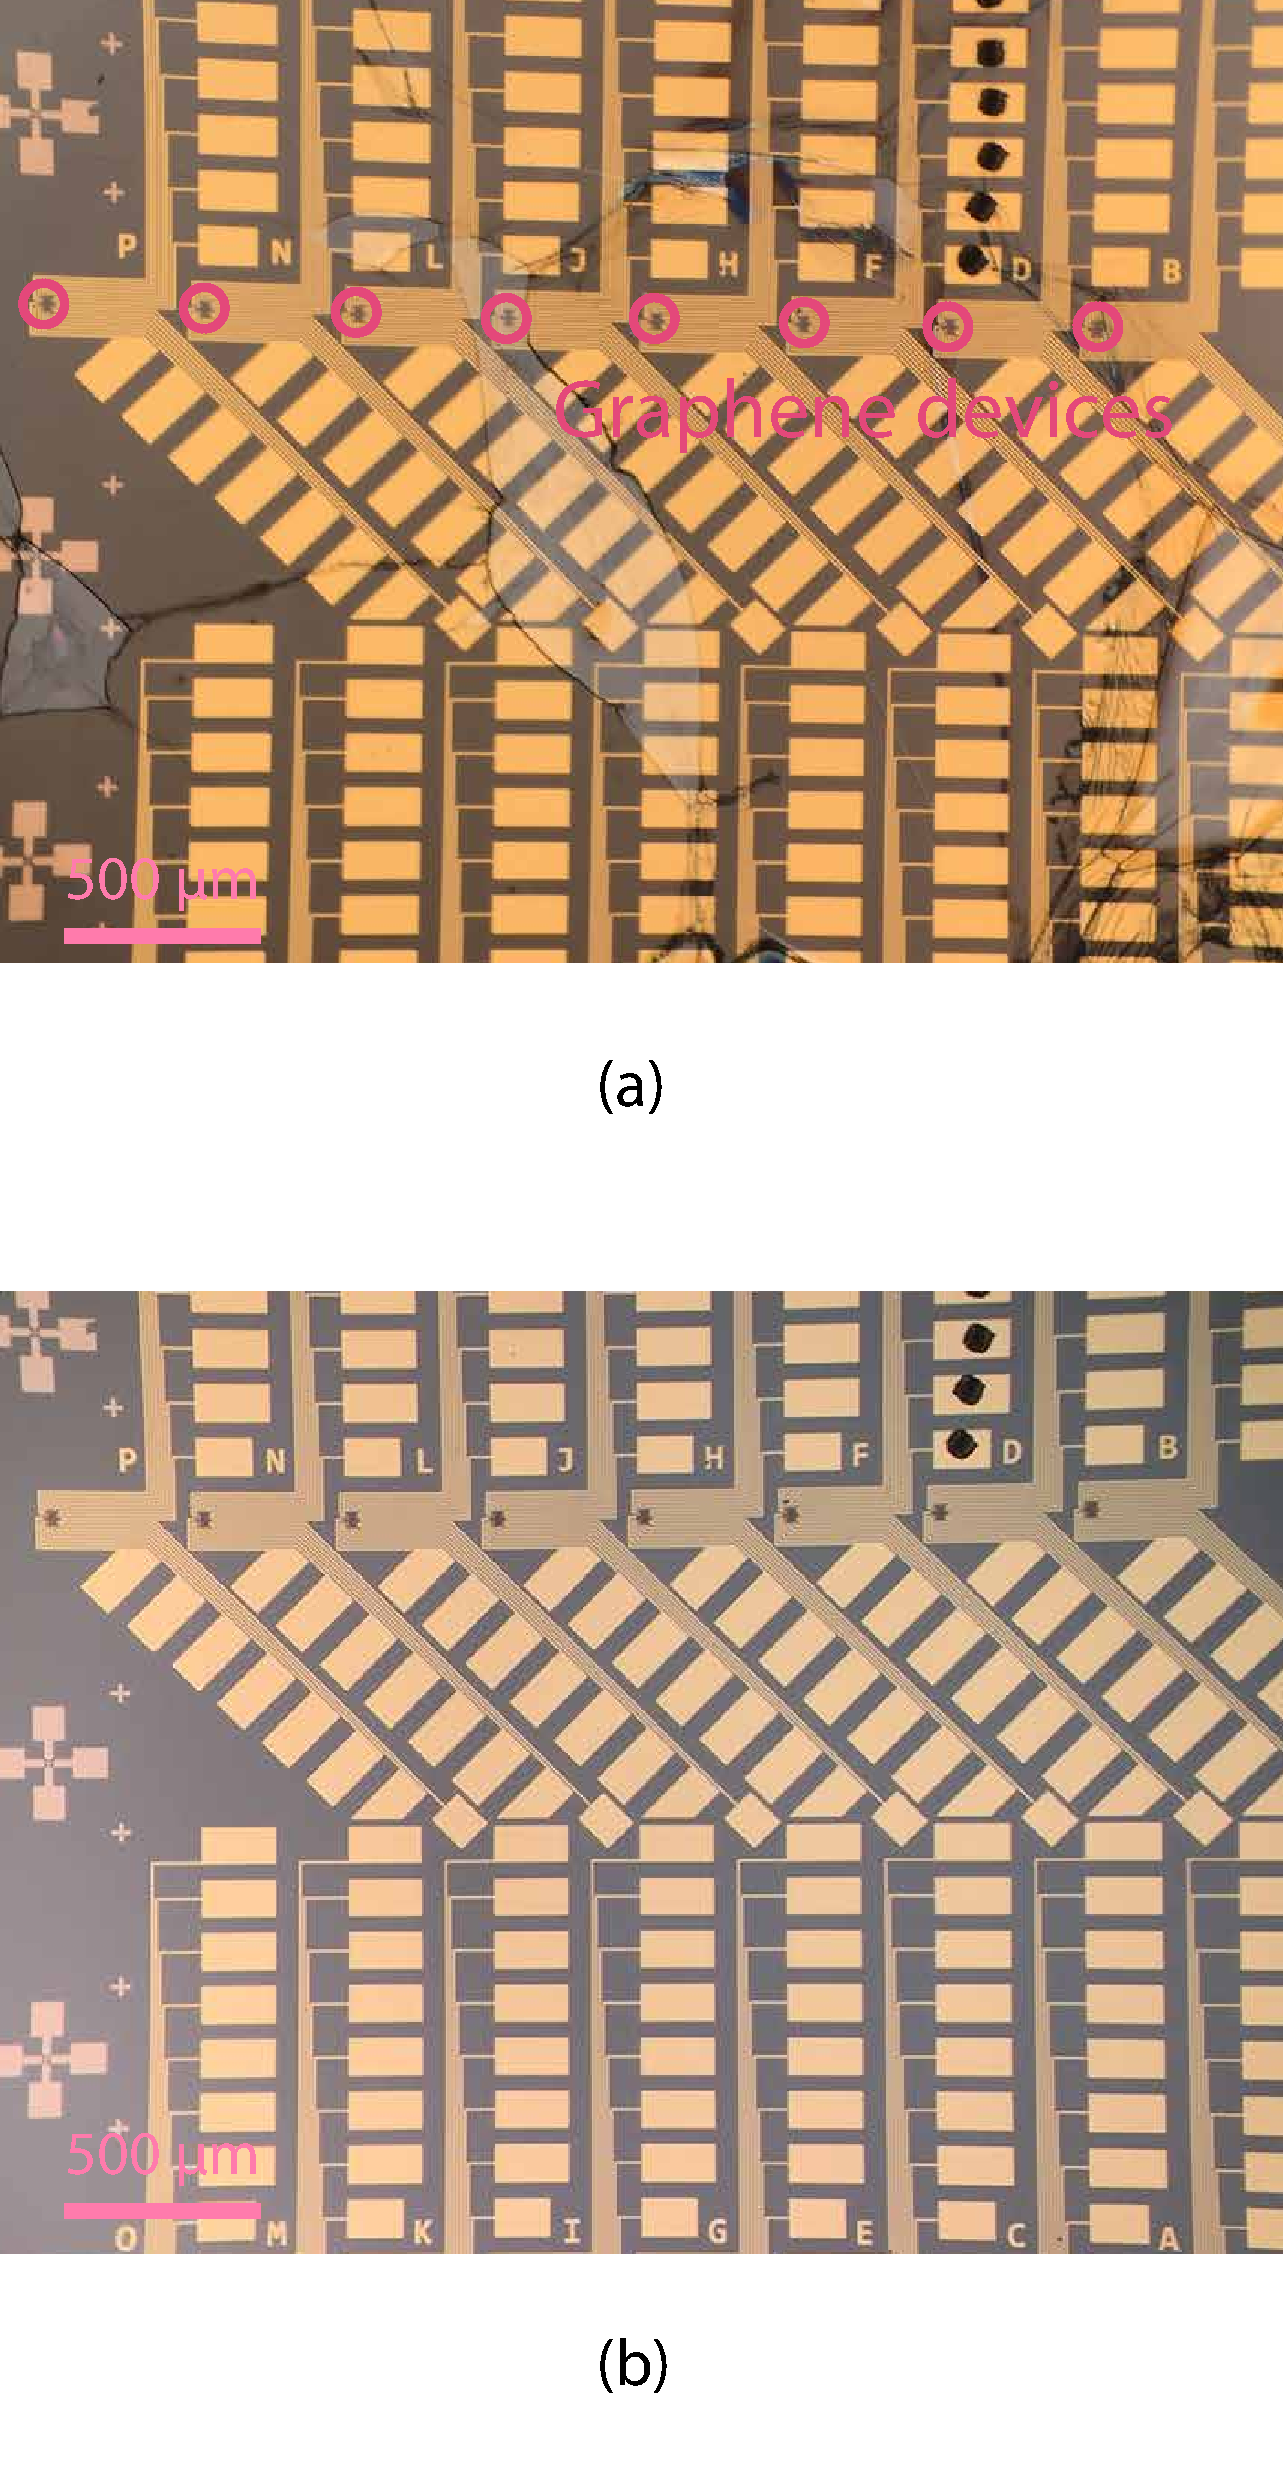
\includegraphics[width=.55\textwidth]{Drawing/SampleContaminant.pdf}
	\caption[Before and after the contaminant etching using RIE]{Before and after the contaminant etching using RIE. (a) Contaminants can be seen after graphene transfer. Only the graphene inside the red circles (zoomed-in image in Figure \ref{FIG:RIEBeforeEtching}) need to be protected with photoresist, and the rest of the graphene can be removed by RIE procedure. (b) The sample surface is clean after the RIE etching.}
	\label{FIG:SampleContaminant}
\end{figure}

\begin{figure}[h!]
	\centering
	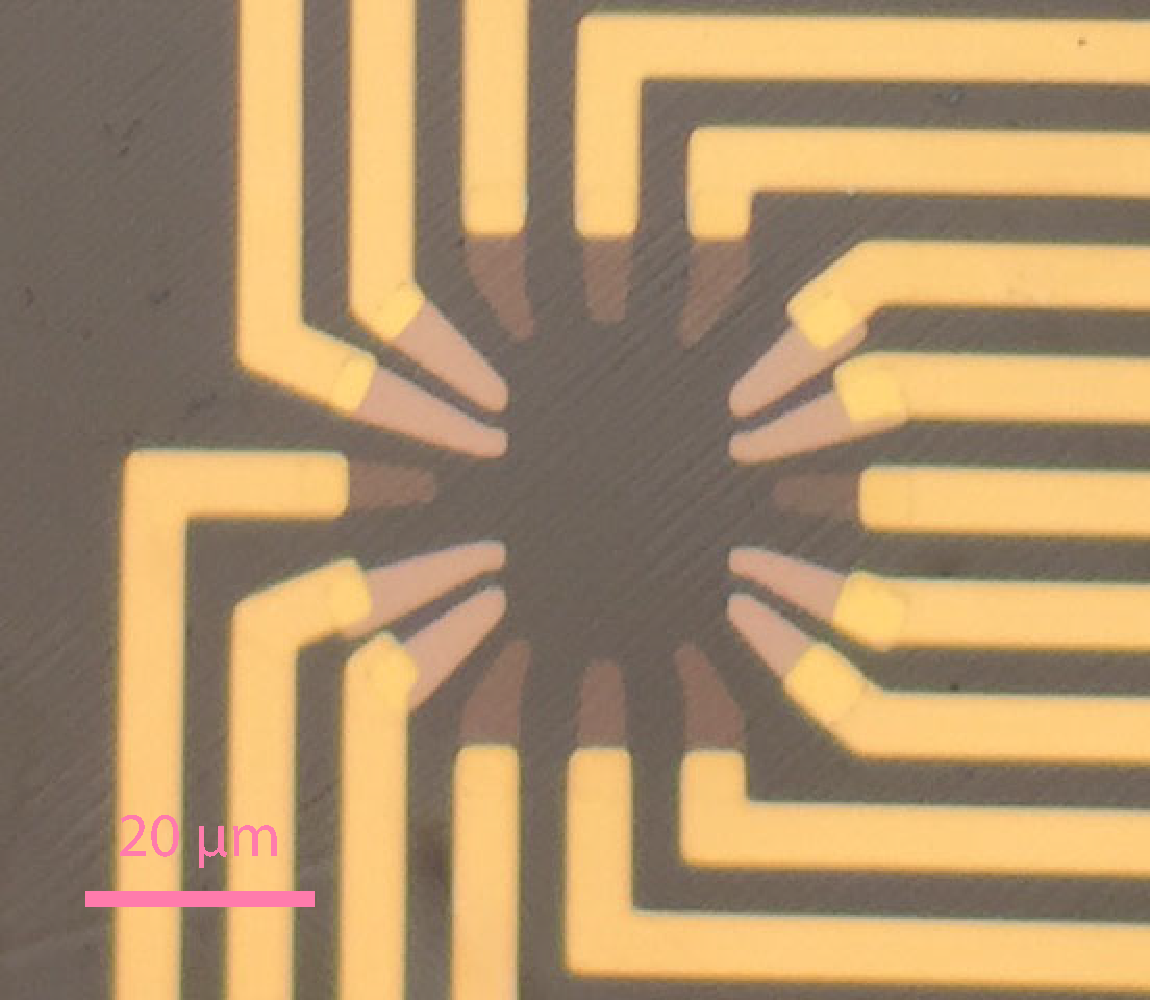
\includegraphics[width=.5\textwidth]{Drawing/RIEBeforeEtching.pdf}
	\caption[The graphene area of interest on pre-patterned LAO/STO sample]{The graphene area of interest on pre-patterned LAO/STO sample. The patterns are for graphene and LAO/STO interface contact.}
	\label{FIG:RIEBeforeEtching}
\end{figure}

\subsubsection{One-step etching}

Before 2018, the the one-step etching method (as shown in Figure \ref{FIG:HyflonTransfer}) was used, that is to etch the graphene and clean the contaminants with RIE in one step. Figure \ref{FIG:SampleContaminant} shows the image of a sample before and after the RIE etching. In Figure \ref{FIG:SampleContaminant}(a), it can be seen that bubbles or foldings introduced from the wet transfer covers the entire sample. To make Hall bars, most of the graphene transferred on LAO/STO needs to be etched away, and only the graphene device inside red circles in Figure \ref{FIG:SampleContaminant}(a) is needed. A zoomed-in image is shown in Figure \ref{FIG:RIEBeforeEtching}, with the graphene covered with Hyflon. The metal patterns are contact electrodes for graphene and the LAO/STO interface. Wrinkles on graphene can also be seen. The contaminants are etched away with an aggressive RIE procedure (listed in Table \ref{TAB:RIESingleStep}). 

\begin{table}
	\centering
	\begin{tabular}{l|c}
		\hline
		Instrument    & RIE \\ \hline
		Gas    &    Oxygen \\ 
		Flow rate    &    19 sccm    \\ 
		Power & 50 W \\
		Pressure    &    300 mTorr    \\
		Time    &    60 -- 180 s \\ \hline
	\end{tabular}
	\caption{One-step RIE etching recipe.}
	\label{TAB:RIESingleStep}
\end{table}

As shown in Figure \ref{FIG:SampleContaminant}(b), the single-step RIE etching can completely clean the contaminants on LAO/STO. However, the etching can also alter the properties of the LAO/STO interface. As shown previously in Figure \ref{FIG:GCO}, the graphene Hall bar locates inside the 20 $\mu$m canvas area. When the graphene outside the Hall bar and surface contaminants are etched with the same aggressive RIE recipe, the bombardment will damage the LAO/STO interface, and it would be impossible to write nanowires with c-AFM in some cases.

\subsubsection{Two-step etching}

\begin{figure}[p]
	\centering
	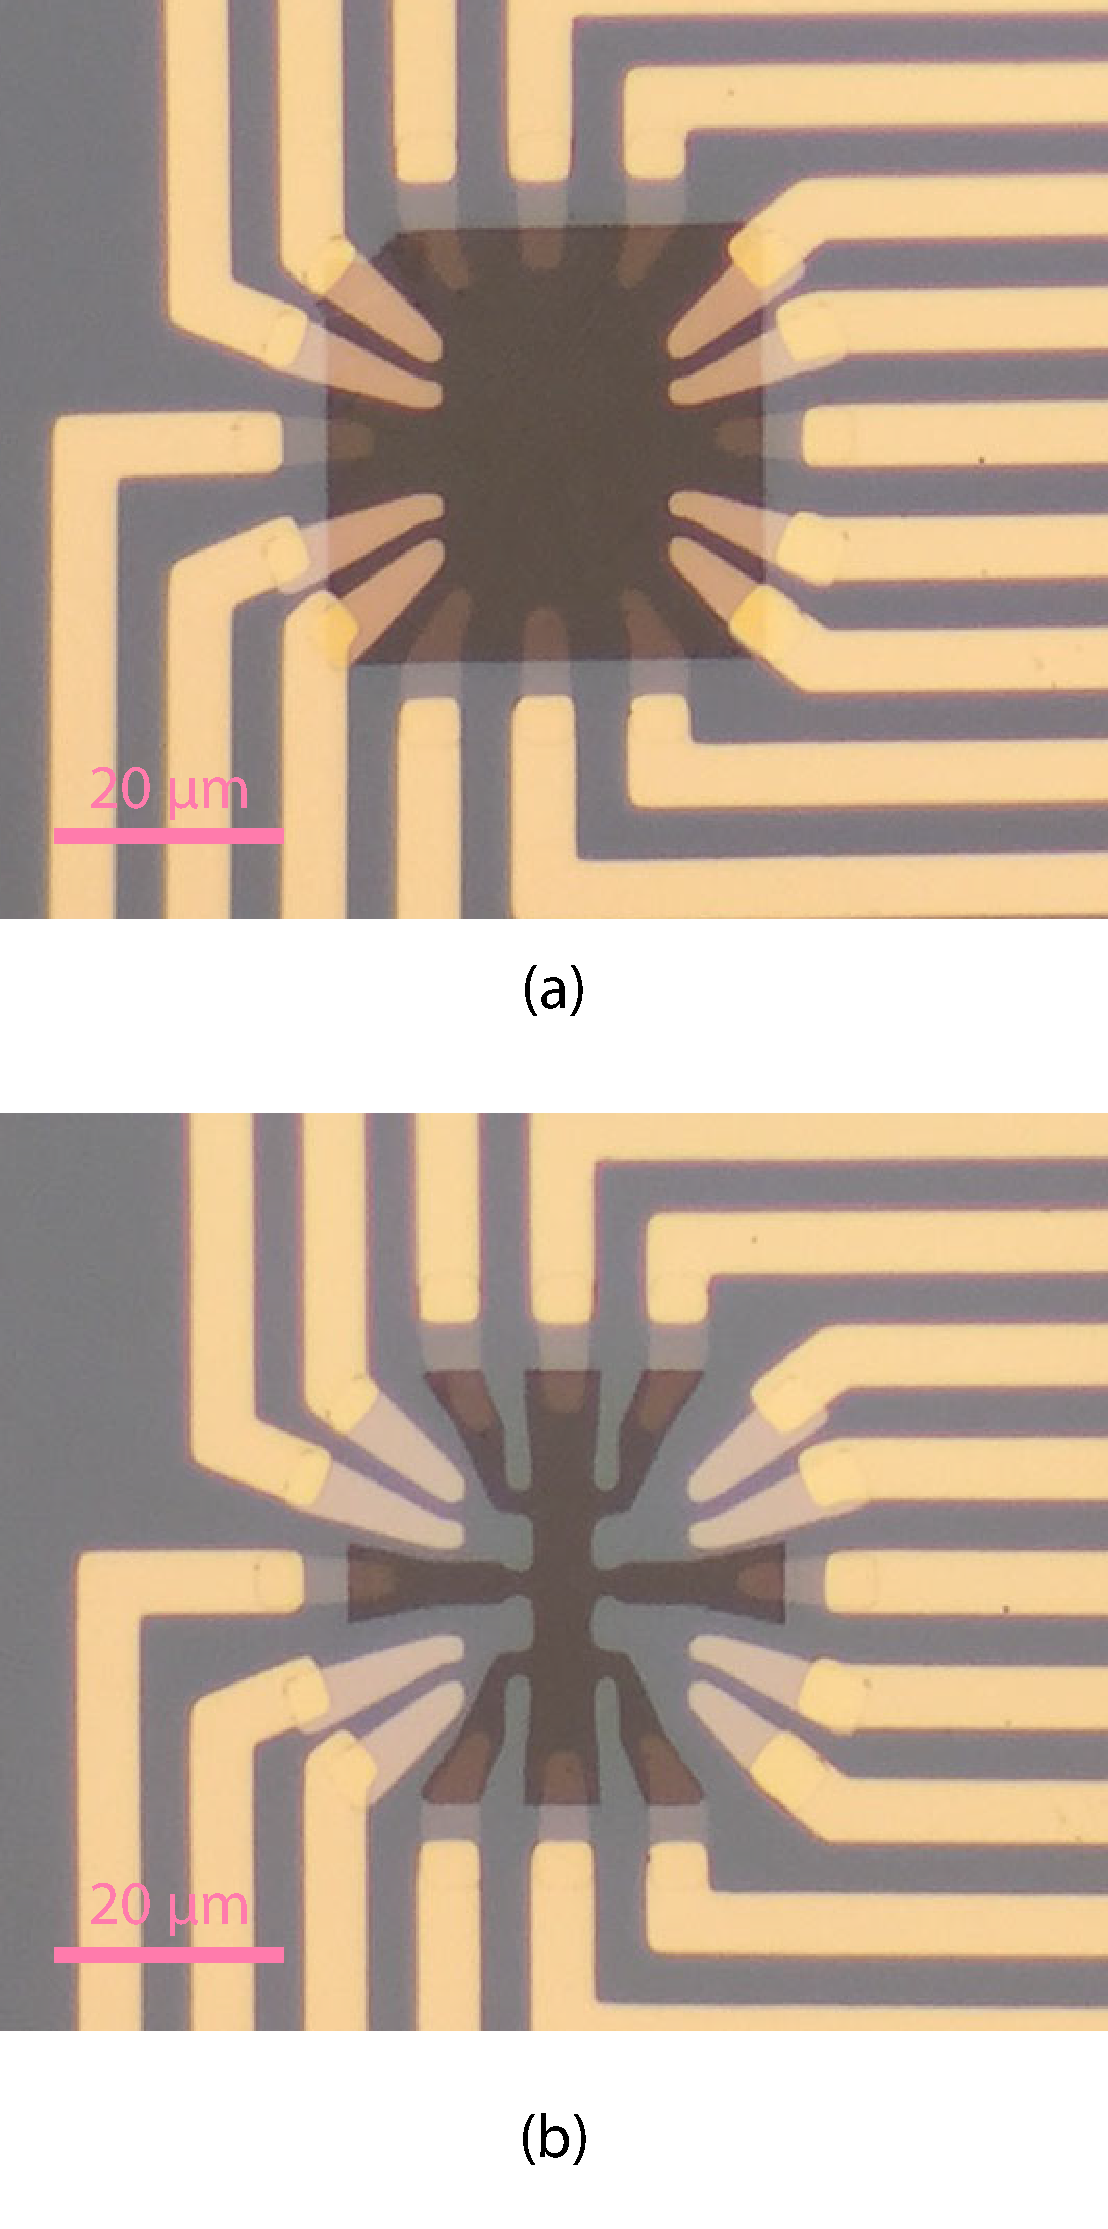
\includegraphics[width=.5\textwidth]{Drawing/RIETwoStep.pdf}
	\caption[Images of two-step graphene etching]{Images of two-step graphene etching. (a) A square shape region is protected by AZ4210 photoresist. Outside of the square region, the sample is etched with an aggressive RIE process to remove the contaminants introduced by wet-transfer. The figure shows the graphene with Hyflon. Photoresist has been washed off. (b) The second step of photolithography is performed, and a Hall-bar shape region is protected by AZ4110 photoresist. Outside of the Hall-bar the Hyflon and graphene are etched away with a mild oxygen-plasma etching recipe, and the LAO/STO interface is still writable. The figure shows the graphene Hall bar covered with Hyflon. }
	\label{FIG:RIETwoStep}
\end{figure}

To address the interface-damaging issue, the two-step etching method is developed for this research. The basic idea is to separate sample cleaning and graphene etching steps. As shown in Figure \ref{FIG:RIETwoStep}. In the first step of etching, the Hyflon and graphene are protected by photoresist in a square shape, that covers the Hall bar devices to be patterned in the next step and the LAO/STO canvas region. The rest of the sample is etched with an aggressive RIE recipe so that the contaminants on bonding pads and connection patterns are entirely removed. After the etching, the photoresist is washed away with acetone and IPA. In the second step, another layer of photoresist is spin-coated and patterned into graphene Hall-bar device shape. Then the graphene and Hyflon outside the Hall bar region but covering the LAO/STO canvas are etched away with a much weaker oxygen plasma so that the graphene and Hyflon is etched while the LAO/STO interface is not damaged.

\begin{figure}[p]
	\centering
	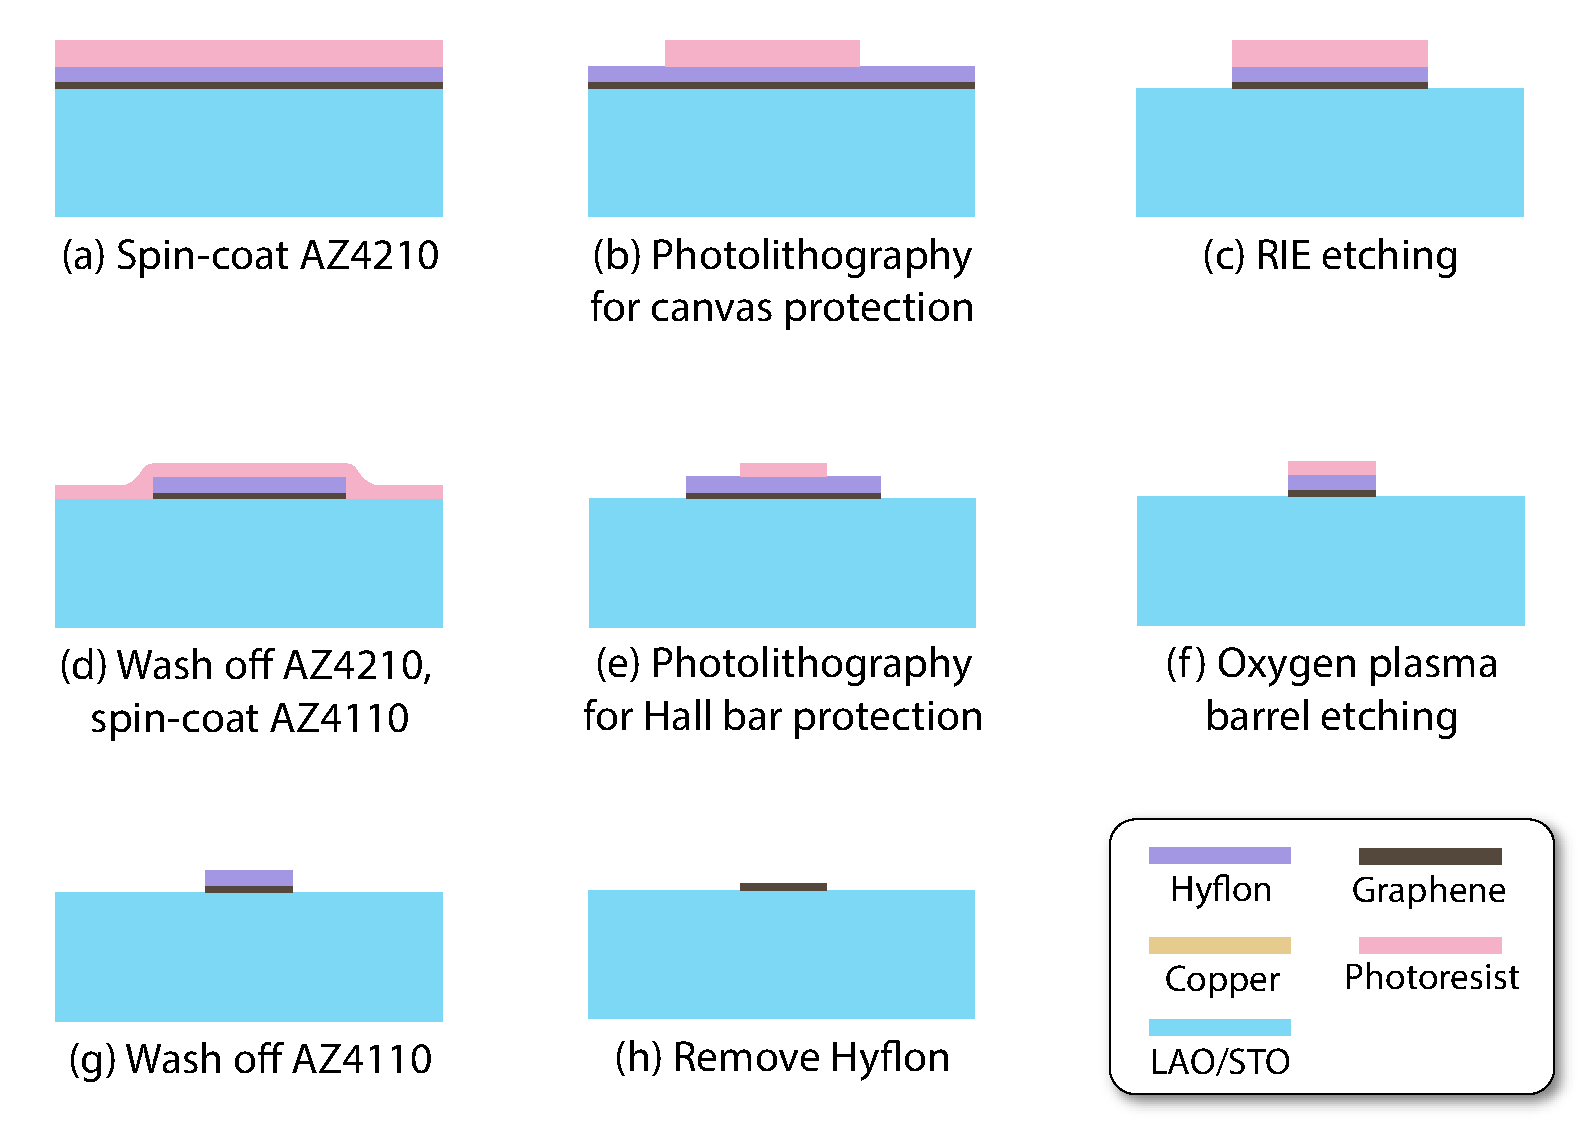
\includegraphics[width=.75\textwidth]{Drawing/TwoStepEtching.pdf}
	\caption[Procedures of two-step graphene etching]{Procedures of two-step graphene etching. (a) AZ4210 is spin-coated on Hyflon. (b) The photoresist is patterned into a square-shape protection layer for the canvas. (c) An aggressive RIE process is used to fully remove the contaminants outside the canvas. (a) to (c) might be repeated if necessary. (d) AZ4110 is spin-coated. (e) Hall-bar shape is patterned using photolithography, to protect the Hyflon and graphene on the regions of interest. (f) A weak oxygen plasma etching step is used to remove the unwanted Hyflon and graphene. (g) AZ110 is washed off by solvents. (h) Hyflon is removed by FC-40.}
	\label{FIG:TwoStepEtching}
\end{figure}

The detailed procedures are shown in Figure \ref{FIG:TwoStepEtching}. Right after graphene is transferred onto LAO/STO and the supporting photoresist is washed off, the sample is spin-coated with AZ4210. The square-shape is patterned with photolithography to protect the canvas. Then the sample is etched with RIE, until all the contaminants are cleaned. In some cases, the contaminants need long etching time ($> 300$ seconds), and photoresist may be etched through. Multiple photolithography and RIE etching steps will be needed.
For the same reason, AZ4210 (2.1 $\mu$m thick) is preferred than AZ4110 (1.1 $\mu$m thick). After the RIE cleaning, AZ4210 is washed off, and AZ4110 is spin-coated. The Hall bar is patterned on AZ4110, and then the graphene and Hyflon are shaped into Hall bars (Figure \ref{FIG:RIETwoStep}). The recipes for photolithography and etching are listed in Table \ref{TAB:TwoStepPL} and Table \ref{TAB:TwoStepEtching}.

\begin{table}
	\centering
	\begin{tabular}{l|cc}
		\hline
		Photoresist    & AZ4210 (step 1) & AZ4110 (step 2) \\ \hline
		Spin-coating    &    4000 rpm    &    4000 rpm \\ 
		Baking    &    95 $^{\circ}$C    &    95 $^{\circ}$C    \\ 
		UV dose    &    170 mJ    &    100 -- 120 mJ    \\
		Developer : DI-water    &    1 : 4 &    1 : 4 \\ 
		Developing time    &    120 s    &    240 -- 600 s \\
		\hline
	\end{tabular}
	\caption[Two-step etching photolithography recipe]{Two-step etching photolithography recipe. First layer of AZ4210 is used to protect the canvas against the aggressive RIE for contamination removal. Second layer of AZ4110 is for graphene Hall bar protection, and only need to resist a mild oxygen-plasma etching.}
	\label{TAB:TwoStepPL}
\end{table}

\begin{table}
	\centering
	\begin{tabular}{l|cc}
		\hline
		Instrument    & RIE (step 1)    &    Barrel etcher (step 2) \\ \hline
		Gas    &    Oxygen &    Oxygen \\ 
		Pressure    &    300 mTorr    &    $\sim$ 600 mTorr \\
		Power    &    50 W    &    100 W \\
		Time    &    200 -- 400 s &    300 s\\ \hline
	\end{tabular}
	\caption[Two-step etching recipe]{Two-step etching recipe. Although the barrel etcher runs at a higher power, the etching much less invasive compared to RIE.}
	\label{TAB:TwoStepEtching}
\end{table}

\subsection{Hyflon removal}

Over the entire processing, the graphene is covered with Hyflon until the last step. The Hyflon is only solvable in the perfluorinated solvent such as FC-40. Two recipes are used for Hyflon removal. 

\subsubsection{High temperature method} FC-40 is heated up to 165 $^{\circ}$C in a beaker, lower than the boiling point 175 $^{\circ}$C. Once the sample is placed in FC-40, the liquid start to be shaken at 100 rpm for 12 hours while it cools down to room temperature.

\subsubsection{Low temperature method} FC-40 is heated up to 70 $^{\circ}$C in a beaker. After the sample is immersed in FC-40, the beaker is shaken at 100 rpm while the temperature is kept at 70 $^{\circ}$C for 12 -- 24 hours.

\subsection{AFM cleaning of graphene}

All the solvents including DI-water, IPA, and FC-40 leave a layer of nano-particles on the sample surface, until the sample is cleaned by oxygen plasma. For graphene/LAO/STO sample, even a weak recipe of oxygen plasma etching can potentially cause structural damage to the graphene. Therefore, the nano-particles from solvents and Hyflon are cleaned with AFM contact mode scanning, as a final step of processing. 

\begin{figure}[p]
	\centering
	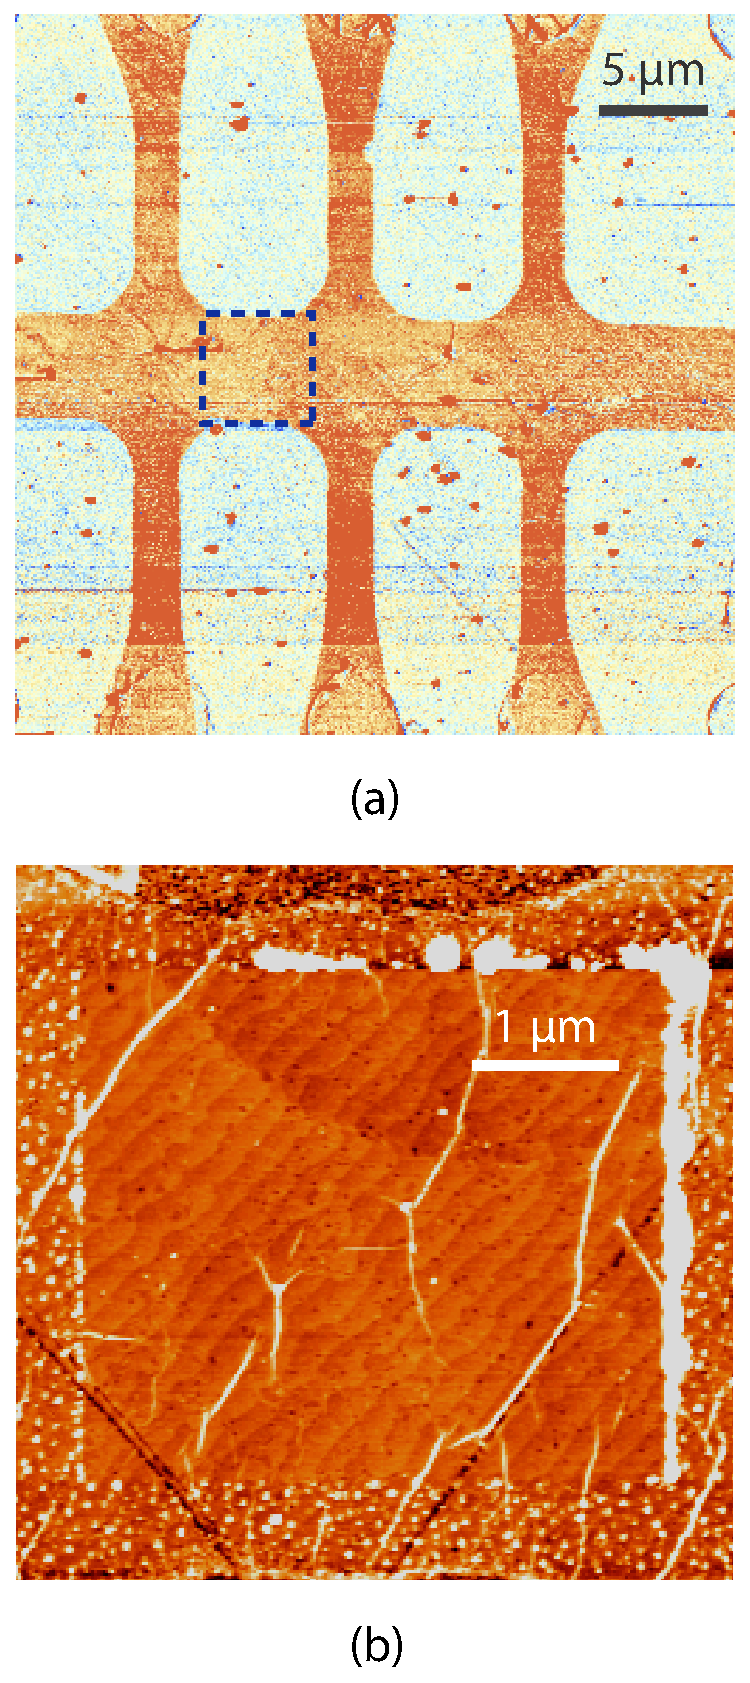
\includegraphics[width=0.4\textwidth]{Drawing/GrapheneAC.pdf}
	\caption[AFM cleaning of graphene]{AFM cleaning of graphene. (a) The organ Hall bar region is the graphene, after Hyflon removal in FC-40. Particles on graphene can be observed. (b) Zoomed-in image of the square region in (a). The center has been scanned in AFM contact mode. Particles are pushed to the top and right edges. Terraces of LAO/STO and wrinkles can be observed.}
	\label{FIG:GrapheneAC}
\end{figure}

Figure \ref{FIG:GrapheneAC} shows the AFM images of graphene before and after cleaning. Figure \ref{FIG:GrapheneAC}(a) is the AFM AC mode phase image. The Hall bar shape in orange is the graphene, and the LAO surface is in cyan color. Particles of various sizes can be observed on the entire sample. Larger particles ($\sim$ 100 nm) are probably from the FC-40, while the smaller particles ($<$ 100 nm) are the residues of Hyflon. Figure \ref{FIG:GrapheneAC}(b) is the zoomed-in image of the squared region in \ref{FIG:GrapheneAC}(a), after the center is been scanned with AFM in contact mode. Particles are pushed to the edges of the square. Inside the scanned region, terraces ($h = 4 \ \mathrm{\AA}$) of the LAO/STO substrate can also be observed. Wrinkles of the graphene are formed during the transfer, or the AFM contact scan. Normally the mechanical strength of graphene is high enough\cite{lee2008measurement} to withstand the scanning with a contact force of 100 nN. However, if the raster scan is too fast while the graphene is covered with a large amount of contaminant, or while the tip is scanning from the LAO to graphene from the edge, the graphene can still be broken. Typical cleaning recipes used in this research are listed in Table \ref{TAB:AFMCleaning}.

\begin{table}[h!]
	\centering
	\vspace{0.85cm}
	\begin{tabular}{l|cc}
		\hline
		AFM model    &    Asylum MFP3D    &    Asylum Cypher \\ \hline
		Tip spring constant    &    3 N/m    & 3 N/m    \\ 
		Deflection set-point    &    0.05 -- 0.5 V    &    0.1 -- 1.0 V    \\        
		Contact force    &    40 -- 400 nN    &    20 -- 200 nN    \\
		Scanning speed    &    10 $\mu$m/s    &    10 $\mu$m/s \\ 
		Line separation    &    10 -- 20 nm    &    10 -- 20 nm    \\ \hline
	\end{tabular}
	\caption{Graphene cleaning recipes on Asylum MFP3D and Cypher.}
	\label{TAB:AFMCleaning}
	
\end{table}

\begin{figure}[h!]
	\centering
	\vspace{0.85cm}
	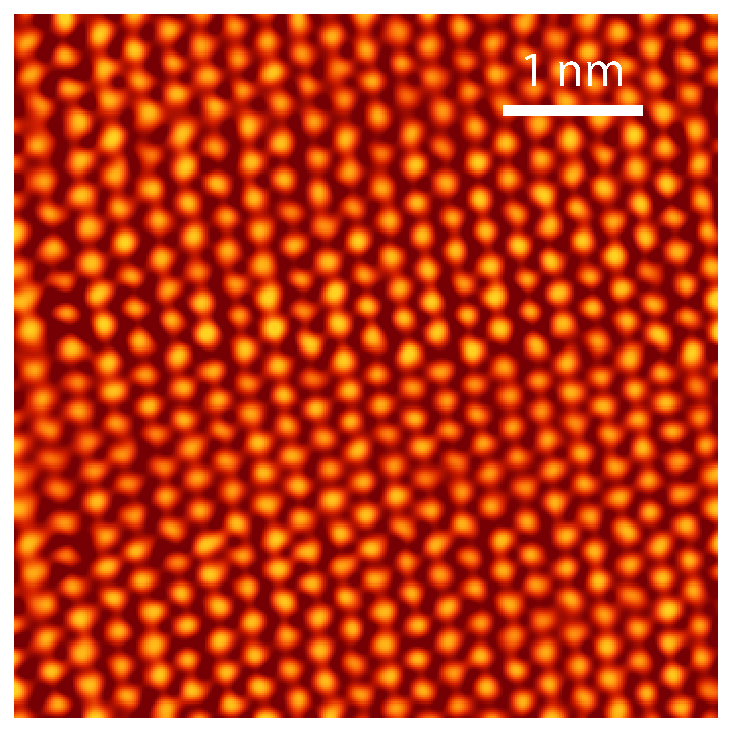
\includegraphics[width=0.45\textwidth]{Drawing/GrapheneSTM.pdf}
	\caption[STM image of graphene on LAO/STO after AFM cleaning]{STM image of graphene on LAO/STO after AFM cleaning.}
	\label{FIG:GrapheneSTM}
\end{figure}

A room temperature STM measurement is performed after AFM cleaning. Tunneling currents are measured from the graphene surface to a tungsten STM tip. From the STM image the graphene atoms can be identified.

\subsection{Graphene/LAO/STO nano-scale device writing}

The experiments on graphene, such as Klein tunneling\cite{allain2011klein, katsnelson2006chiral, young2009quantum, shytov2008klein}, edge state mixing\cite{williams2007quantum, abanin2007quantized, lohmann2009four, amet2014selective}, band structure engineering using superlattice\cite{forsythe2018band}, rely on the Dirac-like band structure and tunability of carriers from electrons to holes. The ability to tune the CNP is central to controlling these exotic properties of graphene. c-AFM writing is proved to be a powerful tool to create nanostructures on LAO/STO interfaces. Pattern nano-scale devices on graphene/LAO/STO reversibly with c-AFM is one of the major techniques this research is focusing on. 

\subsubsection{c-AFM writing and PFM imaging}
\begin{figure}[p]
	\centering
	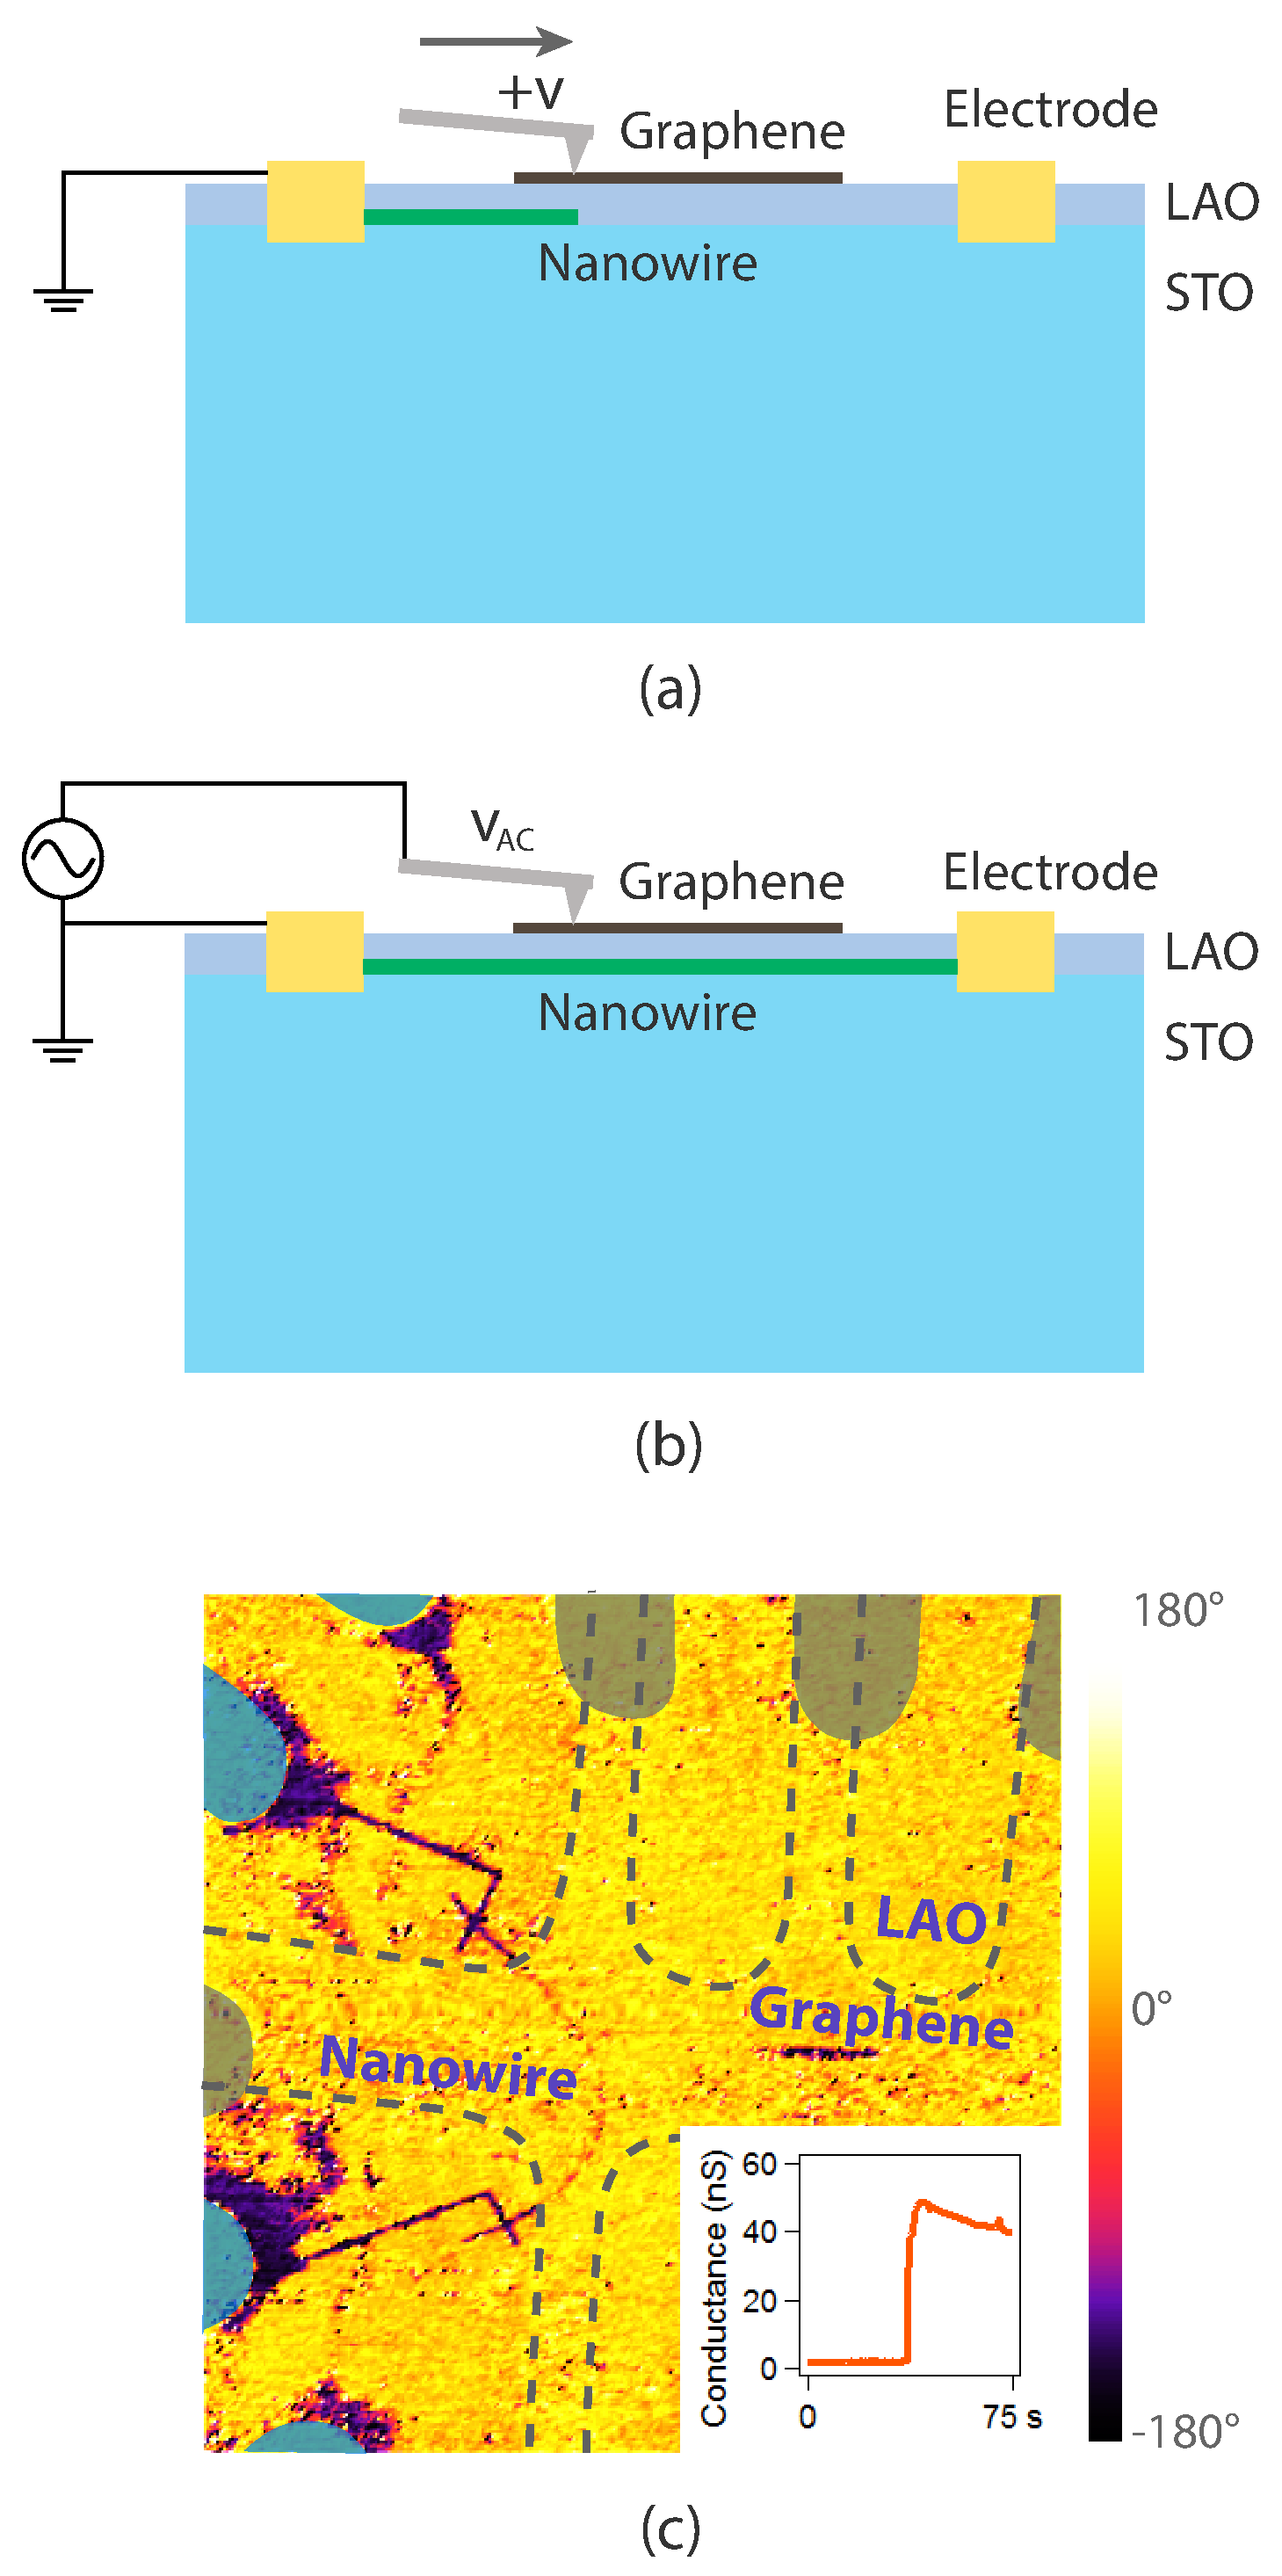
\includegraphics[width=0.55\textwidth]{Drawing/GraphenePFM.pdf}
	\caption[Writing and imaging of the graphene/LAO/STO nanowire]{(a) Writing and imaging of the graphene/LAO/STO nanowire. c-AFM writing of graphene/LAO/STO nanowire. (b) PFM measurement setup. (c) PFM image of the nanowire on LAO/STO interface, underneath the graphene. The inset shows the sudden jump of conductance after the two interface electrodes are connected.}
	\label{FIG:GraphenePFM}
\end{figure}

Figure \ref{FIG:GraphenePFM}(a) demonstrates the setup of c-AFM writing on graphene/LAO/STO. The conductance between two interface electrodes are measured \textit{in situ} during the writing process. A positive voltage $V_\mathrm{tip} > +6$ V is applied to the c-AFM tip, while the tip sketches on the sample surface. A protective resistor of 1 G$\Omega$ is connected between the tip and voltage source (not shown in Figure \ref{FIG:GraphenePFM}). The graphene is disconnected and the potential is floating. The tip sketches through the graphene-covering area before two interface electrodes are connected. The typical voltage applied to the AFM tip is $+15$ V, and the tip sketching speed is 0.5 -- 1 $\mu$m/s. The contact force between the tip and sample is 20 -- 80 nN. A sudden increase of conductance between two electrodes can be observed (inset of Figure \ref{FIG:GraphenePFM}(c)) when a conductive channel is created. 

The nanowire on the LAO/STO interface is imaged using PFM. A sinusoidal bias voltage (with the frequency close to the PFM resonance frequency of the sample) is applied to the c-AFM tip, while the tip is in contact with the sample. The bias voltage modulates the carrier density on the LAO/STO interface, and causes deformation of STO through the Jahn-Teller effect\cite{huang2013direct, vonk2007interface, salluzzo2009orbital, park2006charge}. The nanowire has a different carrier density from the rest of the sample and is visible in the PFM image (Figure \ref{FIG:GraphenePFM}(c)). The region colored in blue are the interface electrodes, and the area in gray are the electrodes to graphene. The graphene covered areas are outlined with dashes. The narrow path in dark purple is the nanowire written with c-AFM. The path under the graphene is dimmer than the rest of the wire, possibly from the shielding effect of graphene.

\subsubsection{c-AFM writing conditions on graphene/LAO/STO and graphene damage thresholds}

As discussed in section \ref{SEC:AFMLitho}, c-AFM nanowire writing and erasing relies on the water-cycle mechanism. The surface conditions of LAO can also affect the interface 2DEG\cite{brown2016giant, xie2011control, xie2013enhancing, aliaj2018probing}. It has been reported\cite{alaboson2011conductive} that the graphene can be damaged at tip voltages $>$ 6 V. In this research, it is found that the damage threshold depends on whether the graphene is floating or grounded, and the current flowing from graphene to the tip. Figure \ref{FIG:GrapheneDamages} is an AC phase image of the damaged graphene. The light color paths show the oxidized graphene. In this research, the tip voltage is limited to $-5$ V when the graphene is grounded, and $-8$ V when the graphene is floating while performing c-AFM on graphene with a negative voltage. The c-AFM writing/erasing parameters are listed in Table \ref{TAB:GCOLithography}.

\begin{table}[h!]
	\centering
	\vspace{0.85cm}
	\begin{tabular}{l|cc}
		\hline
		&    Writing    &    Erasing \\ \hline
		Tip spring constant    &    3 N/m    & 3 N/m    \\ 
		Deflection set-point    &    0.05 -- 0.5 V    &    0.1 -- 1.0 V    \\    
		Tip voltage    &    $+10$ V -- $+20$ V    & $-$5 V (graphene grounded) \\
		&    & $-$8 V (graphene floating) \\
		Contact force    &    80 nN    &    80 nN    \\
		Tip speed    &    0.4 -- 10 $\mu$m/s    &    0.4 -- 10 $\mu$m/s \\ \hline 
	\end{tabular}
	\caption{c-AFM writing and erasing parameters on graphene/LAO/STO samples.}
	\label{TAB:GCOLithography}
\end{table}

\begin{figure}[h!]
	\centering
	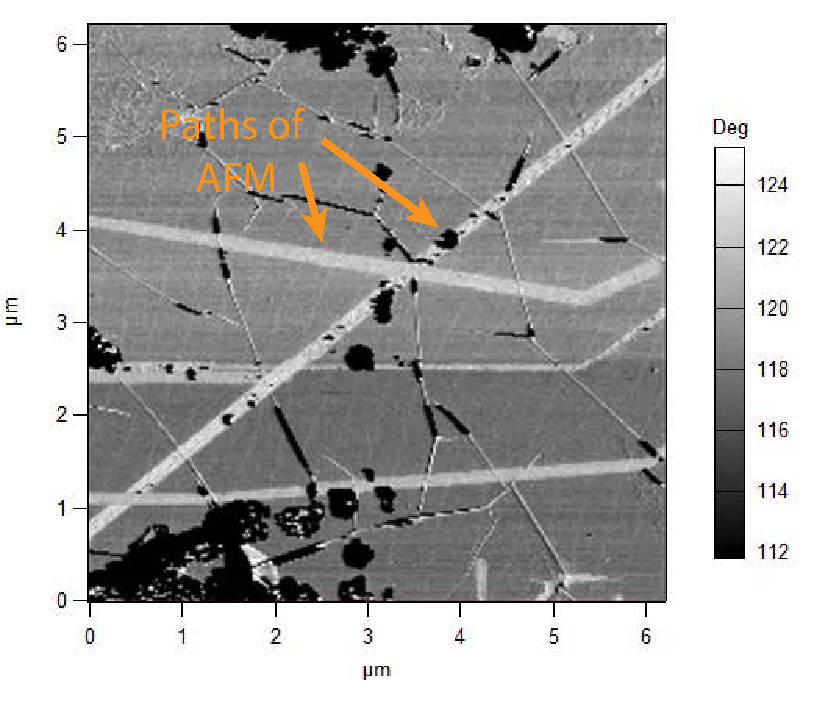
\includegraphics[width=.7\textwidth]{Drawing/GrapheneDamages.pdf}
	\caption[AC phase image of damaged graphene from c-AFM writing]{AC phase image of damaged graphene from c-AFM writing.}
	\label{FIG:GrapheneDamages}
\end{figure}

\chapter{Graphene/LAO/STO heterostructure device}
\label{SEC:GCO}

This chapter is about the transport properties of graphene device on graphene/LAO/STO. Graphene CNP can be reversibly controlled with c-AFM writing technique, similar to the nanostructure lithography on bare LAO/STO. Two experiments are discussed in details: edge-state mixing on graphene $p$-$n$ junctions and graphene superlattice patterning. The measurements are performed at $T = 2$ K, above the critical temperature for superconductivity in LAO/STO interface. This project is in collaboration with Qing Guo from University of Pittsburgh.

\section{Transport measurement in graphene}

Figure \ref{FIG:HallDevice} illustrates the typical geometry of graphene/LAO/STO devices. The graphene on LAO/STO is patterned into Hall bar shapes. Gold electrodes make contact with the graphene from the surface of LAO. The bottom of the sample is pained with silver epoxy, and the backgate voltage is applied to the bottom to control the global chemical potential of graphene. Current flows through the main channel of graphene, with a typical $I = 100$ nA. Longitudinal and transverse voltages are measured from the leads shown in Figure \ref{FIG:HallDevice}(b).

\begin{figure}[p]
	\centering
	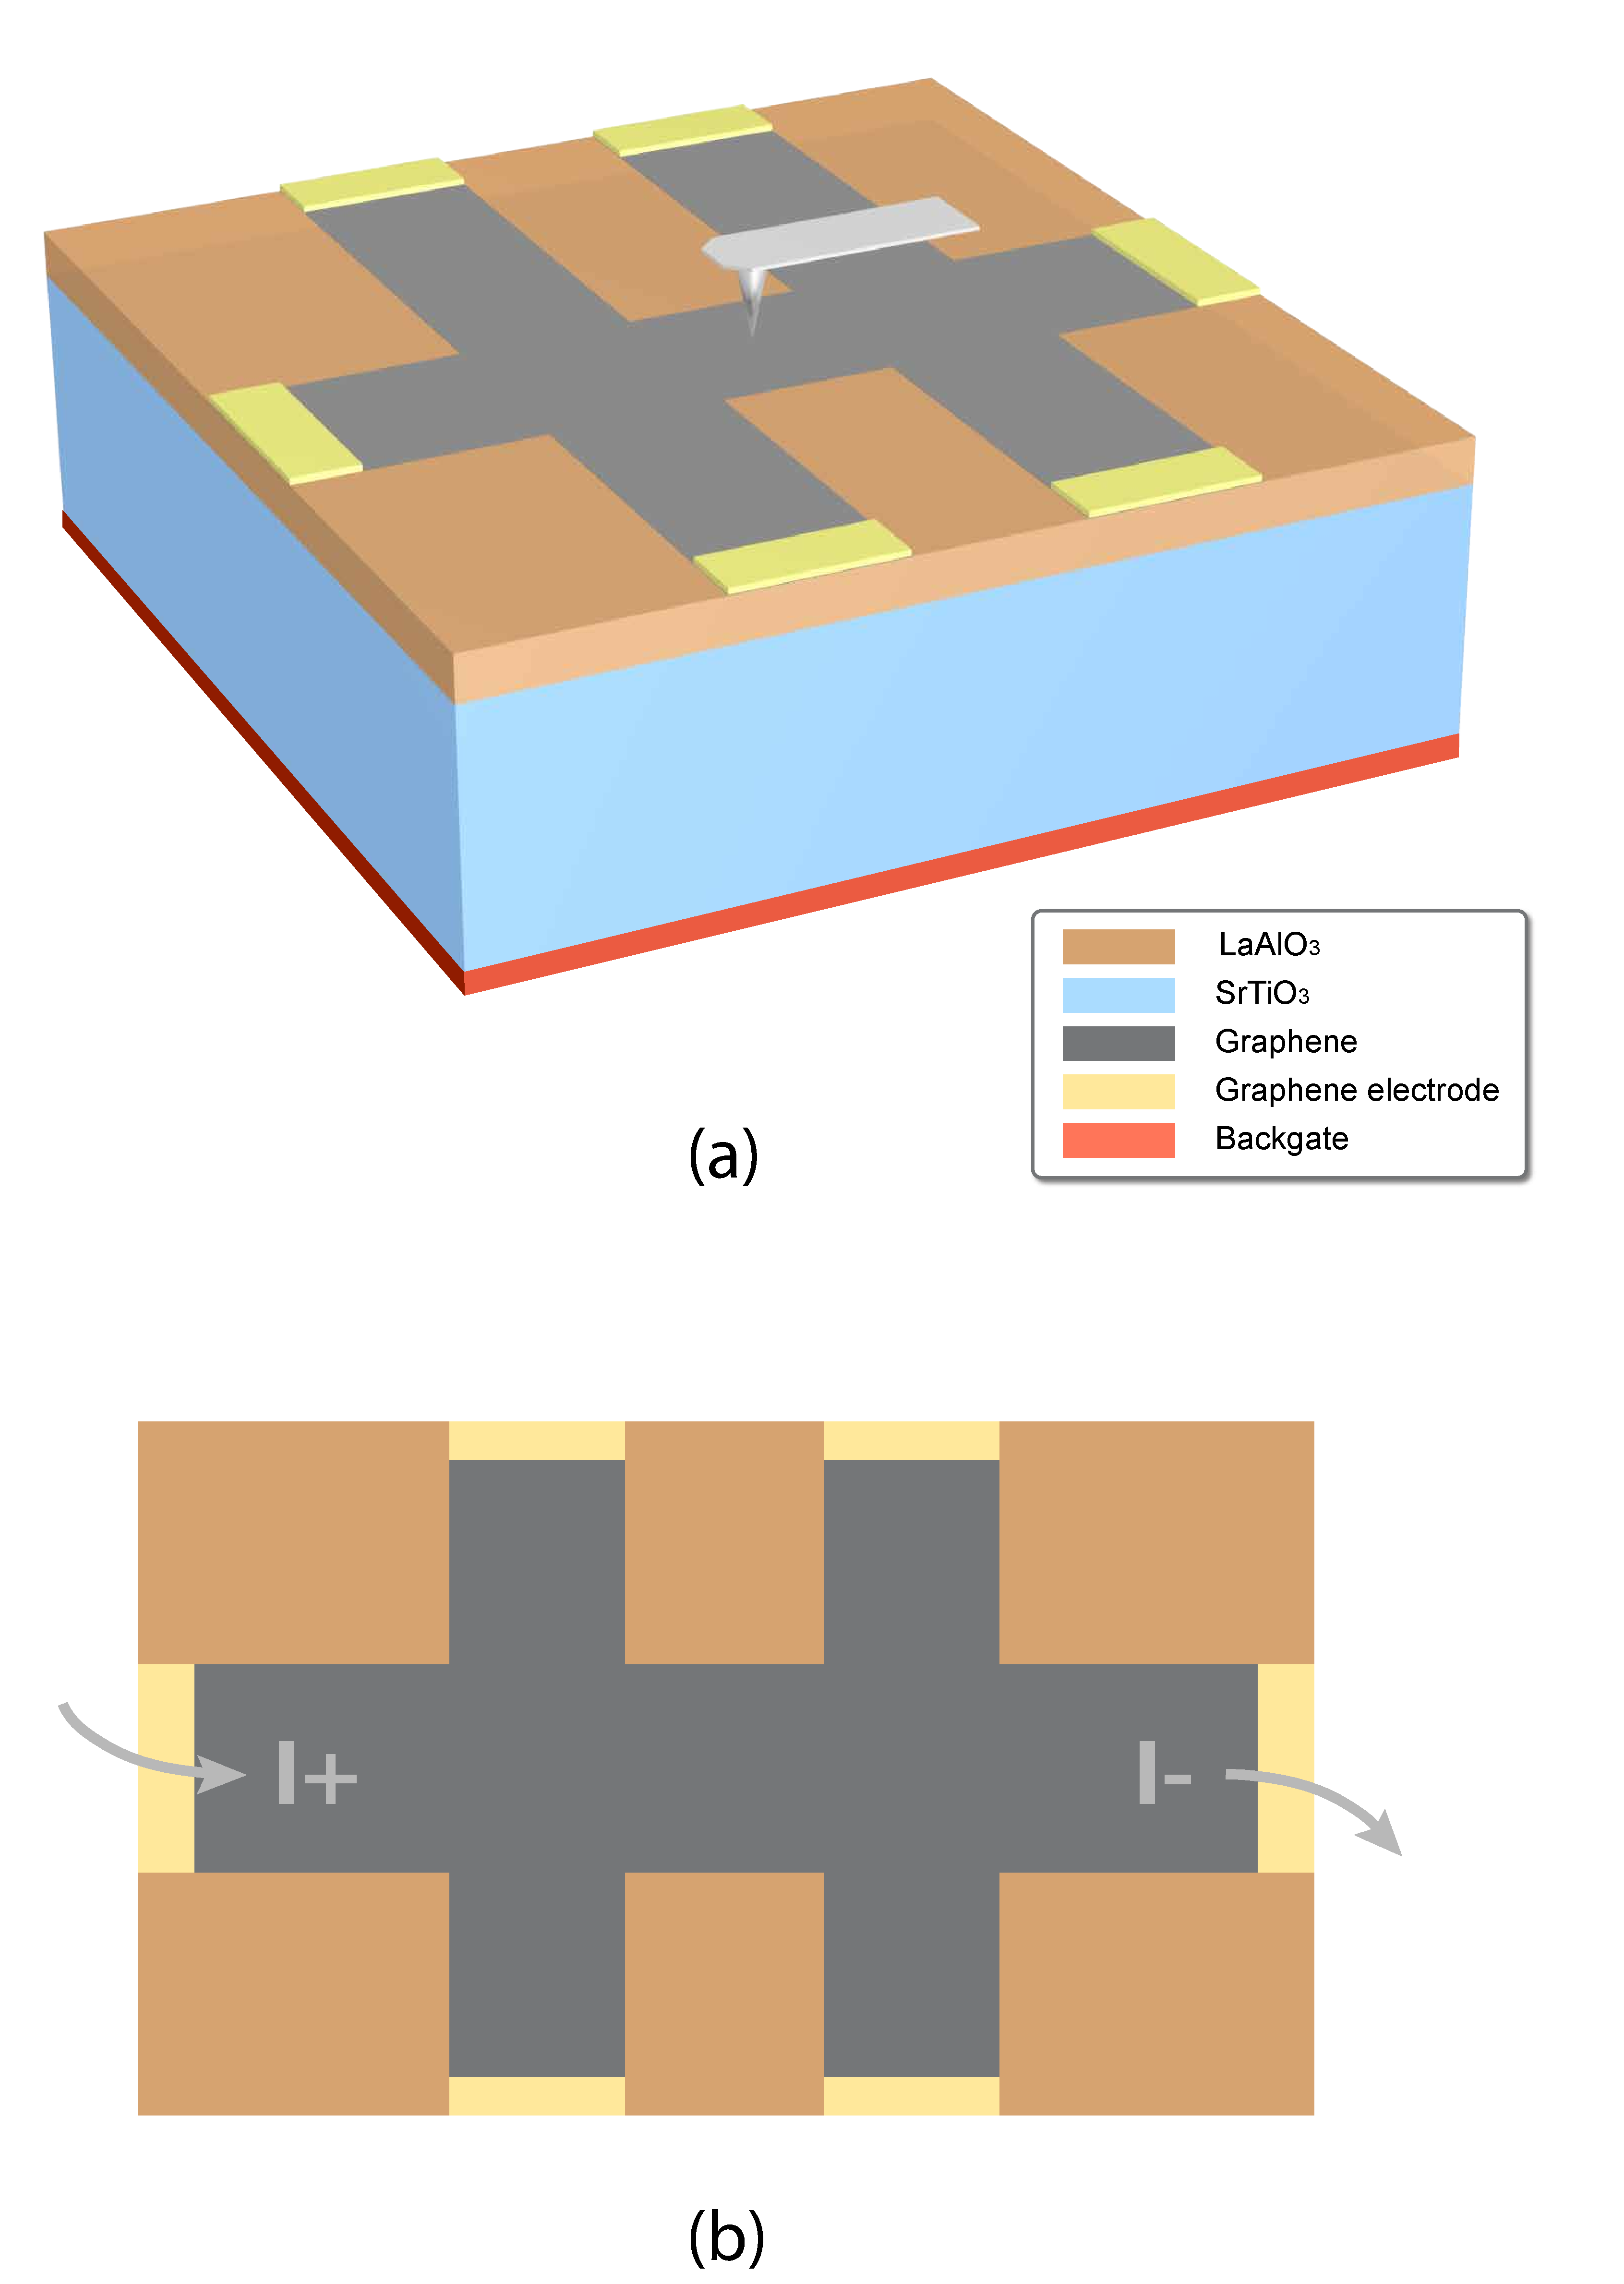
\includegraphics[width=.7\textwidth]{Drawing/HallDevice.pdf}
	\caption[Setup for graphene/LAO/STO device measurement]{Setup for graphene/LAO/STO device measurement. (a) The graphene on LAO/STO is patterned into Hall bar shape. The bottom of the LAO/STO is painted with silver epoxy for applying backgate gate voltages and control the chemical potential of graphene. A c-AFM tip is used to shift the local CNP of graphene. (b) A current flows through the graphene device, while the longitudinal and transverse voltages are measured.}
	\label{FIG:HallDevice}
\end{figure}

\subsection{Charge-neutrality point}

The tight binding model suggests that the density of state of graphene near the Dirac point is zero\cite{neto2009electronic}, as Figure \ref{FIG:DOS} shows. The resistance of graphene would have a maximum as the chemical potential gets close to the Dirac point. In Figure \ref{FIG:DiracPeak}, the resistance of graphene is measured as a function of the backgate voltage $V_\mathrm{bg}$, which is applied to the bottom of the sample. The thickness of the substrate is 5 mm. At T = 2 K, the dielectric constant of STO $\epsilon_r \sim 20,000$. Therefore, the gate voltage applied to the bottom of STO can effectively tune the chemical potential of graphene on the top surface. 

\begin{figure}[h!]
	\centering
	\vspace{0.85cm}
	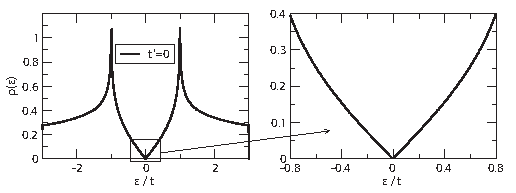
\includegraphics[width=.9\textwidth]{Drawing/DOS.pdf}
	\caption[The density of state of graphene near the Dirac point]{The density of state of graphene near the Dirac point, assuming the hopping energy between the second nearest neighbor $t'$ is zero. $\epsilon$ is the Fermi energy, $t$ is the hopping energy in the tight binding model. Adapted from \cite{neto2009electronic}.}
	\label{FIG:DOS}
\end{figure}

\begin{figure}[h!]
	\centering
	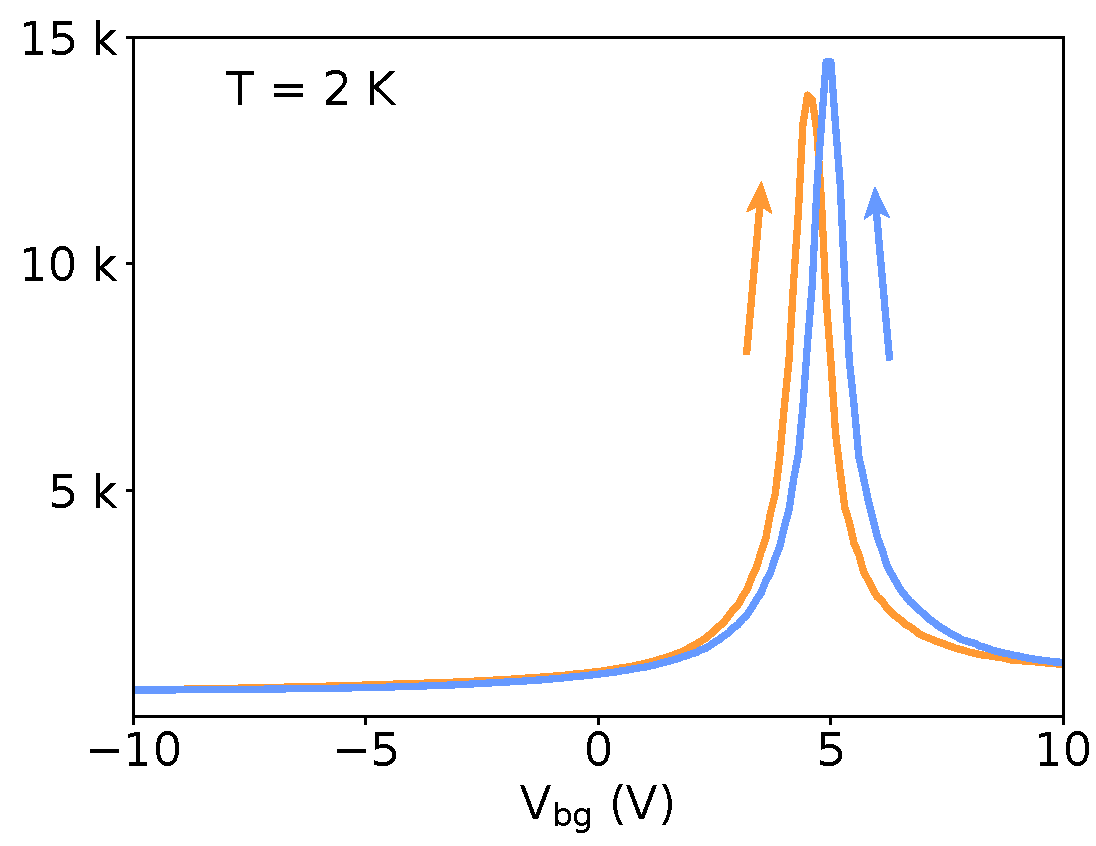
\includegraphics[width=.5\textwidth]{Drawing/DiracPeak.pdf}
	\caption[Graphene resistance as a function of backgate voltage]{Graphene resistance as a function of backgate voltage. The resistance shows a maximum when the chemical potential reaches the CNP. The positions of the CNP are different for the forward and backward sweeps. The arrows indicate the directions of sweeping. Measured at $T = 2$ K.}
	\label{FIG:DiracPeak}
\end{figure}

The effect of STO dielectric constant change as the temperature changes is critical for graphene devices on LAO/STO, as found in literatures\cite{couto2011transport}. Figure \ref{FIG:ResistanceTemp} demonstrates the change of resistance as a function of $V_\mathrm{bg}$. As the temperature drops, the dielectric constant of STO increases from 300 to 20,000, about two orders of magnitude. Therefore the effective gating range under the same backgate sweeping range ($-15$ V to $+15$ V in this figure) also drastically increases. 

Another effect of the LAO/STO substrate is the hysteresis behavior under backgate sweeping. The position of CNP on $V_\mathrm{bg}$ shifts after each backgate voltage sweep. Although STO is not ferroelectric material, the dipole moment induced by displacement of oxygen atoms would result in ferroelectric-like hysteresis behavior\cite{sachs2014ferroelectric}. Similar hysteretical behavior of graphene on LAO/STO has been reported elsewhere\cite{jnawali2017room}. 

\begin{figure}[h!]
	\centering
	\vspace{0.85cm}
	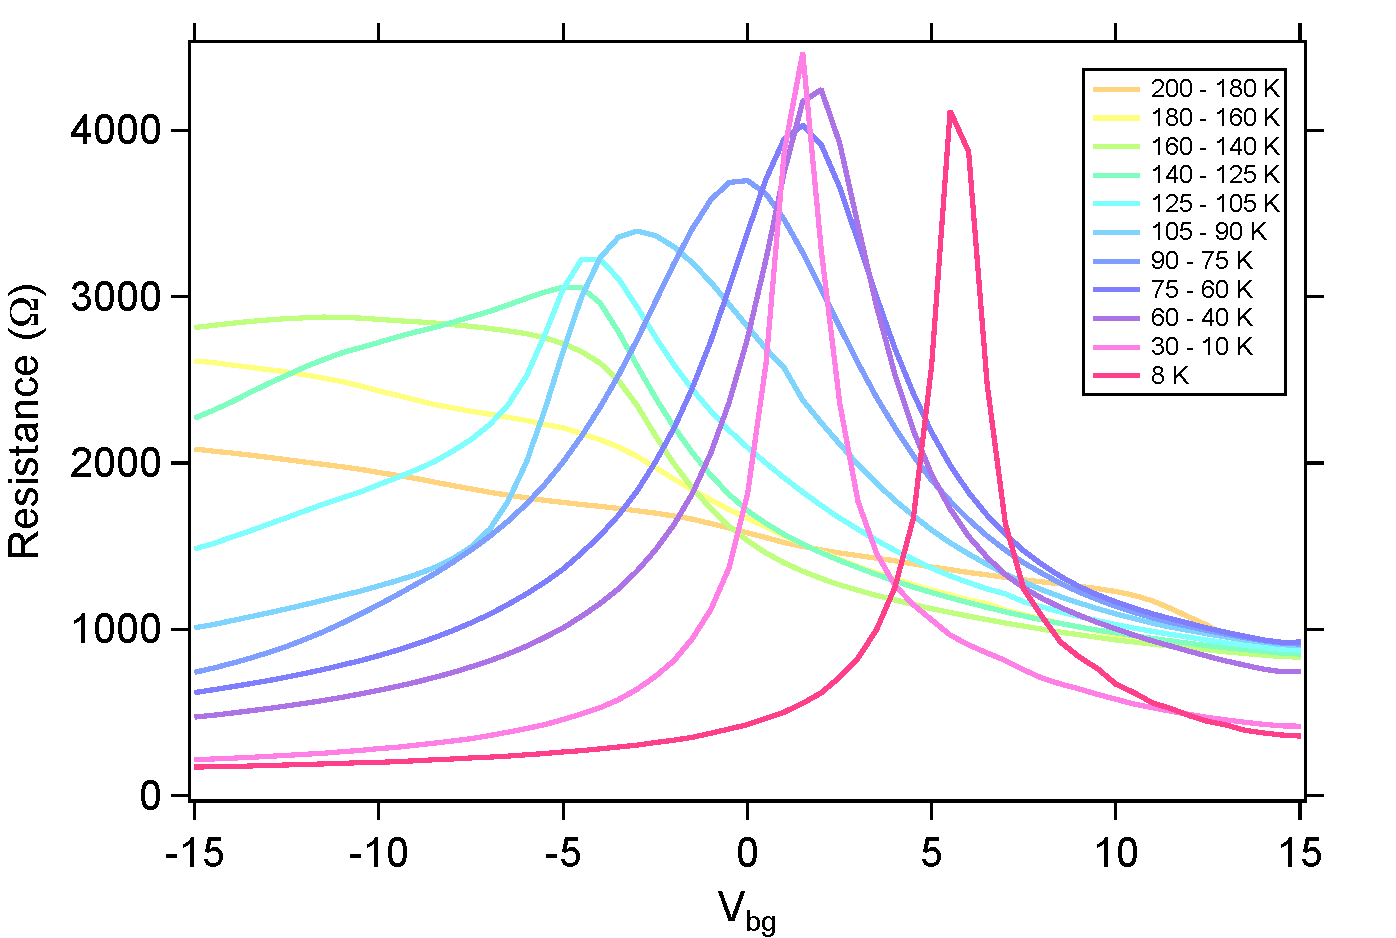
\includegraphics[width=.8\textwidth]{Drawing/ResistanceTemp.pdf}
	\caption[Resistance as a function of $V_\mathrm{bg}$ sweep at different temperatures]{Resistance as a function of $V_\mathrm{bg}$ sweep at different temperatures. The width of the CNP clearly shows the change of dielectric constant of STO as a function of temperature.}
	\label{FIG:ResistanceTemp}
\end{figure}

\subsection{Carrier densities and mobilities}
\label{SEC:CarrierDensityMobility}
\begin{figure}[h!]
	\centering
	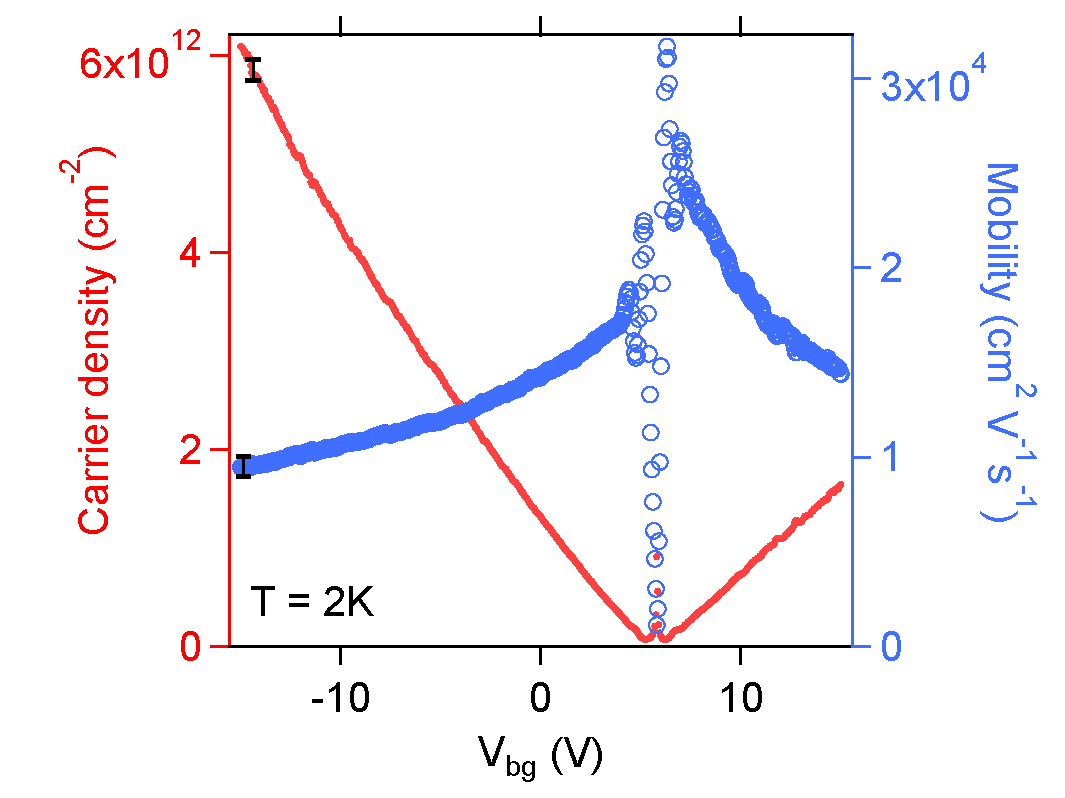
\includegraphics[width=.65\textwidth]{Drawing/CarrierDensityMobility.pdf}
	\caption[Carrier density and mobility of graphene measured from Hall effect]{Carrier density and mobility of graphene measured from Hall effect. The high dielectric constant makes it possible for the backgate to tune the graphene to a high carrier density on the hole side. However, the tuning effect saturates on the electron side due to the shielding of 2DEG induced on the interface. The carrier density is not well defined close to the CNP, due to the existence of electron-hole puddles. The quality of graphene is higher than most of the CVD graphene transferred on SiO$_2$, and the mobility can reach 30,000 cm$^2$V$^{-1}$s$^{-1}$. The error bars on the curves indicate the 95\% confidence intervals of the carrier density and mobility.}
	\label{FIG:CarrierDensityMobility}
\end{figure}

The carrier density and mobility of graphene can be measured from the Hall effect, using equation \ref{EQN:Hall}. From Figure \ref{FIG:CarrierDensityMobility} it can be seen that the high dielectric constant of STO at low temperature enables graphene gating to up to $1 \times 10^{13}$ $\mathrm{cm}^{-2}$ on the hole side (not shown in the Figure). On the electron side, due to the 2DEG electron gas induced by the high backgate voltage, the gating effect on graphene is shielded, and the carrier density usually saturates at about $n = 1 \times 10^{12}$ $\mathrm{cm}^{-2}$. Close to the CNP the carrier density and mobility are not well defined due to the existence of electron-hole puddles. The Hyflon transfer method followed by contact AFM cleaning leaves the graphene on LAO/STO with high quality. The mobility of graphene reach $30,000$ cm$^{2}$V$^{-1}$s$^{-1}$, higher than most of the graphene on SiO$_2$ substrates\cite{li2016method, li2018high}. 

\subsection{Quantum Hall effect}

As discussed in Section \ref{SEC:QuantumHall}, single layer graphene has unique half-integer filling factors with degeneracy $N = 4$ from spin and valley pseudo-spin. The Hall conductance is
$$
\sigma_{xy} = \pm 4\left(n + \frac{1}{2}\right)\frac{e^2}{h}
$$
in quantum Hall regime. The longitudinal resistance is suppressed except when the Fermi energy is transiting between Landau levels, and the localized states start to be filled. Figure \ref{FIG:HallResistance} demonstrate the longitudinal and transverse resistance of graphene device in a magnetic field of $B = 5$ T. The blue line is the Hall resistance that shows quantum Hall effect plateaus, with the filling factor $\nu$ marked by the numbers. The red line is the longitudinal resistance showing non-zero resistance at the transition energy between Landau levels.

\begin{figure}[h!]
	\centering
	\includegraphics[width=.55\textwidth]{Drawing/HallResistance.pdf}
	\caption[Integer quantum Hall effect of single-layer graphene]{Integer quantum Hall effect of single-layer graphene. The plateaus in the transverse resistance (blue line) are clearly visible.}
	\label{FIG:HallResistance}
\end{figure}

\section{Graphene p-n junction edge-state engineering}
\label{SEC:PNJunction}

In this section, the experiment of using c-AFM to dope the graphene into $p$-$n$ junction to reversibly engineer the edge state mixing is discussed. The measurements were performed at $T = 2$ K. 

\subsection{1D waveguide and quantum Hall edge channels}

In semi-classical point of view, the electrons under high magnetic field would cycle in the 2DEG and bounce back from the edges or scattering centers. If the scattering center is far from the edge, the electrons would cycle around the scattering centers and be trapped in the localized state. If the scattering centers are close to the edge, the electrons would then collide with the edge and keep moving in the same direction. Therefore, chiral edge channels are formed with backscattering being suppressed. The transport of the edge state in the quantum Hall regime can be quantified with Landauer-B{\"u}ttiker formalism for 1D waveguides\cite{buttiker1986four, buttiker1988absence}.

\begin{figure}[h!]
	\centering
	\vspace{0.85cm}
	\includegraphics[width=.5\textwidth]{Drawing/Channel.pdf}
	\caption[A conductor channel connecting two reservoirs]{A conductor channel connecting two reservoirs. The chemical potential of the two reservoirs are $\mu_1$ and $\mu_2$. The shaded region introduces elastic scatterings.}
	\label{FIG:Channel}
\end{figure}

Consider a strip on $x$-$y$ plane, as shown in Figure \ref{FIG:Channel}. The Hamiltonian is
$$
H = \frac{1}{2m}\left(p_x^2 + p_y^2\right) + V(y)
$$ 
$x$ is along the direction of the strip and $y$ is transverse to the strip. The wavefunction can be separated into the form
$$
\psi_{j, k}(x, y) = e^{ikx} f_j(y),
$$
$k$ is the wave vector along the $x$ direction, and $f_j(y)$ is the eigenfunction in $y$ direction with energy $E_j$. The Fermi energy is 
$$
E_F = E_j + \frac{\hbar^2 k_j^2}{2m}
$$
which is the sum of longitudinal and transverse energies, with 2$N$ state, where $N$ is the number of transverse energy levels $E_j$ below $E_F$. $\mu_1$ and $\mu_2$ are the chemical potentials of the two reservoirs, with $\mu_1 > \mu_2$. Only energy between $\mu_1$ and $\mu_2$ contribute to the current flowing from left to right. The current in channel $j$ is 
$$
I_j = \frac{dn}{dE_j}ev_j\Delta\mu,
$$
with 
$$
v_j = \frac{1}{\hbar}\frac{dE_j}{dk}, \ \ \ \Delta \mu = \mu_1 - \mu_2
$$
and $v_j$ being the velocity along channel $j$. In one dimension, density of state is
$$
\frac{dn}{dk} = \frac{1}{2\pi},
$$
and therefore the current in channel $j$ is
$$
I_j = \frac{e}{h}\Delta\mu.
$$
The current for all $N$ channels is the sum of currents in individual channels
$$I = N\frac{e}{h}\Delta\mu.$$
Using the voltage drop $\Delta \mu = eV$ and Ohm's law, the resistance of the conductor with $N$ channels is
$$
R = \frac{h}{e^2}\frac{1}{N}
$$ 
which is quantized. Consider there elastic scattering that redistributes energies between the $N$ channels, the resistance becomes\cite{buttiker1988absence}
$$
R = \frac{h}{e^2}\frac{1}{T}
$$
$T = \sum_{i,j=1\ldots N} T_{ij}$, and $T_{ij}$ is the transmission probability from channel $j$ into channel $i$. 

\subsection{Edge channel mixing of graphene unipolar/bipolar junction in quantum Hall regime}

In the quantum Hall regime, edge channels of graphene can be described by the Landauer-B{\"u}ttiker formalism. When two adjacent regions of graphene have different carrier density and Landau level filling factors in the magnetic field, the numbers or directions of channels will be different which would cause channel mixing. In Figure \ref{FIG:Mixing}(a), the two adjacent regions have different carrier densities, and therefore the filling factors and the number of edge channels for the two areas are different. The edge currents flow in the same direction (unipolar), but part of the current would be reflected into the interface of the two regions. In Figure \ref{FIG:Mixing}(b), the two areas have the opposite carrier types, and the directions of edge currents are opposite (bipolar). The edge channels would mix on the interface. In both cases, the longitudinal resistance is non-trivial as a result of channel mixing.

\begin{figure}[h!]
	\centering
	\vspace{0.85cm}
	\includegraphics[width=.4\textwidth]{Drawing/Mixing.pdf}
	\caption[Unipolar and bipolar junctions]{Unipolar and bipolar junctions. (a) Two regions with the same carrier type but the region on the left-hand side has more edge channels than the right-hand side. The currents are flowing in the same directions, and part of the current would be reflected on the interface of the two regions. (b) Two regions with different carrier types. The currents flow in opposite directions in the two regions, and would mix on the interface of the two regions.}
	\label{FIG:Mixing}
\end{figure}

\subsubsection{Unipolar junction}

\begin{figure}[h!]
	\centering
	\includegraphics[width=.7\textwidth]{Drawing/Unipolar.pdf}
	\caption[Edge currents of the unipolar junction]{Edge currents of the unipolar junction. Assume $\mu_L > \mu_R$ and the current is flowing towards right. All the voltage leads have zero net currents. Adapted from \cite{li2019reconfigurable}.}
	\label{FIG:Unipolar}
\end{figure}

For the unipolar case, as shown in Figure \ref{FIG:Unipolar}, assume the current is sourced from the left and $\mu_L > \mu_R$. Filling factors $|\nu_1| > |\nu_2|$ and the currents are flowing clock-wise (same as Figure \ref{FIG:Mixing}(a)). The chemical potential of the four voltage leads are $\mu_A$, $\mu_B$, $\mu_C$ and $\mu_D$. $I_1$ to $I_8$ are the currents flowing between the current and voltage leads:
\begin{equation}
\label{EQN:MixCurr1}
\begin{split}
I_1 & = \frac{e}{h}\mu_L|\nu_1|, \ \ \ \  I_2 = \frac{e}{h}\mu_A|\nu_1|, \\
I_3 & = I_2 - I_M, \ \ \ \ I_4 = \frac{e}{h}\mu_B|\nu_2| \\
I_5 & = \frac{e}{h}\mu_C|\nu_1|, \ \ \ \ I_6 = I_M + I_7 \\
I_7 & = \frac{e}{h}\mu_D|\nu_2|, \ \ \ \ I_8 = \frac{e}{h}\mu_R|\nu_2|
\end{split}
\end{equation}

The region on the left hand side has more channels, and therefore the excessive current is reflected into the interface and $I_M = \frac{e}{h}\mu_L(|\nu_1|-|\nu_2|)$. The net currents flowing into and out of the four voltages leads are zero, i.e.
$$
I_1 = I_2, \ \ I_3 = I_4, \ \ I_5 = I_6, \ \ I_7 = I_8
$$
and therefore the chemical potentials of the four leads are
\begin{equation}
\label{EQN:MixMu1}
\mu_A = \mu_B = \mu_L, \ \ \mu_C = \mu_L + \frac{|\nu_2|}{|\nu_1|}(\mu_L - \mu_R), \ \ \mu_D = \mu_R.
\end{equation}
From equation \ref{EQN:MixCurr1} and \ref{EQN:MixMu1}, the total current from left to right is 
$$
I = I_1 - I_5 = \frac{e}{h}(\mu_L - \mu_R)|\nu_1|,
$$ 
and the longitudinal resistances are 
\begin{equation}
\label{EQN:Mixing1}
\begin{split}
R_{AB} & = \frac{\mu_A - \mu_B}{eI} = 0, \\
R_{CD} & = \frac{\mu_C - \mu_D}{eI} = \frac{h}{e^2}\left(\frac{1}{|\nu_2|} - \frac{1}{|\nu_1|}\right).
\end{split}
\end{equation}

\subsubsection{Bipolar junction}

\begin{figure}[h!]
	\centering
	\includegraphics[width=.7\textwidth]{Drawing/Bipolar.pdf}
	\caption[Edge currents of the bipolar junction]{Edge currents of the bipolar junction. Assume $\mu_L > \mu_R$ and the current is flowing towards right. All the voltage leads have zero net currents. Adapted from \cite{li2019reconfigurable}.}
	\label{FIG:Bipolar}
\end{figure}

For the bipolar case, as shown in Figure \ref{FIG:Bipolar}, again assume that the chemical potentials $\mu_L > \mu_R$. The two regions have different carrier type and the currents are flowing in the opposite directions. The channels are mixed at the interface, and therefore $I_M$ is equal to the sum of currents from each side, and then redistributed into edge channels on the bottom. Therefore the edge currents are
\begin{equation}
\label{EQN:MixCurr2}
\begin{split}
I_1 = \frac{e}{h}\mu_L|\nu_1|, & \ \ \ \   I_2 = \frac{e}{h}\mu_A|\nu_1|, \\
I_3 = \frac{e}{h}\mu_B|\nu_2|, & \ \ \ \ I_4 = \frac{e}{h}\mu_R|\nu_2| \\
I_5 = \frac{e}{h}\mu_C|\nu_1|, & \ \ \ \  I_6 = \frac{|\nu_1|}{|\nu_1|+|\nu_2|} \cdot I_M \\
I_7 = \frac{|\nu_2|}{|\nu_1|+|\nu_2|} \cdot I_M, & \ \ \ \ I_8 = \frac{e}{h}\mu_D|\nu_2|,
\end{split}
\end{equation}
with $I_M = I_2 + I_3$. The net currents flowing into and out of the four voltages leads are zero, i.e.
$$
I_1 = I_2, \ \ I_3 = I_4, \ \ I_5 = I_6, \ \ I_7 = I_8
$$
and therefore the chemical potentials of the four leads are
\begin{equation}
\label{EQN:MixMu2}
\mu_A = \mu_L, \ \ \mu_B = \mu_R, \ \ \mu_C = \mu_D = \frac{\mu_L|\nu_1| + \mu_R|\nu_2|}{|\nu_1| + |\nu_2|}.
\end{equation}
From equation \ref{EQN:MixCurr2} and \ref{EQN:MixMu2}, the total current from left to right is 
$$
I = I_1 - I_5 = \frac{e}{h} \cdot \frac{|\nu_1||\nu_2|}{|\nu_1| + |\nu_2|} \cdot (\mu_L - \mu_R),
$$ 
and the longitudinal resistances are 
\begin{equation}
\label{EQN:Mixing2}
\begin{split}
R_{AB} & = \frac{\mu_A - \mu_B}{eI} = \frac{h}{e^2}\left(\frac{1}{|\nu_1|} + \frac{1}{|\nu_2|}\right), \\
R_{CD} & = \frac{\mu_C - \mu_D}{eI} = 0.
\end{split}
\end{equation}

\subsection{Graphene doping using c-AFM}

There have been efforts to locally control the CNP of graphene on silicon or hBN substrates using AFM\cite{schmidt2013mixing} or STM\cite{velasco2016nanoscale}. However, those doping techniques are either non-reversible or can only be performed in ultra-high vacuum and low temperature, which limits the applications. In this research, it is found that the metal-insulator transition in LAO/STO can be used to reversibly pattern interacting edge channels in a proximal graphene layer under ambient conditions. The tip can locally shift the CNP of graphene with a positive bias voltage. Therefore, c-AFM writing can be used to selectively dope graphene regions and engineer edge state mixing in quantum Hall regime.

The mechanism of using c-AFM to shift the CNP locally is similar to c-AFM nanostructure lithography technique discussed in section \ref{SEC:AFMLitho}. As Figure \ref{FIG:GrapheneAFM} shows, when a positively biased tip scans the graphene in contact mode while the graphene is grounded, a trace of protons will be left on graphene, and permeate\cite{hu2014proton} to the interface between graphene and LAO. The proton would locally dope the graphene and shift the CNP. 

\begin{figure}[h!]
	\centering
	\vspace{0.85cm}
	\includegraphics[width=.45\textwidth]{Drawing/GrapheneAFM.pdf}
	\caption[Graphene doping using c-AFM writing technique]{Graphene doping using c-AFM writing technique. A trace of protons would be left by the tip and permeate to the interface of graphene and LAO. The voltage of the back gate is kept at zero during c-AFM writing.}
	\label{FIG:GrapheneAFM}
\end{figure}

One standard method of monitoring the doping level of graphene is to sweep the back-gate voltage and compare the position of CNP before and after the doping. The method cannot be used for graphene on LAO/STO substrates for two reasons: (1) the surface of LAO is not charge neutral, and therefore the CNP is not at $V_\mathrm{bg}$ is not at 0 V even without c-AFM doping; (2) the $V_\mathrm{bg}$ is subject to significant hysteresis\cite{couto2011transport, jnawali2017room} (also shown in Figure \ref{FIG:DiracPeak}) and thus is not a reliable indicator of doping level with respect to CNP. Instead, the four-terminal resistance of graphene is measured \emph{in situ} to monitor the doping level change during the c-AFM writing process. 

In Figure \ref{FIG:WritingResistance}, a graphene device is scanned with c-AFM with a bias voltage of $V_\mathrm{tip} = +17$ V continuously. The scanned region covers the entire device, as shown in the inset of the figure. The current flows from left to right, and the longitudinal resistance is measured as a function of time as the scanning proceeds. At $t$ = 0 s, the graphene is $n$-type doped. The AFM scanning speed is 10 $\mu$m/s, and it takes 260 s to scan the graphene device (5 $\mu$m $\times$ 10 $\mu$m). Fifteen consecutive scans are recorded. Blue dots mark the beginning/ending of the consecutive AFM raster scans. The positive charges left by the tip increase the local doping level and drives the chemical potential further into the $n$-type region (illustrated by the Dirac cone in the inset). Within each scan, the resistance decreases at the beginning due to the doping, and then start to recover when the scan is half finished. The green region marks one complete scan. The resistance recovery speed is observed to be related to the environmental humidity and is possibly caused by the recombination of protons with water molecules in the air. The terminal resistance after each scan (marked by the blue dots) decreases as the scan proceeds, indicating that the $n$-type doping level of graphene is increasing as the scan proceeds.

\begin{figure}[h!]
	\centering
	\includegraphics[width=1\textwidth]{Drawing/WritingResistance.pdf}
	\caption[Monitoring the doping level change during the c-AFM writing process]{Monitoring the doping level change during the c-AFM writing process. The rectangle in the inset is scanned with c-AFM tip continuously, while the four-terminal resistance is measured \textit{in situ}. The blue dots mark the beginning/ending of the consecutive scans. The green region marks one complete scan. The resistance drops in the first half of each scan, and then recovers as the scan proceeds. The terminal resistance of each scan decreases as the scan proceeds, indicating increasing $n$-type doping level of graphene. Adapted from \cite{li2019reconfigurable}.}
	\label{FIG:WritingResistance}
\end{figure}

The graphene doping from the positively biased c-AFM tip is reversible. After the c-AFM writing and the change in four-terminal resistance being observed, a scan with $V_\mathrm{tip}= -5$ V on the c-AFM tip will partially remove the previous writing effect. Scans with negative $V_\mathrm{tip}$ need to be carefully conducted, and the c-AFM tip should be connected in series with a 1 G$\Omega$ resistor, since graphene can be oxidized as anode\cite{alaboson2011conductive, byun2011nanoscale}. Also, graphene has to be detached from groundings to avoid oxidation damages\cite{alaboson2011conductive}. Using the c-AFM writing method the graphene can be locally doped reversibly and various devices can be created on graphene/LAO/STO heterostructure\cite{li2019reconfigurable, guo2018reconfigurable, li2019reversible, guo2019coulomb}. 

\subsection{Measurement of graphene edge state mixing}

The edge state mixing engineering can be achieved by doping graphene regions with the c-AFM writing technique. In Figure \ref{FIG:GrapheneDopedHall}, the right-hand-side region of the graphene device is written with c-AFM tip and locally doped with positive charges. Carrier densities measured on the two pairs of Hall electrodes (Hall A and Hall B) indicate that the CNP for the written area (B) is shifted to the left.

\begin{figure}[h!]
	\centering
	\includegraphics[width=.7\textwidth]{Drawing/GrapheneDopedHall.pdf}
	\caption[Carrier density of locally doped graphene]{Carrier density of locally doped graphene. Carrier densities of the two pairs of Hall electrodes (Hall A and Hall B) are measured at $T = 2$ K. The CNP of the written region (B) is shifted to the left, indicating the doping effect of c-AFM writing. Adapted from \cite{li2019reconfigurable}.}
	\label{FIG:GrapheneDopedHall}	
\end{figure}

The longitudinal resistance (as shown in the inset of Figure \ref{FIG:GrapheneDopedHall}) is also measured as a function of $V_\mathrm{bg}$ to indicate the effect of c-AFM writing. Figure \ref{FIG:DiracPointSplit}(a) is the resistance measured before c-AFM writing, and a single Dirac peak can be seen. Figure \ref{FIG:DiracPointSplit}(b) is measured after the writing, and a second Dirac peak is distinguishable. The peak on the left-hand side corresponds to the written area (B in the inset of Figure \ref{FIG:GrapheneDopedHall}).

\begin{figure}[h!]
	\centering
	\includegraphics[width=.75\textwidth]{Drawing/DiracPointSplit.pdf}
	\caption[Longitudinal resistance as a function as $V_\mathrm{bg}$]{Longitudinal resistance as a function as $V_\mathrm{bg}$. (a) is measured before c-AFM writing as a control measurement. Dirac peak is clearly visible. (b) is measured after c-AFM writing. Splitting of Dirac peak can be observed. The peak on the left hand side is correspond to the written area (shown in the inset of Figure \ref{FIG:GrapheneDopedHall}). Adapted from \cite{li2019reconfigurable}.}
	\label{FIG:DiracPointSplit}
\end{figure}

Graphene sample with half of the device written by c-AFM is then measured in magnetic field with $B = 7$ T. The longitudinal resistances are measured from the bottom ($R_\mathrm{xx1}$) and top ($R_\mathrm{xx2}$) pairs of electrodes as functions of $V_\mathrm{bg}$. The result is shown in Figure \ref{FIG:EdgeChannels}(a). $R_\mathrm{xx1}$ is quantized at $h/3e^2$ at around $V_\mathrm{bg} = 0$ V, then is suppressed between 1 V and 3 V, and quantized at $h/3e^2$ again around $V_\mathrm{bg} = 5$ V. $R_\mathrm{xx2}$ is suppressed around $V_\mathrm{bg} = 0$ V and 5 V, and is quantized at $h/e^2$. 

\begin{figure}[p]
	\centering
	\includegraphics[width=1.0\textwidth]{Drawing/EdgeChannels.pdf}
	\caption[The edge channel mixing changes as $V_\mathrm{bg}$ is swept from $-10$ V to $+10$ V]{The edge channel mixing changes as $V_\mathrm{bg}$ is swept from $-10$ V to $+10$ V. (a) $R_\mathrm{xx1}$ and $R_\mathrm{xx2}$ are quantized at values predicted by equation \ref{EQN:Mixing1} and \ref{EQN:Mixing2}. (b) Zoomed-in plot of Figure \ref{FIG:GrapheneDopedHall}. (c) Filling factors and edge current directions of the three cases of edge state mixing. Adapted from \cite{li2019reconfigurable}.}
	\label{FIG:EdgeChannels}
\end{figure}

Figure \ref{FIG:EdgeChannels}(b) is the zoomed-in plot of Figure \ref{FIG:GrapheneDopedHall} around the CNP. At line cut (I), both regions are $p$-type doped, as shown in the left sub-figure of (c). However, the two regions have different Landau level filling factors in the magnetic field, and therefore the number of edge channels are different. The excessive currents from the left-hand-side region are reflected into the interface in the middle and then mixed with the currents from the right on the bottom. The channel mixing result in non-trivial resistance values in $R_\mathrm{xx1}$ and $R_\mathrm{xx2}$ that can be predicted with equation \ref{EQN:Mixing1}. At line cut (III), both regions are $n$-type doped, but again different filling factors and number of edge channels in the magnetic field. The longitudinal resistances can also be calculated using the same formalism. At line cut (II), the two regions have opposite carrier types, and the currents are flowing different directions and mixed on the interface in the middle (shown by the arrows in the middle sub-figure of \ref{FIG:GrapheneDopedHall}(c)). The quantized resistances can be calculated from equation \ref{EQN:Mixing2}.


\begin{figure}[h!]
	\centering
	\includegraphics[width=0.90\textwidth]{Drawing/MixingIntensityPlot.pdf}
	\caption[Intensity plot of longitudinal resistances]{Intensity plot of longitudinal resistance $R_\mathrm{xx1}$ (a) and $R_\mathrm{xx2}$ (b) as functions of $V_\mathrm{bg}$ and magnetic field sweep. The values of $R_\mathrm{xx1}$ and $R_\mathrm{xx2}$ are swapped when the direction of magnetic field is reversed. Adapted from \cite{li2019reconfigurable}.}
	\label{FIG:MixingIntensityPlot}
\end{figure}

When the magnetic field is reversed, the directions of current in all three cases are reversed. Therefore the values of $R_\mathrm{xx1}$ and $R_\mathrm{xx2}$ are swapped. To demonstrate the transition of longitudinal resistances when the direction of magnetic field is flipped, $R_\mathrm{xx1}$ and $R_\mathrm{xx2}$ are measured at magnetic fields from $-7$ T to $+7$ T, while $V_\mathrm{bg}$ is swept at each magnetic field step. Figure \ref{FIG:MixingIntensityPlot} is the intensity plot of $R_\mathrm{xx1}$ and $R_\mathrm{xx2}$ as functions of $V_\mathrm{bg}$ and $B$. In Figure \ref{FIG:MixingIntensityPlot}(a) $R_\mathrm{xx1}$ is clearly quantized at $h/3e^2 \approx 8.6 \ \mathrm{k}\Omega$ at $B = +7$ T. The quantization gradually disappears as $B$ gets close to 0. Then $R_\mathrm{xx1}$ start to be quantized at $h/e^2 \approx 25.8 \ \mathrm{k}\Omega$ when the field increases in the opposite direction. In Figure \ref{FIG:MixingIntensityPlot}(b) $R_\mathrm{xx1}$ shows the opposite behavior as the field is stepped from $-7$ T to $+7$ T. The observation of mixed edge channel is consistent with results reported elsewhere\cite{williams2007quantum, lohmann2009four, amet2014selective, abanin2007quantized, ki2010dependence, klimov2015edge, woszczyna2011graphene, ozyilmaz2007electronic, schmidt2013mixing} and is the direct proof of doping effect of c-AFM writing on graphene with a LAO/STO substrate. The fact that the result of mixing follows the Landauer-B{\"u}ttiker formalism also indicates that the transport in graphene is not affected by the 2DEG in the LAO/STO at $T = 2$ K.

\section{Graphene band-structure engineering with superlattice}

Superlattice has been proven to be a useful technique for band-structure engineering in semiconductors systems\cite{tsu2010superlattice}. Early theoretical works have predicted that graphene with potential superlattice potential could have strong Fermi energy renormalization that leads to anisotropic transport\cite{park2008anisotropic} and supercollimation of electron beams\cite{park2008electron}. Superlattice in graphene would also lead to a new generation of Dirac points near each valley\cite{park2008new}. An inherent advantage of 2D materials such as graphene is that the chemical potential can be tuned with electric-field effect, without introducing extra disorder\cite{cao2018correlated}. Experimentally, superlattice in graphene has been achieved in two methods: (1) direct electrical gating or etching using lithography\cite{dubey2013tunable, forsythe2018band, jessen2019lithographic}; (2) moir{\'e} pattern between graphene and substrates\cite{dean2013hofstadter, hunt2013massive, ponomarenko2013cloing} or two graphene layers with a twisted angle\cite{cao2016superlattice, cao2018correlated, cao2018unconventional, chen2018gate, yankowitz2018dynamic}. 

The moir{\'e} pattern (Figure \ref{FIG:Moire}) can generate superlattice with periodicity with a length scale orders of magnitude higher than the graphene crystal lattice and generate the ``Hofstadter butterfly'', induced by fractal miniband structures in strong magnetic field\cite{dean2013hofstadter, hunt2013massive, ponomarenko2013cloing}. It has also been predicted\cite{bistritzer2011moire} that the Fermi velocity at Dirac points becomes zero when the twisting angle of bi-layer graphene is equal to ``magic angles''. Theoretical work\cite{bistritzer2011moire, suarez2010flat, lopes2012continuum} further predicts that moir{\'e} patterns from twisted bi-layer graphene can modulate the interlayer hybridization and tailor flat-bands with a high density of states, which would enhance strong correlations between electrons and lead to more exotic phase such as Mott insulator\cite{cao2016superlattice, cao2018correlated, chen2018gate} or superconductivity\cite{cao2018unconventional}.

\begin{figure}[h!]
	\centering
	\includegraphics[width=0.8\textwidth]{Drawing/Moire.pdf}
	\caption[Moir{\'e} pattern]{Moir{\'e} pattern generated from two layers of honeycomb lattice with angular mismatch. The lattice constant can be an order of magnitude greater than the crystal lattice constant, depending on the mismatch angle.}
	\label{FIG:Moire}
\end{figure}

Superlattice from electrical gating\cite{forsythe2018band} or etching\cite{jessen2019lithographic} has more flexibility for the choosing patterns and lattice constants. Replica of Dirac cones and fractal Hofstadter spectra are also observed in graphene under electric potential superlattice from dielectric patterning\cite{forsythe2018band}. The direct patterning method involves e-beam lithography and is challenging when the lattice constant is smaller than 40 nm.

The c-AFM writing technique provides a method to reversibly pattern superlattice on graphene. The minimum feature size of c-AFM writing can reach $10-20$ nm\cite{huang2015electric}, and the superlattice generated from this technique is also more flexible compared to the graphene moir{\'e} pattern. The pattern written by c-AFM on graphene/LAO/STO heterostructure can also induce carrier density change on the LAO/STO interface\cite{huang2015electric}, therefore the superlattice potential is also tunable with a gate voltage applied to the interface. The interface properties such as electron pairing\cite{cheng2015electron}, superconductivity\cite{reyren2007superconducting}, spin-orbit coupling\cite{caviglia2010tunable, zhong2013theory} and magnetism\cite{bi2014room} of LAO/STO can lead to more complex interaction with the proximal graphene.

\subsection{Hofstadter spectra of superlattice}

\begin{figure}[h!]
	\centering
	\includegraphics[width=1.0\textwidth]{Drawing/HofstadterLandau.pdf}
	\caption[Landau levels and Hofstadter spectra]{Landau levels and Hofstadter spectra. (a) Magnetic flux through the electron orbits in magnetic field is quantized. (b) Landau fan diagram of the energy gaps in 2D system. (c) Additional Landau fans emerge under the periodic potential. The energy gaps can be described by equation \ref{EQN:Wannier}.}
	\label{FIG:HofstadterLandau}
\end{figure}

In the semi-classic view of Landau levels, the magnetic flux through the electron orbital is quantized (Figure \ref{FIG:HofstadterLandau}(a)). The number of states per area is given by $B/\phi_0$, with $\phi_0 = h/e$ being the magnetic flux quantum. For a 2D material subject to periodic electrical potential (e.g., atomic lattice potential or superlattice potential), the energy level quantization from the constructive and destructive interference of Bloch waves and the number of states per area is $n_0 = 1/A$, where $A$ is the area of the unit cell of the periodic potential\cite{hofstadter1976energy}. When the cyclotron dimension is comparable to the electrical potential lattice constant, the energy level quantization is subject to both the Bloch bands and the magnetic field. The quantization condition can be described by $\phi/\phi_0 = p/q$, where $\phi = BA$ is the magnetic flux through the potential lattice unit cell; $p$ and $q$ are coprime integers\cite{hofstadter1976energy}. The quantization condition can be understood in the way that each Bloch band is split into $q$ Landau levels, and the energy spectrum has a self-similar fractal pattern (i.e., the Hofstadter butterfly). In Wannier's theory\cite{wannier1978result}, the energy gaps of the Hofstadter spectrum can be described by equation 
\begin{equation}
\label{EQN:Wannier}
\frac{n}{n_0} = t\frac{\phi}{\phi_0} + s
\end{equation}
where $t$ is the Landau level filling factor, and $s$ is the Bloch band filling index\cite{streda1982quantised, thouless1984quantized}.

As Figure \ref{FIG:HofstadterLandau}(b) shows, for electrons in a magnetic field without the periodic potential, the energy separation between Landau levels increases as the field increases, and a Landau fan diagram can be seen starting from $n/n_0 = 0$. When the periodic potential is introduced, additional Landau fans would appear at each Bloch band filling index $n/n_0 = \pm 1, \pm 2, \ldots$, as described by the Wannier equation \ref{EQN:Wannier} and shown in Figure \ref{FIG:HofstadterLandau}(c). 

\subsection{Superlattice lithography}

\begin{figure}[h!]
	\centering
	\includegraphics[width=0.6\textwidth]{Drawing/SuperlatticeWriting.pdf}
	\caption[Lithography of hexagonal superlattice on graphene]{Lithography of hexagonal superlattice on graphene. (a) The written and control devices. (b) The hexagonal pattern of superlattice, with $V_\mathrm{min} = -5$ V and $V_\mathrm{max} = +5$ V. The pattern is generated using equation \ref{EQN:Superlattice}.}
	\label{FIG:SuperlatticeWriting}
\end{figure}

As Figure \ref{FIG:SuperlatticeWriting} demonstrates, a graphene device with two Hall bars in series connected is fabricated. The hexagonal pattern is written on one device, while the other device is measured as control. The current is sourced in the main channel; the resistances for the control device ($R_\mathrm{xx1}$) and for the written device ($R_\mathrm{xx2}$) are measured. The hexagonal pattern is generated using equation
\begin{equation}
\label{EQN:Superlattice}
V(x, y) = V_0 \left[\cos(kx) + \cos\left( k \left( \frac{1}{2}  x + \frac{\sqrt{3}}{2} y \right) \right) + \cos \left( k \left( \frac{1}{2} x - \frac{\sqrt{3}}{2} y \right) \right) \right] + V_\mathrm{off}
\end{equation}
where $k = 2\pi/a$ and $a$ is the lattice constant, $V_0$ is the amplitude of the voltage modulation and $V_\mathrm{off}$ is the offset (as shown in Figure \ref{FIG:SuperlatticeWriting}(b)). 

The writing of graphene superlattice is performed with similar parameters in section \ref{SEC:PNJunction}. The device is scanned in contact mode, with the bias voltage modulated between $-5$ V and $+5$ V. For a 5 $\mu$m $\times$ 5 $\mu$m region, 512 lines are written, at 5 $\mu$m/s. The contact force is between 20 nN and 80 nN.

\subsection{Transport measurement}

\begin{figure}[h!]
	\centering
	\includegraphics[width=1.0\textwidth]{Drawing/SuperlatticeControl.pdf}
	\caption[Longitudinal resistance of the control and written devices]{Longitudinal resistance of the control and written devices ($R_\mathrm{xx1}$ and $R_\mathrm{xx2}$ in Figure \ref{FIG:SuperlatticeWriting}(a), in log scale). (a) For the control device, the Landau levels are further apart as the out-of-plane magnetic field increases, and the longitudinal resistance shows a Landau fan diagram. (b) In the graphene with a superlattice written with c-AFM, additional Landau levels are generated from the superlattice and cross the original Landau levels from graphene.}
	\label{FIG:SuperlatticeControl}
\end{figure}

The written and control devices are measured at $T = 2$ K and the results are shown in Figure \ref{FIG:SuperlatticeControl}. The longitudinal resistances $R_\mathrm{xx1}$ and $R_\mathrm{xx2}$ (as in Figure \ref{FIG:SuperlatticeWriting}(a)) are plotted as functions of out-of-plane magnetic field and carrier density. The carrier densities are tuned with the back-gate voltage (as in Figure \ref{FIG:HallDevice}(a)). In Figure \ref{FIG:SuperlatticeControl}(a), the Landau fan can be clearly seen in the control device. The superlattice written on graphene is hexagonal, with a lattice constant of $a = 110$ nm. According to the Wannier theory, the additional Landau fans should start at\cite{dean2013hofstadter} 
$$
\frac{n_a}{n_0} = g_s g_v
$$
where $g_s$ and $g_v$ are the electron spin and valley degeneracy. In the case of graphene, $g_s g_v = 4$. For hexagonal lattice, $n_0 = 1/A = 2 / (\sqrt{3} a^2)$, and therefore the first additional Landau fan should appear at $n_a = 3.8 \times 10^{10}$ cm$^{-2}$. Crossing between the original and additional Landau levels can be observed in Figure \ref{FIG:SuperlatticeControl}(b). However, the separation between the origin of first additional Landau fan and the original Landau fan $n_a$ is smaller than the width of Dirac peak, and cannot be identified from Figure \ref{FIG:SuperlatticeControl}(b). For a typical Dirac peak of graphene on LAO/STO, the full width half maximum (FWHM) is at the order of $10^{11}$ cm$^{-2}$. The superlattice constant $a$ has to be smaller than 35 nm so that the first additional Landau fan is clearly observable. The flexibility of superlattice pattern and lattice constant is ensured by the c-AFM writing technique. 

\begin{figure}[h!]
	\centering
	\vspace{0.85cm}
	\includegraphics[width=0.6\textwidth]{Drawing/SuperlatticeDamage.png}
	\caption[The topographical change of graphene after superlattice c-AFM writing]{The topographical change of graphene after superlattice c-AFM writing. The superlattice pattern written on the graphene is visible on the topography image, and cannot be erased by negative tip voltages, suggesting that permanent structural changes have been caused by c-AFM writing.}
	\label{FIG:SuperlatticeDamage}
\end{figure}

Another factor that complicates the analysis of the data shown in Figure \ref{FIG:SuperlatticeControl} is the permanent writing effect left by c-AFM. When the writing was performed, there was no protection resistor between the voltage source and the c-AFM tip, and the current from the tip to graphene caused permanent structural changes to the graphene (Figure \ref{FIG:SuperlatticeDamage}). The behavior of electrons in graphene structural superlattice is reported to be different from electrons in graphene potential superlattice\cite{jessen2019lithographic}. In future experiments, a protection resistor can be connected between the c-AFM tip and tip bias voltage source to avoid accidental oxidation and structural change on graphene to simplify the analysis.

\chapter{Magneto-Optical Kerr Effect on LAO/STO}
\label{SEC:Kerr}

This sections will discuss the experiment of probing ferromagnetism in LAO/STO using MFM and magneto-optical Kerr effect. The project is in collaboration with Qing Guo from University of Pittsburgh.

\section{Magnetism on LAO/STO interface}

The signature magnetism on the interface of LAO/STO was first observed in the low-temperature transport data by Brinkman \textit{et al.} in 2007\cite{brinkman2007magnetic}. Micron-scale magnetic dipole patches were later imaged using scanning SQUID\cite{bert2011direct, kalisky2012scanning, kalisky2012critical}. The origin of the magnetism is still controversial. X-ray dichroism (XMCD) signal indicates that the ferromagnetism is intrinsic and is linked to the $d_{xy}$ orbitals of Ti$^{3+}$\cite{lee2013titanium}. Extrinsic sources of magnetic impurities have been ruled out experimentally\cite{brinkman2007magnetic, lee2013titanium, ariando2011electronic}. DFT calculation further suggests that the oxygen vacancies near the interface are a possible source of localized magnetic moments\cite{pentcheva2006charge}. 

The LAO/STO interface magnetism is also discovered to be electronically tunable at room temperature from MFM measurement\cite{bi2014room}. The in-plane magnetism could only be detected when a top-gate voltage depletes the electrons. Reintroducing the itinerant electrons would screen and destabilize the interface magnetism, suggesting that itinerant carriers are critical for coupling localized unpaired $d_{xy}$ electron spins\cite{fidkowski2013magnetic, Joshua2013gate, banerjee2013ferromagnetic}. MFM has high sensitivity for magnetism, and the measurement can be performed in ambient conditions. However, as discussed in section \ref{SEC:AFMMFM}, the signal is dependent on the spatial gradient of magnetic force. Therefore it would be challenging to perform a time-resolved measurement. Observation of magnetic circular dichroism (MCD) signal in oxygen-deficit STO samples\cite{rice2014persistent} make it possible to use a circularly polarized laser to detect magnetism in LAO/STO. By using a pulsed laser for magneto-optical Kerr measurement, time-evolution of gate tunable magnetism in LAO/STO can be measured, so that the origin of magnetism in LAO/STO can be further investigated.

\begin{figure}[p]
	\centering
	\includegraphics[width=0.9\textwidth]{Drawing/MCDRice.jpg}
	\caption[MCD experiment on oxygen-deficit STO]{MCD experiment on oxygen-deficit STO. (a) The schematics of the optical setup of MCD. (b) An additional peak at $\lambda=425$ nm is observed in the absorption spectra of the oxygen-deficit STO samples. (c) MCD spectra of oxygen-deficit and as-received samples after illuminated by circular and linearly polarized pump laser. (d) Temperature dependence of the MCD signal. (e) Temperature dependent magnetic signal measured by SQUID. Adapted from \cite{rice2014persistent}.}
	\label{FIG:MCDRice}
\end{figure}

Similar to magneto-optical Kerr measurement, MCD also utilize the broken time-reversal symmetry to measure magnetism. The experimental setup and results of MCD on oxygen-deficit STO samples are shown in Figure \ref{FIG:MCDRice}. The sample is loaded in a cryostat with variable temperature from 1.7 K to 300 K. The magnetism is induced by a circularly polarized pump laser (circularly polarized laser through a quarter wave plate). Continuous wave probe laser is modulated between left- and right-circularly polarized by a linear polarizer and a photo-elastic modulator (PEM). The probe laser transmits through the sample and is then detected by an avalanche photo-detector for MCD signal (as shown in Figure \ref{FIG:MCDRice}(a)). For the At $T = 3$ K, an additional peak can be observed around $\lambda = 425$ nm in the absorption spectra for the oxygen-deficit samples(Figure \ref{FIG:MCDRice}(b)). Around the absorption peak, oscillatory MCD signal can be measured as a function of the wavelength of probe laser while pump laser wavelength is fixed at $\lambda_{\mathrm{pump}} = 405$ nm, suggesting pump-induced magnetism (Figure \ref{FIG:MCDRice}(c)). Figure \ref{FIG:MCDRice}(d, e) shows the temperature dependence of magnetic signal measured with MCD and SQUID, suggesting that the magnetism in the oxygen-deficit STO sample appears only at $T < 18$ K. The MCD signal suggests that the magnetism in STO is related to oxygen-vacancy complex and also proves that it is possible to use optical method to probe magnetism in LAO/STO. In this section, I will discuss the experimental details of using magneto-optical Kerr effect of circularly polarized laser to detect LAO/STO interface magnetism.

\section{MFM measurement}

\begin{figure}[p]
	\centering
	\includegraphics[width=1.0\textwidth]{Drawing/LAOSTOMFM.pdf}
	\caption[MFM experiment]{(a) MFM experiment setup. The sample within the ferromagnetism thickness window of LAO (8 uc to 25 uc) is patterned with a top gate electrode and interface electrode. The top gate is connected with the conductive MFM tip and grounded. The interface and top gate form a capacitor. A positive voltage of $+1$ V to $+3$ V is applied to the interface, and the interface electrons are depleted. The MFM tip coated with 50 nm of Co/Fe alloy is magnetized in the in-plane direction. When gate voltages deplete the itinerant electrons, the ferromagnetism is visible from MFM measurements. (b) and (c) are the capacitance and leakage current between the interface and top gate, as functions of relative voltage between the interface electrode and top gate. The top-gate voltage in the figures is equal to the potential on the top gate (grounded) minus the potential on the interface. When the top-gate voltage is lower than $-0.5$ V, both the capacitance and leakage are close to zero, meaning the interface carriers are depleted.}
	\label{FIG:LAOSTOMFM}
\end{figure}

\begin{figure}[h!]
	\centering
	\includegraphics[width=0.8\textwidth]{Drawing/MFMSignal.pdf}
	\caption[Optical image of the MFM device and MFM signal for interface magnetism]{Optical image of the MFM device and MFM signal for interface magnetism. The circular shape region is the top gate, and the arc-shaped electrode is the interface electrode. MFM image is scanned on a 30 $\mu$m $
		\times$ 30 $\mu$m region on the top gate while the electrons are depleted. Diagonal strips are visible in the MFM image.}
	\label{FIG:MFMSignal}
\end{figure}

In spite of the limitation of MFM, it is proved to be a technique with highly sensitivity\cite{bi2014room} for magnetism detection, and therefore MFM is used for sample screening before the magneto-optical Kerr experiment was performed in this research. The experimental setup is shown in Figure \ref{FIG:LAOSTOMFM}. An LAO/STO sample within ferromagnetism thickness window (8 uc to 25 uc) of LAO\cite{bi2015laalo3} is patterned with interface electrodes and top electrodes. The thickness of LAO is greater than the critical thickness for 2DEG formation, and therefore the interface is conductive when the gate voltage is zero. The interface and top gate form a capacitor, and the capacitance depends on the carrier concentration on the interface. By applying a voltage between the top gate and interface, the carriers can be depleted. As shown in Figure \ref{FIG:LAOSTOMFM}(b) and (c), the capacitance and leakage current is measured as functions of the potential difference between the top gate and the interface $V_\mathrm{tg} = \phi_\mathrm{tg} - \phi_\mathrm{int}$. When $V_\mathrm{tg} < -0.5$ V, both the capacitance and leakage current are close to zero as the electrons are depleted. The magnetism is measured with an MFM tip magnetized in the in-plane direction, when $V_\mathrm{tg} < -0.5$ V. In practice, the MFM tip and the top gates are both grounded, and a positive voltage is applied to the interface to deplete the electrons under the top gate, so that the electrical potential would not be coupled to the MFM signal. Figure \ref{FIG:MFMSignal} shows the optical image (left) of an MFM device on LAO/STO and the magnetic signal from the MFM scan. The diagonal stripes are ferromagnetic domains on the interface of LAO/STO.

\section{Magneto-Optical Kerr measurement}

The samples having MFM signal are used for magneto-optical Kerr measurement. In this section, principles of measurement are derived using Jone's matrix formalism. Optical setup and measurement results are also discussed.

\subsection{Jone's matrix formalism}

The Jone's matrix is used for describing polarized light. Assume the light propagates in $z$ direction and is polarized in the $x$-$y$ plane. The amplitude of $\mathbf{E}$ can be written as
$$
\mathbf{E} = 
\begin{pmatrix}
E_x \\
E_y
\end{pmatrix}
=
\begin{pmatrix}
E_{0x} e^{i\phi_x} \\
E_{0y} e^{i\phi_y}
\end{pmatrix}
e^{i(kz - \omega t)}
$$
and the vector 
$$
\begin{pmatrix}
E_{0x} e^{i\phi_x} \\
E_{0y} e^{i\phi_y}
\end{pmatrix}
$$
can be used to describe the phase and amplitude of the electric field in $x$ and $y$ direction. Using linearly polarized light in vertical and horizontal directions as basis, 
$$
|H \rangle = 
\begin{pmatrix}
1 \\
0
\end{pmatrix}, \ \ \ \
|V \rangle = 
\begin{pmatrix}
0 \\
1
\end{pmatrix}
$$
the left- and right-hand circular polarized (LCP and RCP) light can be written as
$$
|L \rangle = \frac{1}{\sqrt{2}}
\begin{pmatrix}
1 \\
i
\end{pmatrix}, \ \ \ \
|R \rangle = \frac{1}{\sqrt{2}}
\begin{pmatrix}
1 \\
-i
\end{pmatrix}
$$
The optical components can be represented by matrices, such as linear polarizer at $\pm$45$^{\circ}$
$$
\frac{1}{2}
\begin{pmatrix}
1 & \pm 1 \\
\pm 1 & 1
\end{pmatrix}
$$
and a phase retarder
$$
\begin{pmatrix}
1 & 0 \\
0 & e^{i\delta}
\end{pmatrix}.
$$
The Jone's matrix formalism proves to be a convenient way to analyze the response of optical components samples.

\subsection{Magneto-optical Kerr effect}

A linearly polarized laser can be decomposed into an LCP and RCP with equal amplitude and phase ($\sigma^+$ and $\sigma^-$ in Figure \ref{FIG:CircularDecompose}(a)). When the laser is reflected from a magnetized surface, the time-reversal symmetry is broken, and the LCP and RCP respond differently to the magnetic field along the direction of propagation, and therefore the reflected light is elliptically polarized (Figure \ref{FIG:CircularDecompose}(b)). The elliptically polarized light is described by the rotation angle $\theta_k$ and ellipticity $\epsilon_k = r_p/r_s$, the ratio of the major and minor axis of the ellipse (Figure \ref{FIG:CircularDecompose}(c)).

\begin{figure}[p]
	\centering
	\includegraphics[width=0.8\textwidth]{Drawing/CircularDecompose.pdf}
	\caption[Circular decompositions]{Circular decomposition of linearly polarized light and magneto-optical Kerr response. (a) A linearly polarized light can be decomposed into LCP and RCP with equal amplitudes and phases. (b) When the linearly polarized light is reflected from the magnetized surface, the LCP and RCP will end up with different amplitude and phase, and the reflected light is elliptically polarized. (c) the elliptically polarized light is described by rotation angle $\theta_k$ and ellipticity $\epsilon_k = r_p/r_s$.}
	\label{FIG:CircularDecompose}
\end{figure}

The rotation and ellipticity induced by the Kerr effect is measured with the photo-elastic modulator (PEM) and linear polarizers. The polarization change is modulated into intensity change and detected with a photodetector, and the signal-to-noise ratio is maximized using lock-in amplifiers. The PEM is a piece of crystal (e.g., fused silica) with birefringence that oscillates at a frequency at $\sim 50$ kHz. The refraction index is different for horizontal and vertical components of light. The mechanical oscillation changes the optical path periodically, and therefore the relative phase delay between the two components are modulated. For a linearly polarized (LP) incident light with 45$^{\circ}$ degrees from the fast axis of the PEM, the polarization of the modulated light would be LP, RCP, LP, LCP within one cycle. In Jone's matrix formalism, the PEM can be represented by
$$
\begin{pmatrix}
e^{-i\delta/2} & 0 \\
0 & e^{i\delta/2}
\end{pmatrix}.
$$ 
with $\delta = A_0 \sin (\omega t)$. $A_0$ is the amplitude of phase modulation, and $\omega$ is the oscillation frequency of PEM.

\begin{figure}[h!]
	\centering
	\includegraphics[width=0.9\textwidth]{Drawing/PEMOptics_small.png}
	\caption[The PEM measurement setup]{The PEM measurement setup. Linearly polarized light is reflected towards the sample and focused by an objective. The reflected light is elliptically polarized and modulated by a PEM. The polarization modulation is converted to intensity modulation and measured by a photodetector.}
	\label{FIG:PEMOptics}
\end{figure}

As Figure \ref{FIG:PEMOptics} shows, the incident laser is linearly polarized and is reflected by a beam splitter towards the sample. The beam is focused with an objective and reflected from the magnetized surface, and the becomes elliptically polarized. The reflected beam goes through the beam splitter again and is then modulated by the PEM. The polarization modulation is then converted to intensity modulation with another polarizer, and the signal is measured with a silicon detector.

Using Jone's matrix formalism, the intensity is described by\cite{bennemann1998non}
$$
I(t) = I_0[1 + 2\theta_k \cos(A_0 \cos(\omega t)) - 2\epsilon_k \sin(A_0 \cos(\omega t))]
$$
assuming the phase retardation from the PEM is $\delta_p = A_0 \sin(\omega t)$. The above expression can be expanded using Fourier series
$$
I(t) \approx I_0[1+2\theta_k J_0(A_0) - 4\epsilon_k J_1(A_0)\mathrm{sin}(\omega t) + 4\theta_k J_2(A_0)\mathrm{cos}(2\omega t)]
$$
where $J_0$ and $J_1$ are the 1st and 2nd order Bessel functions. The rotation angle $\theta_k$ and ellipticity $\epsilon_k$ can be distinguished using lock-in amplifiers modulated at $\omega$ and $2\omega$
$$
\theta_k = \frac{\sqrt{2}}{4J_2(A_0)}\frac{V_{2f}}{V_{\mathrm{DC}}}, \ \ \ 
\epsilon_k = \frac{\sqrt{2}}{4J_1(A_0)}\frac{V_{1f}}{V_{\mathrm{DC}}},
$$
where $V_{1f}$ and $V_{2f}$ are the voltage signals at 1st and 2nd harmonic of the PEM modulation frequency, and $V_\mathrm{DC}$ is the DC voltage offset.

\subsection{Optical measurement}

\begin{figure}[p]
	\centering
	\includegraphics[width=.9\textwidth]{Drawing/KerrOptics.pdf}
	\caption[The Kerr rotation measurement optics]{The Kerr rotation measurement optics. $\lambda = 850$ nm pulsed laser is generated from a Tsunami oscillator, at 78 MHz repetition rate and 150 fs duration. The laser frequency is doubled with BBO. $\lambda = 425$ nm laser passes through a band-pass filter and is then horizontally polarized. The laser is focused onto the sample with a 100$\times$ objective. The reflected laser is modulated by a PEM and then split into two branches that pass through two polarizers at 45$^{\circ}$ and 135$^{\circ}$. The intensity signal is measured with a balanced detector.}
	\label{FIG:KerrOptics}
\end{figure}

The laser with $\lambda = 425$ nm wavelength is chosen for Kerr rotation measurement, to match the energy of the in-gap state from oxygen vacancies\cite{rice2014persistent}. The schematics of the optics for Kerr rotation measurement is shown in Figure \ref{FIG:KerrOptics}. A CW pump laser at $\lambda=532$ nm with 9.6 W power is generated from a Spectra-Physics Millennia laser. The pump laser is sent to a Tsunami oscillator, and laser pulses with 150 fs duration, 78 MHz repetition frequency and 850 nm central wavelength is generated with 1.4 W power. 

The pulsed laser is then focused onto a beta barium borate (BBO) crystal for frequency doubling, and laser with $\lambda=425$ nm wavelength (blue) is generated at 20 mW power ($\sim$ 1\% conversion). A higher conversion rate can be reached if the incident pulsed laser is focused to a smaller spot, but the higher power density would exceed the damage threshold of BBO and limit the power of the second harmonic laser. An optical isolator that utilizes Faraday rotation is also installed to avoid laser back-reflection into the Tsunami oscillator and stabilizes laser pulses. The lasers of both wavelengths are collimated by another lens, and a band-pass dielectric filter blocks the $\lambda=425$ nm portion. The blue laser from second harmonic generation does not have the same polarization as the incident laser, and therefore the polarization and ellipticity are adjusted with a Berek's compensator to maximize the laser power through the horizontal (0$^{\circ}$) linear polarizer. 

The polarized blue laser is then reflected by a 50/50 beam splitter to a 100$\times$ objective with 0.73 numerical aperture (NA). The objective is mounted on a piezo-stage, and the motion is controlled with a PC. The laser is focused onto a sample loaded in an open-cycle cryostat, with a temperature range of 4.2 K to 300 K. The sample is cooled using liquid nitrogen (78 K) or liquid helium (4.2 K). The reflected light with Kerr rotation is then modulated with PEM at $f = 42$ kHz. The laser with polarization modulation is then split by another 50/50 beam splitter, with each going through a polarizer at 45$^{\circ}$ and 135$^{\circ}$ respectively. Both beams are sent to a balanced detector, where the common modes are subtracted, and then the voltage signal is measured with a lock-in amplifier modulated at $2f$ frequency generated from the PEM\cite{li2016magneto}. 

The signal monitoring and piezo-stage controlling are accomplished by a PC so that the optical signal can be mapped onto each spot on the sample. Typical imaging performed by the Kerr optics system has a scanning range of 50 $\mu$m $\times$ 50 $\mu$m, with 256 lines. The scanning speed is determined by the time constant ($t_c$) of the lock-in amplifier. With $t_c = 1$ ms, the speed is set to 60 $\mu$m/s and total scanning time for a 50 $\mu$m image is about 6 minutes.

The measurement accuracy is subject to the noise level. Typical Kerr rotation signal is in the order of $10^{-4} \sim 10^{-3}$ rad. There are two sources of noise: laser source and environmental vibration. The intensity of the laser is unstable when the oscillator is not optimized. It can be caused by back-reflection of the laser into the oscillator, temperature change, etc. The back-reflection is suppressed using an isolator. Usually, the system is warmed up for a few hours before the measurement, so that the temperature is stabilized. Environmental vibration is damped by floating the optical table with compressed air.

\begin{figure}[h!]
	\centering
	\includegraphics[width=.6\textwidth]{Drawing/KerrLAOSTO.pdf}
	\caption[Kerr rotation signal from LAO/STO]{Kerr rotation signal from LAO/STO.}
	\label{FIG:KerrLAOSTO}
\end{figure}

Figure \ref{FIG:KerrLAOSTO} is an image of Kerr rotation signal from LAO/STO. The scanning size is 30 $\mu$m $\times$ 30 $\mu$m. The horizontal lines are the artifacts. The oblique lines resembling the MFM signal in Figure \ref{FIG:MFMSignal} are believed to be a magnetic signal. The rotation has the order of $10^{-4}$ rad, close to the detection limit of the system. However, unlike the MFM signal, the signal measured from Kerr rotation was not gate-tunable. This makes it impossible to use electrical gating to study the time-evolution of magnetism. The reason for magnetism not being gate-tunable is unknown. It has been reported in the literature that the LAO/STO magnetism is highly affected by the growth condition\cite{ariando2011electronic, salluzzo2013origin, huijben2009structure, liu2014dominant}, and it is possible that the magnetism observed in this sample has a different nature as the magnetism studied in \cite{bi2014room}. To perform a time-resolved magnetism measurement using the Kerr effect, samples with gate-tunable magnetism have to be grown.

\section{Improvements}

\subsection{Quad-detector}

From the MFM signal in LAO/STO, the dipoles are in-plane. For Kerr rotations, the laser polarization (e.g. $p$-polarized) only respond to the magnetic field component along the direction of propagation $k$, as shown in Figure \ref{FIG:KerrInPlane}(a). If the dipole is perpendicular to the direction of $k$, the polarization will not change. If the incident laser is normal to the sample surface, the in-plane dipole would always be perpendicular to $k$, and no Kerr rotation can be observed. Therefore, to measure in-plane dipoles in LAO/STO, the angle of incidence has to be greater than zero. In my experiment the incident polarized laser is focused onto the sample with an NA = 0.73 objective, and the max incident angle $\theta_\mathrm{in} \approx 45^{\circ}$.  

In Figure \ref{FIG:KerrInPlane}(b), the in-plane dipole is in the horizontal direction. For the incident laser focused on the dipole, the Kerr rotation is maximized for the light incident from the left or right. For right-going laser, the magnetic dipole is in the same direction as $k$, and the Kerr rotation is clockwise from the point-of-view of the source. For the left-going laser, the dipole is in the opposite direction of $k$, and the Kerr rotation is counter-clockwise. Therefore, after the modulation of PEM and linear polarizer, the intensity difference is modulated at PEM frequency for the left- and right-hand sides of the reflected laser spot, but the total intensity is a constant (as shown in Figure \ref{FIG:KerrInPlane}(b)). Similarly, when the magnetic dipole is vertical, only the intensity difference between the top and bottom of the reflected laser spot is modulated. 

\begin{figure}[p]
	\centering
	\includegraphics[width=.9\textwidth]{Drawing/KerrInPlane.pdf}
	\caption[The Kerr rotation intensity signal from a in-plane magnetic dipole]{The Kerr rotation intensity signal from a in-plane magnetic dipole only changes in distribution after PEM modulation.}
	\label{FIG:KerrInPlane}
\end{figure}

The photodetector can only measure the total intensity of a laser spot incident on the sensor, and the change of intensity distribution cannot be monitored. A quad-detector, however, can measure the intensity difference between the left-hand side and right-hand side of a laser spot, or between the top and bottom. As Figure \ref{FIG:Quad}, for a horizontal dipole in Figure \ref{FIG:KerrInPlane}(b), the intensity is modulated between left- and right-hand sides of the sensor and the Kerr rotation signal can be measured with the normalized intensity difference between the left and right portions of the quad detector
$$
r_\mathrm{left-right} = \frac{(I_A + I_C) - (I_B + I_D)}{I_A + I_B + I_C + I_D}
$$
at PEM modulation frequency. For a vertical dipole in Figure \ref{FIG:KerrInPlane}(c) the normalized intensity difference between the top and bottom portions of the quad detector can be measured
$$
r_\mathrm{top-bottom} = \frac{(I_A + I_B) - (I_C + I_D)}{I_A + I_B + I_C + I_D}.
$$

\begin{figure}[h!]
	\centering
	\includegraphics[width=.25\textwidth]{Drawing/Quad.pdf}
	\caption[Quad-detector for laser intensity distribution change measurement]{Quad-detector for laser intensity distribution change measurement.}
	\label{FIG:Quad}
\end{figure}

\subsection{Graphene top gate}

The LAO/STO magnetism reported in \cite{bi2014room} is observable only when a top gate depletes the itinerant electrons. For MFM experiments, the devices on LAO/STO are fabricated with a top-gate of 10 nm Au. The magnetic interaction between in the interface magnetism and the magnetized tip is not affected by the non-magnetic top gate material. However, for the magneto-optical Kerr effect, the light has to transmit through the Au top gate for twice, as in Figure \ref{FIG:KerrTopGate}. The transmittance $t$ of $\lambda = 425$ nm laser through 10 nm of Au varies from 0.1 to 0.4, depending on the polarization and incident angle\cite{smith1986noble}. The transmittance after penetrating through the Au top gate for twice is only 1\% $\sim$ 10\%, and the majority of the signal is lost, making it even more challenging to detect a small Kerr rotation effect. One way to improve the signal quality is to use a higher incident power. However, the power density is limited by the damage threshold of the sample. Reduce the thickness of Au can improve the transmission, but the metal would cluster into islands when the thickness is $< 5$ nm, and the gating effect is impaired.

\begin{figure}[h!]
	\centering	
	\vspace{0.85cm}
	\includegraphics[width=.55\textwidth]{Drawing/KerrTopGate.pdf}
	\caption[Incident and reflected light from LAO/STO]{Incident and reflected light from LAO/STO need to transmit through the Au top gate.}
	\label{FIG:KerrTopGate}
\end{figure}

The high electrical conductivity and a transmittance of 97.7\% for visible light\cite{nair2008fine} make single-layer graphene an ideal material for electrical gating and optical experiments. If the 10 nm Au top gate is replaced by graphene, the optical transmittance would be increased to $> 90\%$ even after the light has penetrated through the top gate for twice. The work is still ongoing, and hopefully, the magneto-optical Kerr signal quality can be improved by the graphene top gates.

\chapter{Conclusions and Outlook}

Numerous researches have been performed in recent years on the two dimensional systems due to their unique physical properties from the spatial confinement of carriers. Among the 2DEG systems, graphene and LAO/STO are two most well-studies paradigms. The integration of graphene and complex-oxide heterostructure is investigated in this dissertation. 

A processing recipe has been developed to make electrical contact to the LAO/STO interface, using standard photolithography, ion milling, and e-beam evaporation. The parameters of the recipe are carefully calibrated, such that the electrical connections are ohmic at low temperature while the writability of the LAO/STO interface is preserved. Graphene with large domain size is grown on ultra-flat copper substrates prepared using DTM, with fine-tuned cutting parameters to ensure nanometer-scale flatness. Various graphene transfer methods have been attempted, and a new Hyflon-assisted graphene transfer method is developed. The graphene etching process with oxygen plasma is also calibrated so that the LAO/STO interface is not damaged. Graphene/LAO/STO devices fabricated from this recipe demonstrates high mobilities that exceed those on silicon substrates. The contamination issue from the conventional PMMA wet-transfer method is overcome with the utilization of Hyflon.

The dissertation has also demonstrated that the CNP of graphene on LAO/STO substrates can be shifted locally on the nanoscale with c-AFM writing technique. PN junctions can be formed as a result of positive charge doping from c-AFM writing. Edge-state engineering in quantum Hall regime and the observation of quantized longitudinal resistances are direct proofs of the doping effect. Similar to the nanoscale structures created on the interface of LAO/STO, the writing effect on graphene can be erased with a negative voltage on the c-AFM tip, if the voltage is within the damage threshold of graphene. The preliminary results of the reversible c-AFM writing technique opens a gate to the fabrication of more complicated nanoscale devices on graphene. A superlattice writing experiment using c-AFM have been performed. Further studies with more carefully controlled writing parameters need to be conducted for more quantitative results.

One experiment can be performed to study the interactions between graphene and LAO/STO interface is measuring the coulomb drab between graphene and LAO/STO interface. Experiments have suggested that interaction between two superconducting nanowires on the LAO/STO interface is non-coulombic\cite{tang2017non, tang2017magnetically}. It will be illuminating to observe the interaction between the carriers in graphene and superconducting LAO/STO nanowires, considering the strong electron-electron pairing in LAO/STO and the electron-hole duality of carriers in graphene. The flexibility of device fabrication using c-AFM also makes it possible to study the interaction between 1D and 2D systems with distinct carrier natures.

The Hyflon-assisted wet-transfer method explored in this work can be applied to assemble other 2D-material heterostructures, such as transition metal dichalcogenide and LAO/STO thin films on complex oxide or conventional semiconductor substrates. Utilizing the c-AFM writing technique, more novel nanoscale devices or meta-materials can be produced in the future.

%
\appendix                          % After this command, chapters will be formatted as appendices. For example:

\chapter{Signal and Data Processing}

The time series signal such as voltages and currents are processed using lock-in amplification. Other data processing, modeling and pipelining tools in various programming languages are also discussed in this part of the appendix.

\section{Lock-in Amplifier}

Lock-in amplifier (LIA) is a commonly used for detecting small AC time-series signals among high noise backgrounds. Typically, the LIA measures signals that are excited at a certain reference frequency ($f_\mathrm{ref}$), and the signals at other frequencies (\textit{i.e.} noise) are filtered out.

Assume the voltage signal has the form
$$
V_\mathrm{sig} = V_s \cos(\omega_s t + \phi_s) + V_n \cos(\omega_n t + \phi_n)
$$
where $V_s$ and $V_n$ are the amplitude of signal and noise, at $\omega_s$ and $\omega_n$ frequencies respectively. When the signal is mixed with an AC reference signal, 
\begin{equation*}
\begin{split}
V_\mathrm{sig} V_\mathrm{ref} & = [V_s \cos(\omega_s t + \phi_s) + V_n \cos(\omega_n t + \phi_n)]\cdot V_r \cos(\omega_r t) \\
& = \frac{1}{2} \, V_s V_r \, \{\cos[(\omega_s - \omega_r)t + \phi_s] + \cos[(\omega_s + \omega_r)t + \phi_s]\} \\
& + \frac{1}{2} \, V_n V_r \, \{\cos[(\omega_n - \omega_r)t + \phi_n] + \cos[(\omega_n + \omega_r)t + \phi_n]\}
\end{split}
\end{equation*}
For the voltage signal having the same frequency as the reference signal, \textit{i.e.} $\omega_s = \omega_r$, and apply a low-pass filter to the mixed signal, it becomes
$$
V_\mathrm{sig}V_\mathrm{ref} = \frac{1}{2} \, V_s V_r \, \cos(\phi_s)
$$ 
which depends solely on the the phase of the signal. All the noise at other frequencies are removed by the low-pass filter. In the experiments, the time-series data are modulated and demodulated with the LIA program written in LabVIEW.

\section{Data Analysis and Programming tools}

The pipeline for big data analysis, modeling and visualization is build from tools in various objected-oriented-programming (OOD) languages such as Python, Java and C++. Some other statistical tool and packages in MATLAB and R are also utilized for experimental data analysis and visualization. 

This is part of the program for carrier density calculation (in Chapter \ref{SEC:GCO}) using linear regression and error analysis in Python:

\begin{lstlisting}[language=Python]
import pandas as pd
import re
import numpy as np
import matplotlib.pyplot as plt
from sklearn import datasets, linear_model
import matplotlib

re_col_name = re.compile("(:?\')(.+)(\.)")

def read_itx(path):
    df = pd.DataFrame()
    df_list = []
    col_name_list = []
    col_name = ""

with open(path, "r") as file:
    while True:
        df_length = 0
        df_length_prev = 0
        buffer = file.readline()
        if not buffer: 
            break
        if buffer.split("/")[0] == "WAVES":
            df_list = []
            col_name = re_col_name.search(buffer).group(2) \
            .split(".")[0]
            buffer = file.readline()
            buffer = file.readline()
            while buffer != "END":
                df_list.append(float(buffer))
                buffer = file.readline().strip()

            df[col_name] = df_list
        return df

data_list1 = []
foldername = "folder_path"

for ind in range(41, 51):
    basename = "Vbg_T_H_Sweep."
    filename = basename + "{:06d}".format(ind) + ".itx" 
    path = foldername + "/" + filename
    data_list1.append(read_itx(path))

VL = np.zeros((len(data_list1[0]), 10))
VH = np.zeros((len(data_list1[0]), 10))
I = np.zeros((len(data_list1[0]), 10))
B = np.zeros(10)
e = 1.6e-19
for i in range(10):
    VL[:, i] = data_list1[i]["V3X"].values
    VH[:, i] = data_list1[i]["V2X"].values
    I[:, i] = data_list1[i]["CurrentX"].values
    B[i] = data_list1[i]["Field"].values[0]/10000
I = I.mean(axis=1)
Vbg = data_list1[0]["Vbg"].values

CarrierDensity = np.zeros(len(data_list1[0]))
error = np.zeros(len(data_list1[0]))
for i in range(len(data_list1[0])):
    p, cov = np.polyfit(B, VH[i, :], 1, full=False, cov=True)
    CarrierDensity[i] = I[i] / (e * 1e16) * (1/p[0])
    error[i] = I[i] / (e * 1e16) * (np.sqrt(cov[0, 0])) \
    * (1/p[0])**2 * 1.96 * 2

plt.plot(Vbg, abs(CarrierDensity))
plt.show()
\end{lstlisting}

\begin{table}
	\centering
	\begin{tabular}{|c|l|}
		\hline
		Language & Packages/libraries \\ \hline
		Python    & numpy, scipy, pandas, scikit-learn, matplotlib, seaborn, re \\
		Java    &  hadoop \\ 
		C++    & eigen \\
		MATLAB    & optimization \\ 
		R    & ggplot2, dplyr \\ \hline
	\end{tabular}
	\caption[Packages and libraries]{Packages and libraries for experimental data analysis, statistical modeling and visualization}
	\label{TAB:Programming}
\end{table}

\chapter{Data acquisition}

The graphene/LAO/STO is loaded in Quantum Design\textsuperscript\textregistered \ PPMS for electrical measurement at low temperature. The signal is amplified with a Krohn Hite\textsuperscript\textregistered \ 8-channel low-noise differential preamplifier, and then acquired by National Instruments\textsuperscript\textregistered \ PXI-4461 cards. Data acquisition is controlled by LabVIEW programs, and the data are stored as text files (\verb|*.itx|) that are compatible with Igor Pro 6.37.

As shown in Figure \ref{FIG:Circuit}, a sinusoidal excitation voltage with $f = 5$ Hz is applied to the sample from one output channel of a PXI-4461 card, via the Krohn Hite pre-amplifier. The voltage drop between a 50 k$\Omega$ shunt resister within the amplifier is measured, and sent to a PXI-4461 input channel for current calculation. The current from the sample is drained through a grounded output channel of PXI-4461. The potential differences between the ground and both sides of the sample are amplified and measured with the input channels of PXI-4461. All the sinusoidal current and voltage signals are demodulated using the virtual lock-in amplifier programs run in LabVIEW. The data is written to hard drives.

\begin{figure}[h!]
	\centering	
	%	\vspace{0.85cm}
	\includegraphics[width=.9\textwidth]{Drawing/Circuit.pdf}
	\caption[Circuit diagram for electronic signal measurement]{Circuit diagram for electronic signal measurement.}
	\label{FIG:Circuit}
\end{figure}

\bibliography{bibliography}      %\safebibliography is used the same way as \bibliography, but gives pittetd
\bibliographystyle{unsrt}
%                                   a greater chance to succeed in formatting the bibliography when non-standard
% 

%BibTeX styles are used.
\end{document}
